\documentclass{beamer}
 
\usetheme{Warsaw}
\makeatletter
\newcommand{\rmnum}[1]{\romannumeral #1}
\newcommand{\Rmnum}[1]{\expandafter\@slowromancap\romannumeral #1@}
\makeatother
 
%Information to be included in the title page:
\title[NOAA workshop (Washington DC): Leveraging AI in the expoloitation of Satellite Earth Observations \& numerical weather prediction] %optional
{NOAA Workshop}


\author{Sophie Giffard-Roisin, Saumya Sinha}


\institute[CU] % Your institution as it will appear on the bottom of every slide, may be shorthand to save space
{
	
}
\date{\today} % Date, can be changed to a custom date
 
 
 
\begin{document}

\begin{frame}
\titlepage % Print the title page as the first slide
\end{frame}

\begin{frame}
\frametitle{What is the workshop goal?}
\begin{itemize}
\footnotesize
    \item Reviewing AI-enabling technology and tools
    \item Furthering scientific objectives of better utilization of Earth observation
    \item Sharing ideas to improve NWP skills
    \item Improving efficiency of environmental data processing and exploitation for cost effectiveness
    \item Identifying innovative ways to use satellite data and other environmental data to create new products and services and generate new markets
    \item Expanding commercial markets of high-level environment-related products and services to benefit society and the economy

\end{itemize}
\begin{figure}
	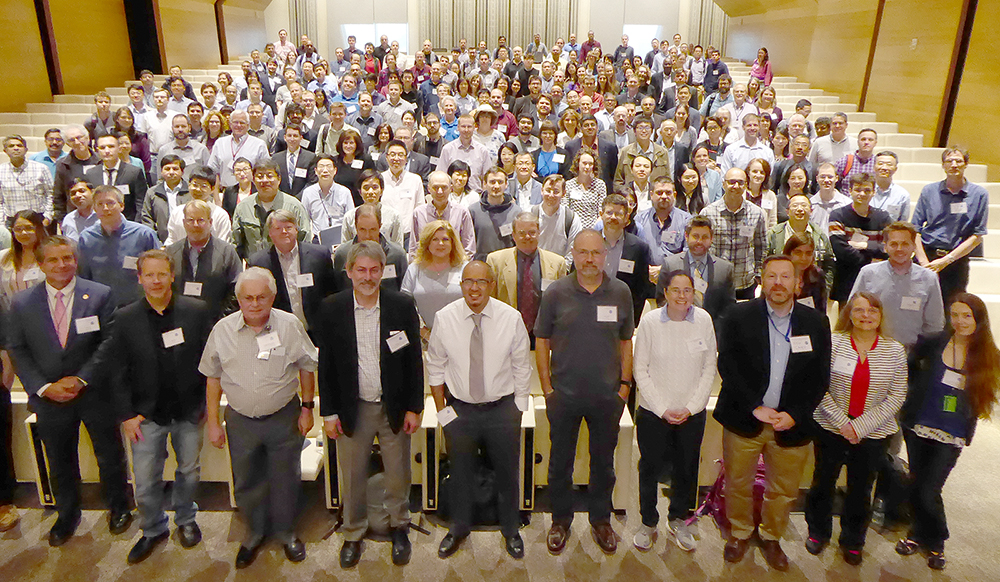
\includegraphics[width=0.45\linewidth]{figs/AIWkshp2019_grouppic_1000x582.jpg}
\end{figure}
\end{frame}

%----------------------------------------------------------------------------------------
%	PRESENTATION SLIDES
%----------------------------------------------------------------------------------------

\section{General Trends and Messages}

\begin{frame}
\frametitle{Satellite data used in assimilation current methods: (Christina Kumler)}
\begin{figure}
	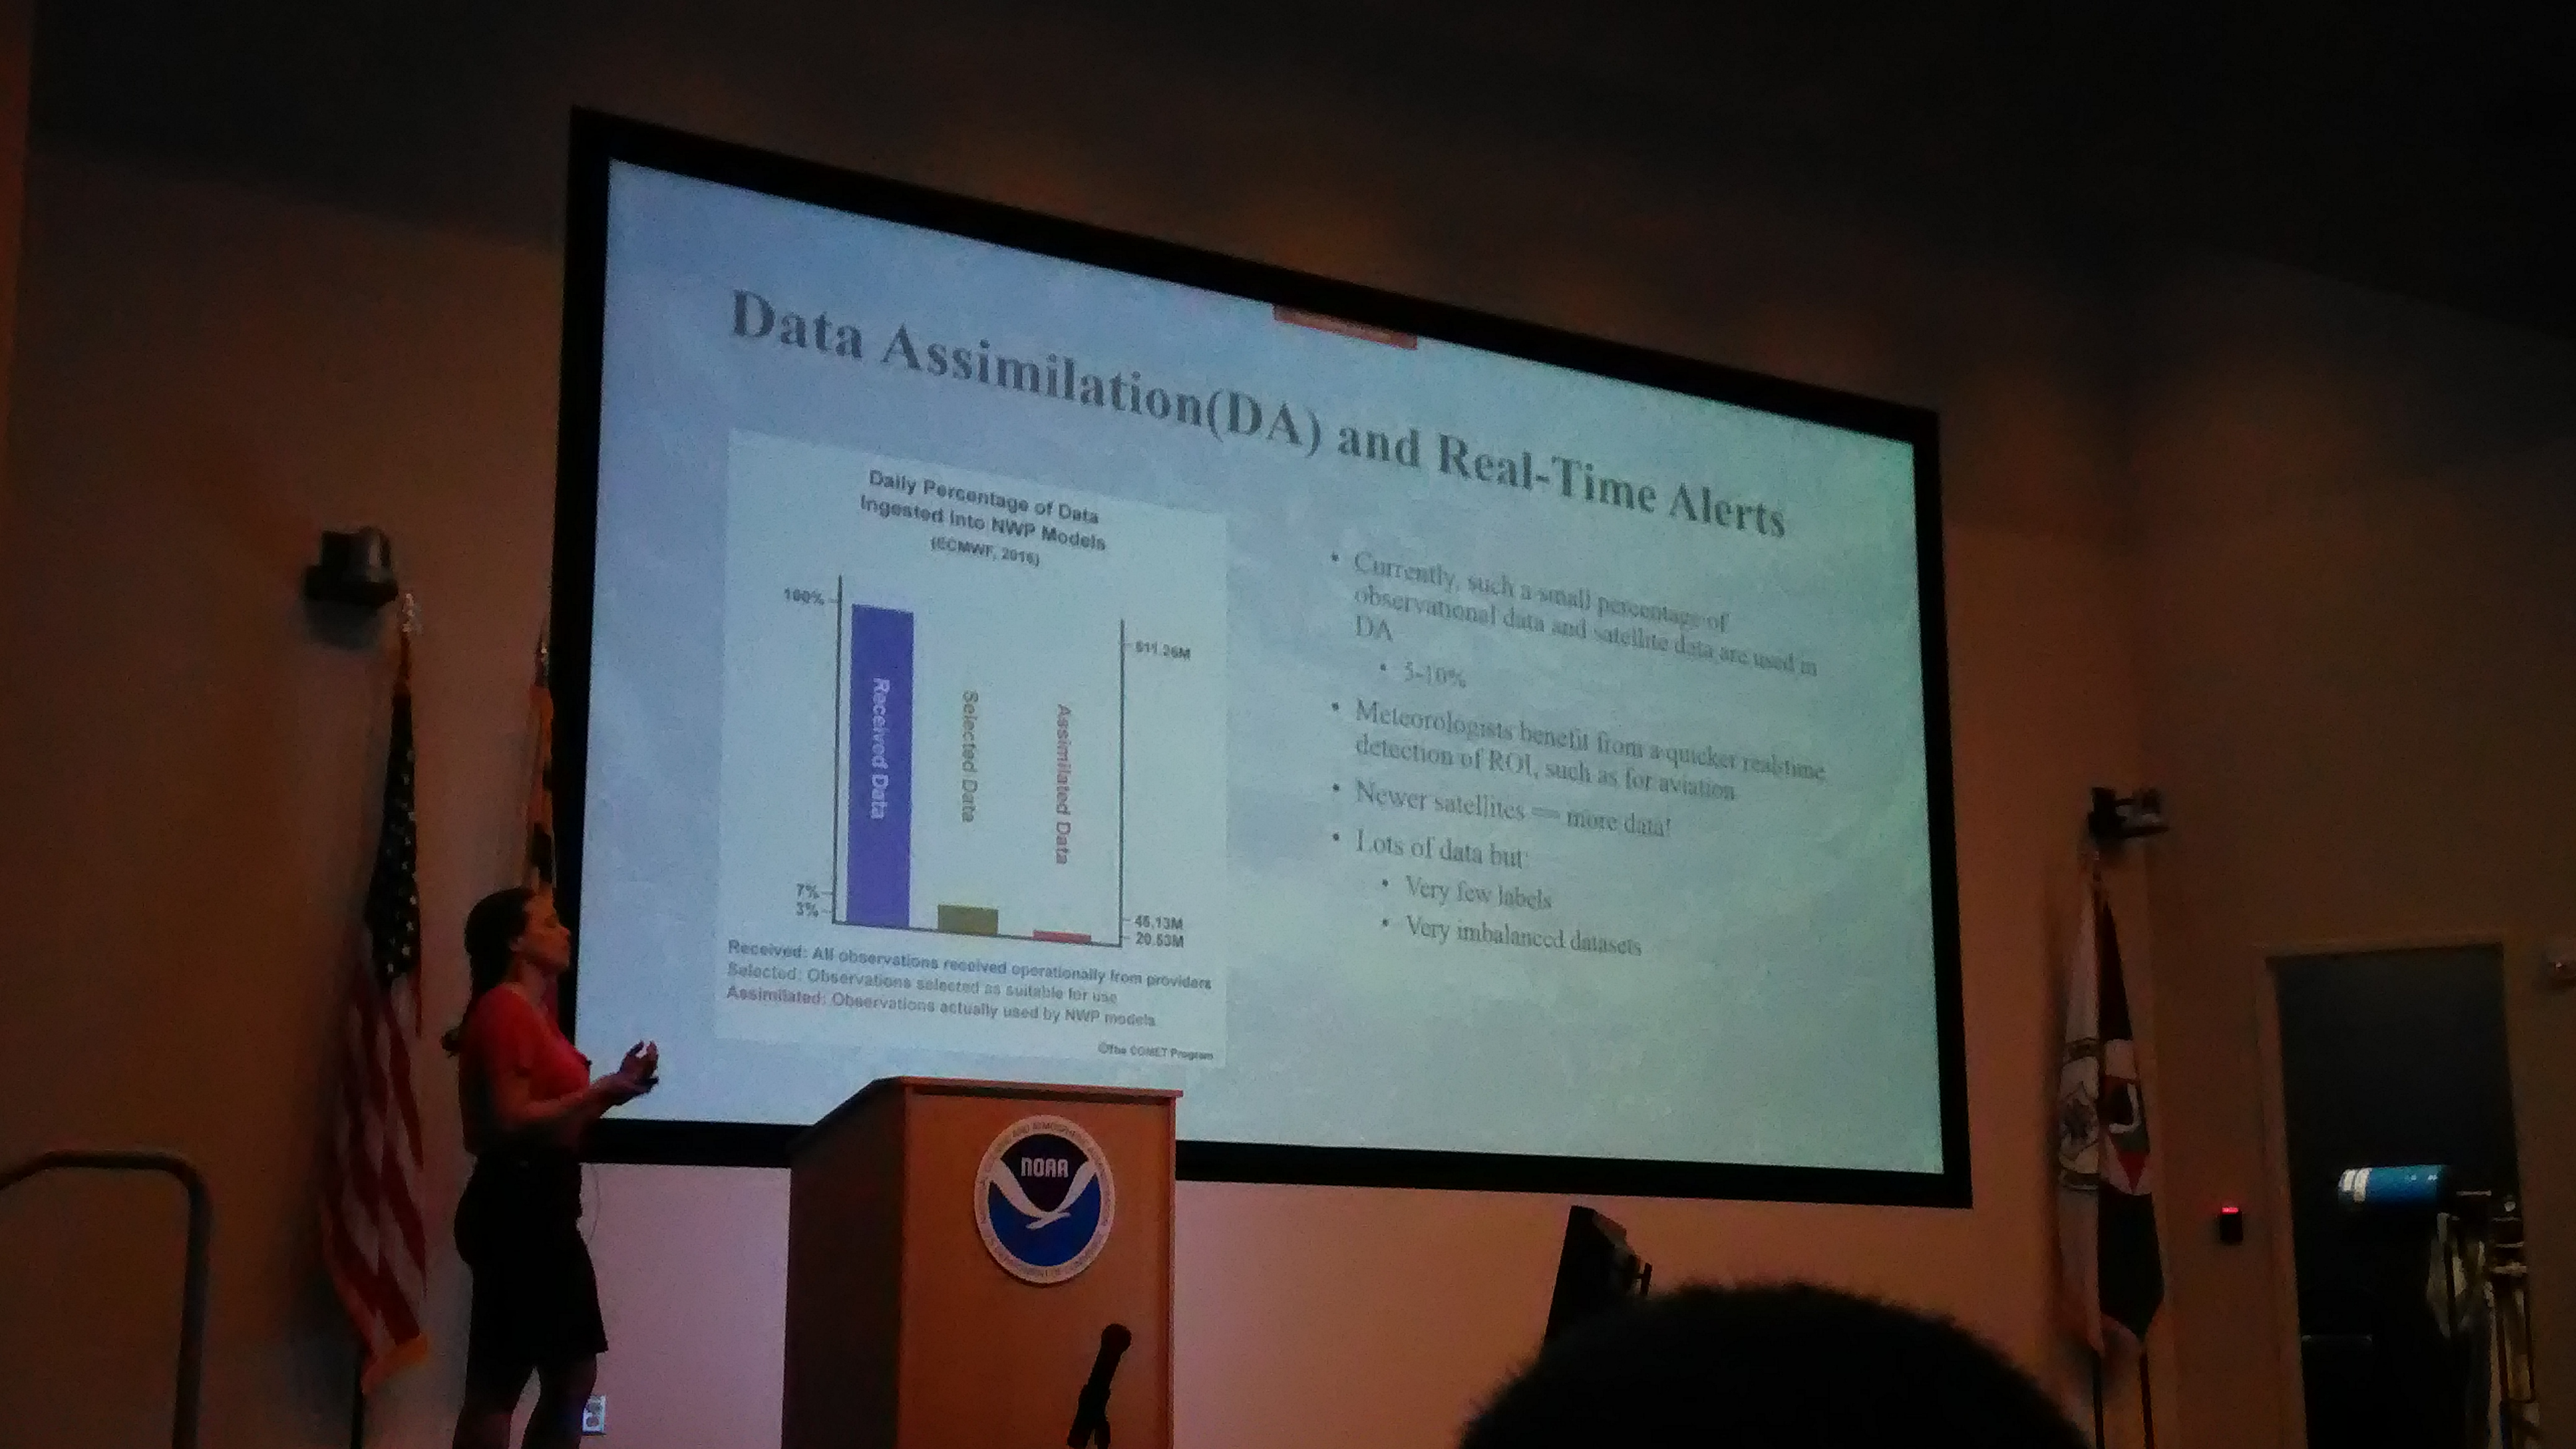
\includegraphics[width=\linewidth]{figs/P_20190424_091240.jpg}
\end{figure}
\end{frame}


\begin{frame}
\frametitle{Introduction talks (heads of NOAA, NWS,..)}

\begin{itemize}

\item Statements: 
	\begin{itemize}
		\item 100 Tb/day stored from satellite data
		\item ... only 5\% used
		\item too important runtimes of models (for now)
		\item everybody has a personal copy of the data...
	\end{itemize}
\item REAL need of AI:
	\begin{itemize}
		\item "drawning in an ocean of data"
		\item "we need help"
		\item "numerical weather prediction is not driving the market" (unlike medicine)
	\end{itemize}
\item How/where to use AI?
	\begin{itemize}
		\item uncertainty quantification (Florida, state of emergency launched 6 days before in 2018)
		\item fuse data from different satellites
		\item develop new applications
	\end{itemize}
\item New head of NOAA (Neil Jacobs)...
\end{itemize}
\end{frame}



\begin{frame}
\frametitle{Role/Potential of AI - Philip Tissot, AMS AI}
\begin{figure}
	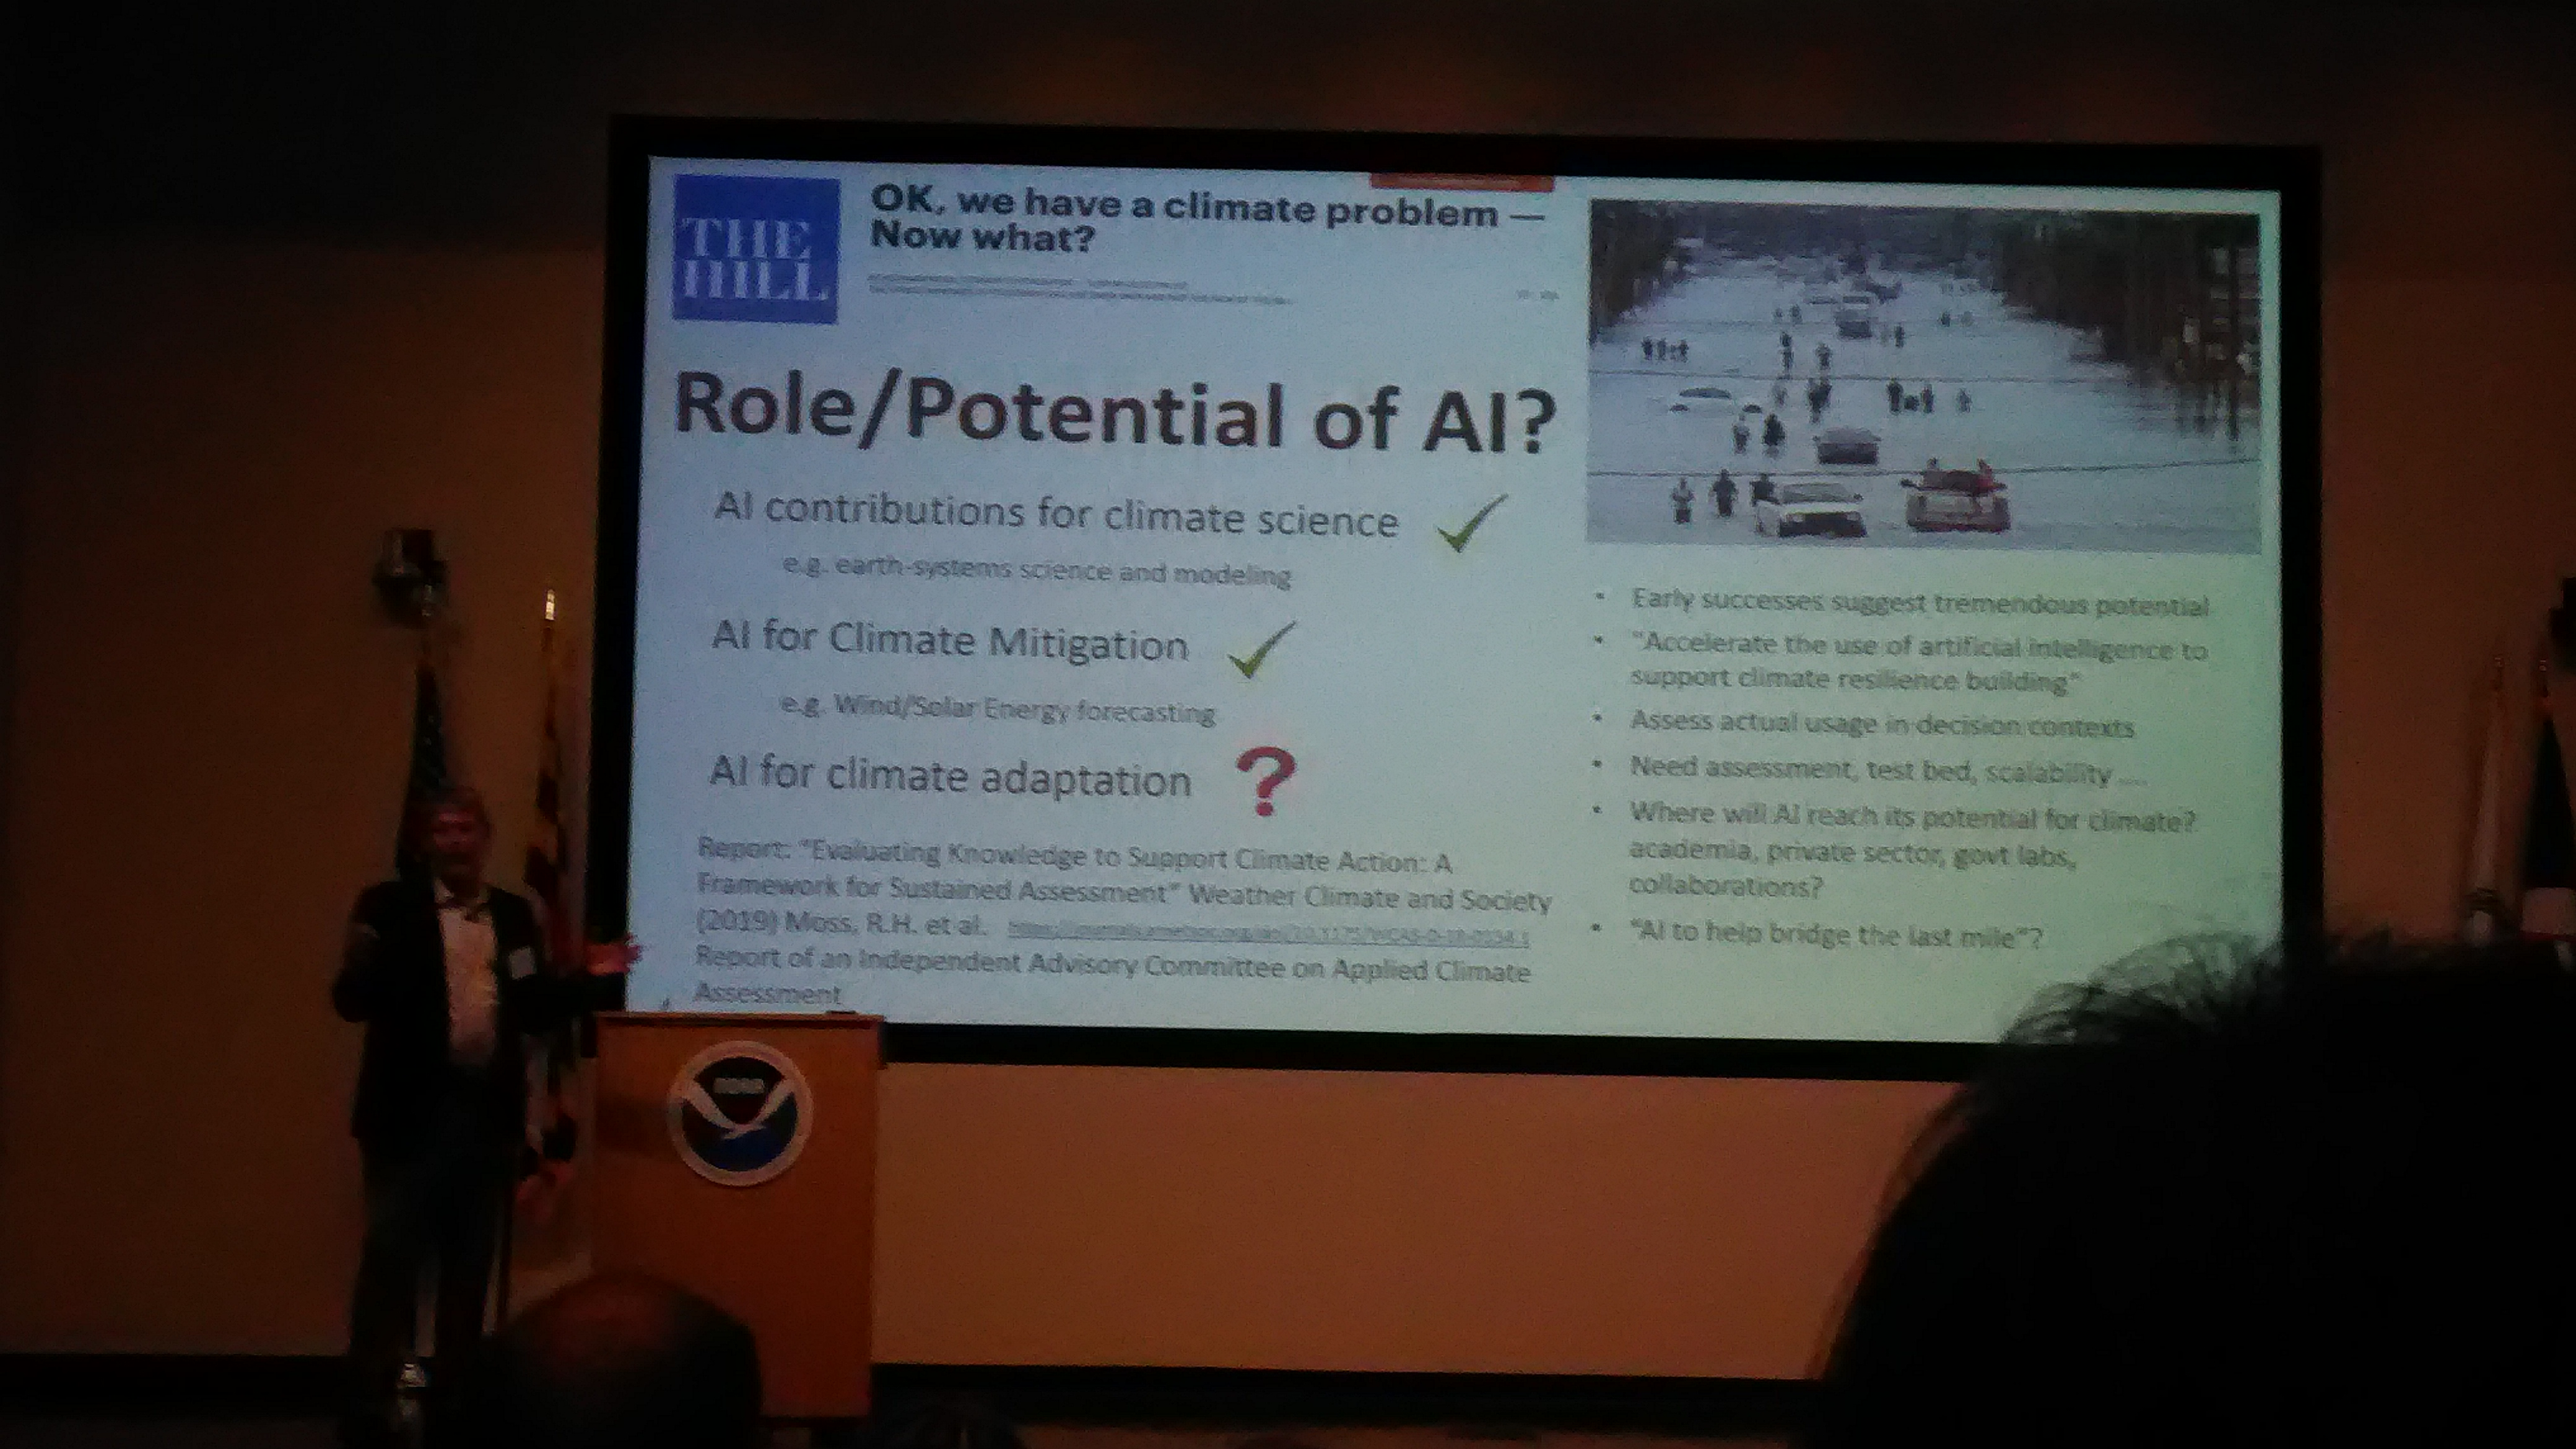
\includegraphics[width=\linewidth]{figs/P_20190423_105016.jpg}
\end{figure}
\end{frame}



\begin{frame}
\frametitle{Feelings about the Workshop}

\begin{itemize}
	\item Meteorologists are really willing to use ML
	\item They often don't know how to (correctly) do
	\item ... but would like to collaborate
	\item Companies are not really solving their problems
		\begin{itemize}
			\item ex. Microsoft presenting 'AI for Earth' and PAWS (protection assistant for wildlife security)
			\item ex. Google, just wanted to sell their 'TPU'
			\item ex. Nvidia (David Hall) : 'we want to make cool videos' 
		\end{itemize}
\end{itemize}
\end{frame}

\begin{frame}
\frametitle{Sid Boukabara, NOAA \textit{(Overview of NOAA AI activities in satellite obs. and NWP)}}
\begin{figure}
	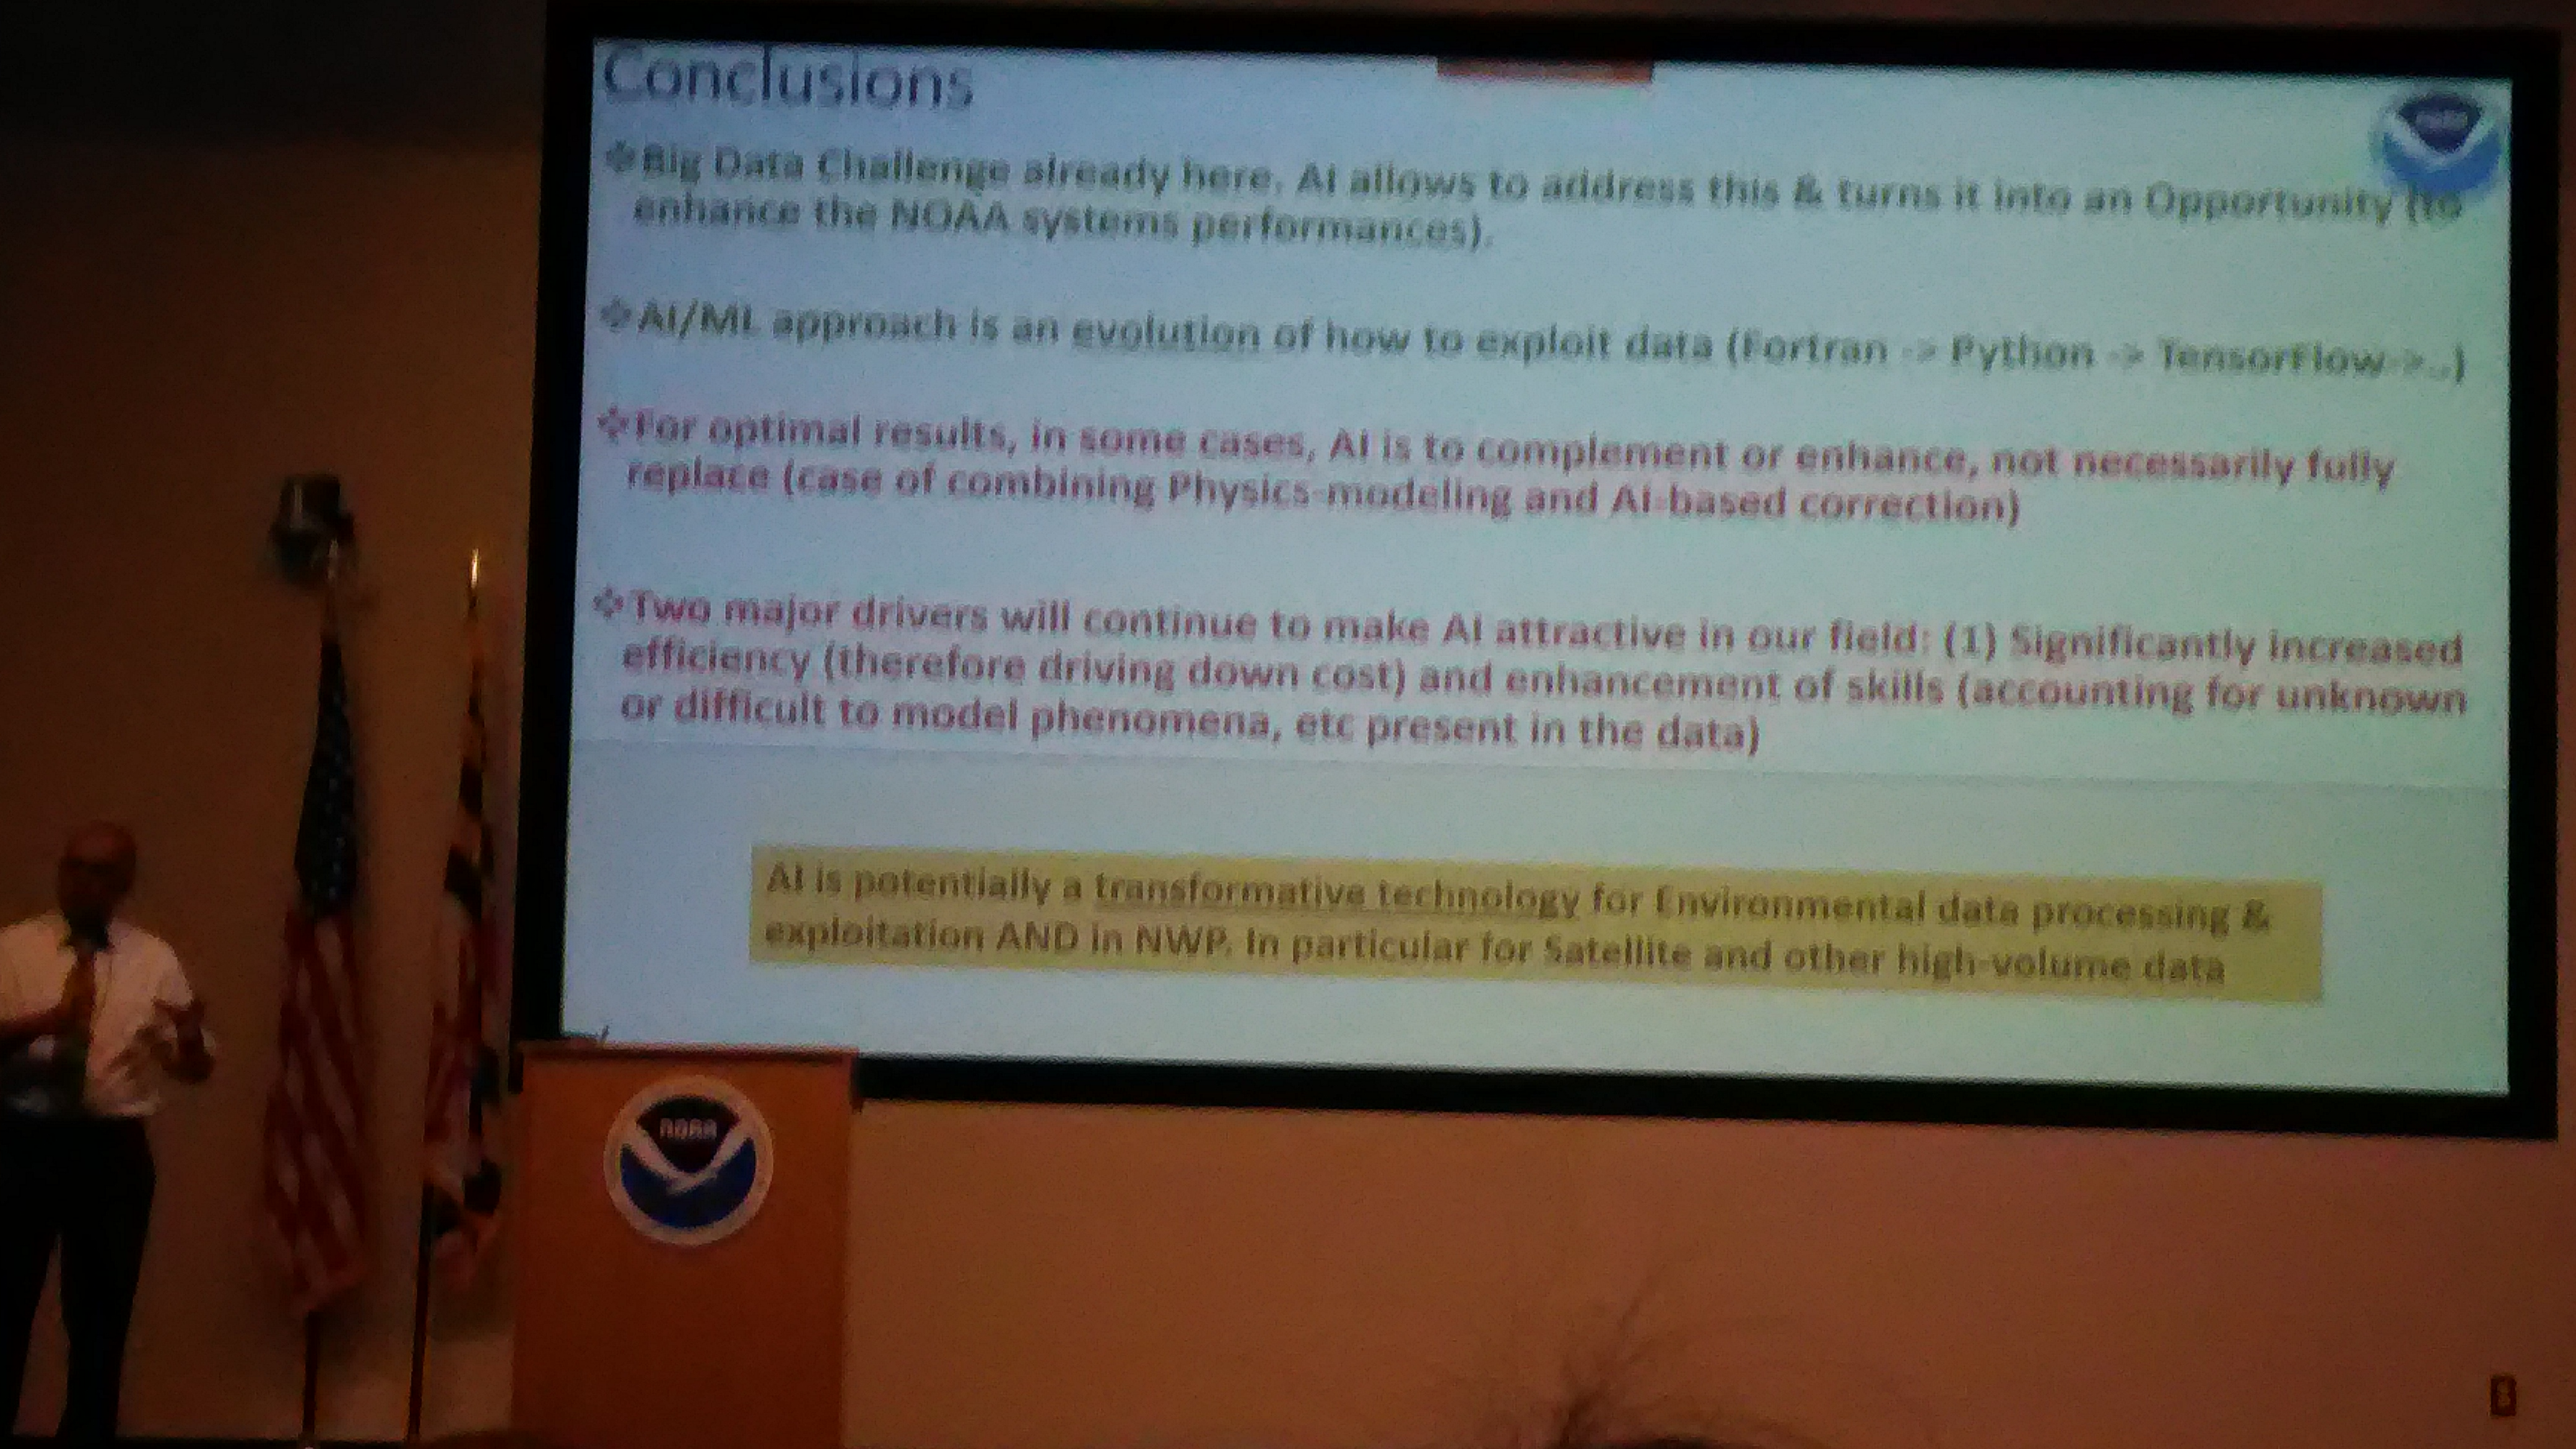
\includegraphics[width=\linewidth]{figs/P_20190423_111607.jpg}
\end{figure}
\end{frame}



\begin{frame}
\frametitle{Interesting Materials or Links}

\begin{itemize}
	\item Conferences: 
	\begin{itemize}
	\item AMS AI Conference (Boston Jan 11-16 2020)
	\item SCAN organization (Science for Climate Action Network)
	\item Alpha-institute (to build) - Amy McGovern (AI and climate/weather collaborations)
\end{itemize}		
	\item Datasets: 
	\begin{itemize}
	\item EnviroNet / ClimateNet (tropical cyclones/atm rivers)
	\item Google Earth Engine Data Catalog (https://developers.google.com/earth-engine/datasets/)
	\item NASA dataset : SMAP Data (Soil Moisture Active Passive Data)
	\end{itemize}		
	
	\item Tools: 
	\begin{itemize}
	\item End-to-end python pipeline (GPU) RAPIDS (Nvidia)
	\item open-source earth-system model of energy/weather issues https://e3sm.org/
	\item UMD-NASA work on partial convolution: MENSA data processing environment available soon
	\end{itemize}
	
\end{itemize}
\end{frame}

\begin{frame}
\frametitle{Amy McGovern, University of Oklahoma \textit{(Alpha institute)}}
\begin{figure}
	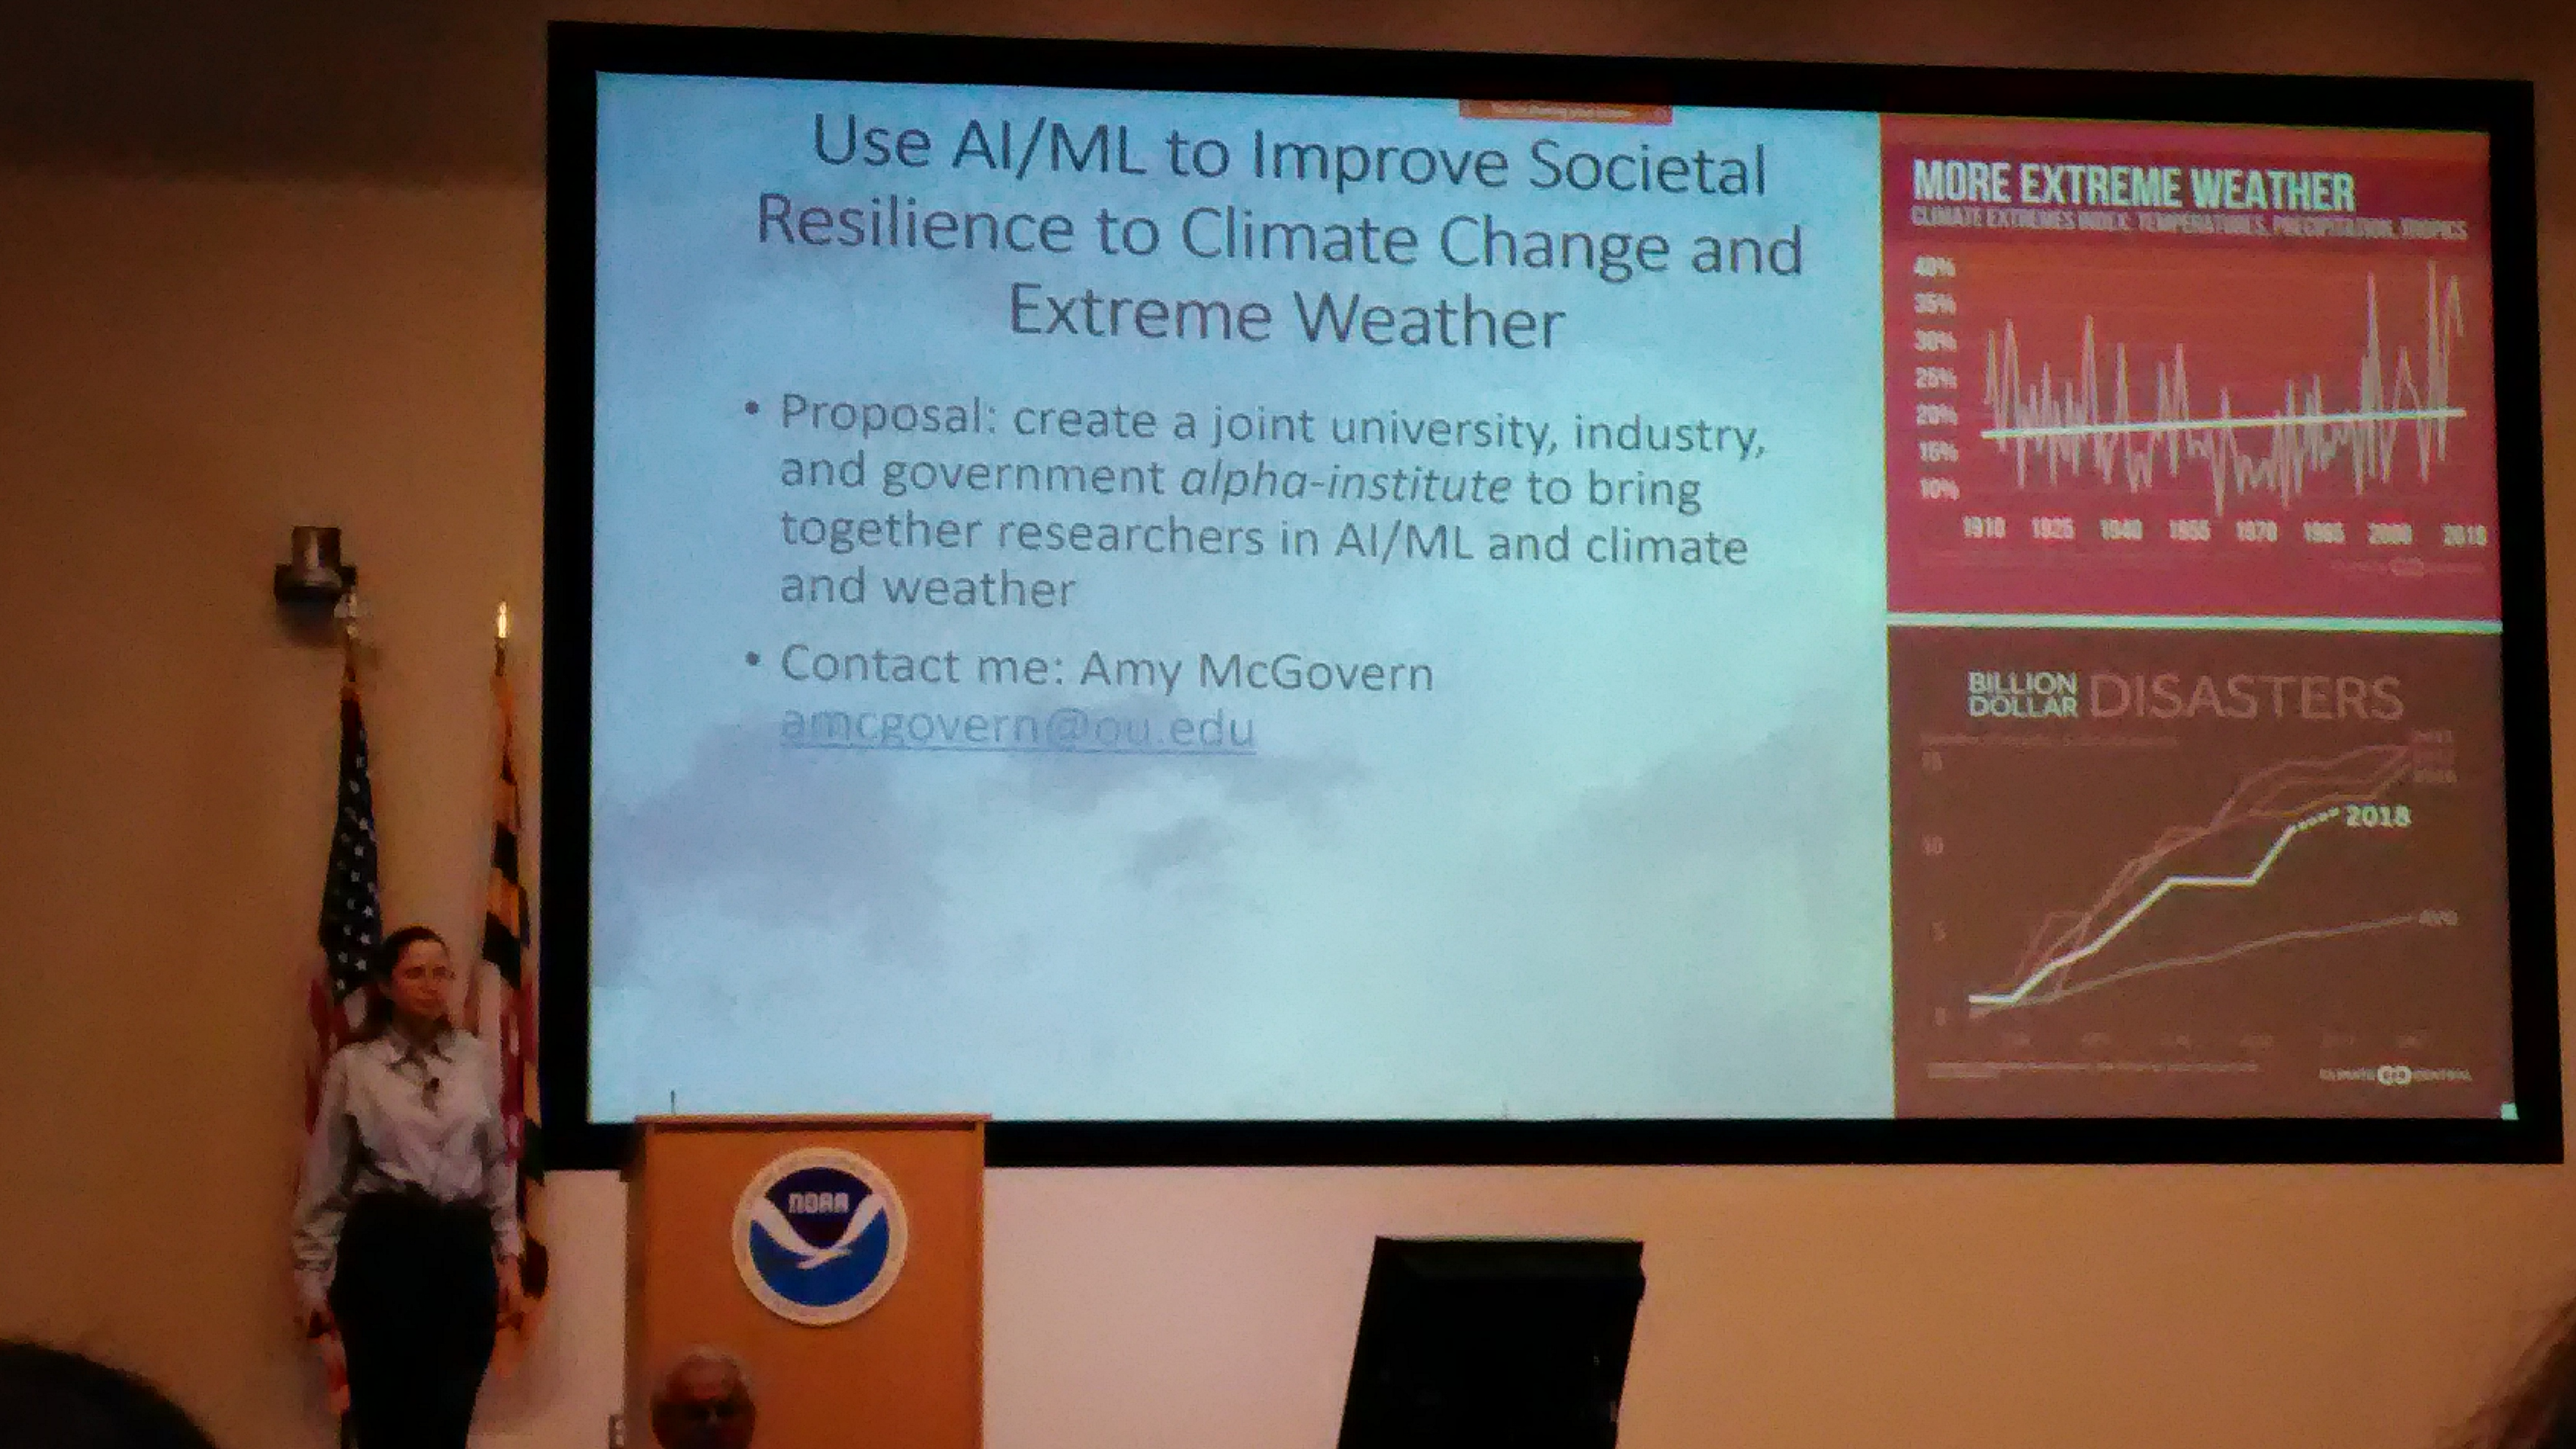
\includegraphics[width=\linewidth]{figs/P_20190425_105024.jpg}
\end{figure}
\end{frame}

\begin{frame}
\frametitle{SCAN organization (Science for Climate Action Network) - Philip Tissot, AMS AI}
\begin{figure}
	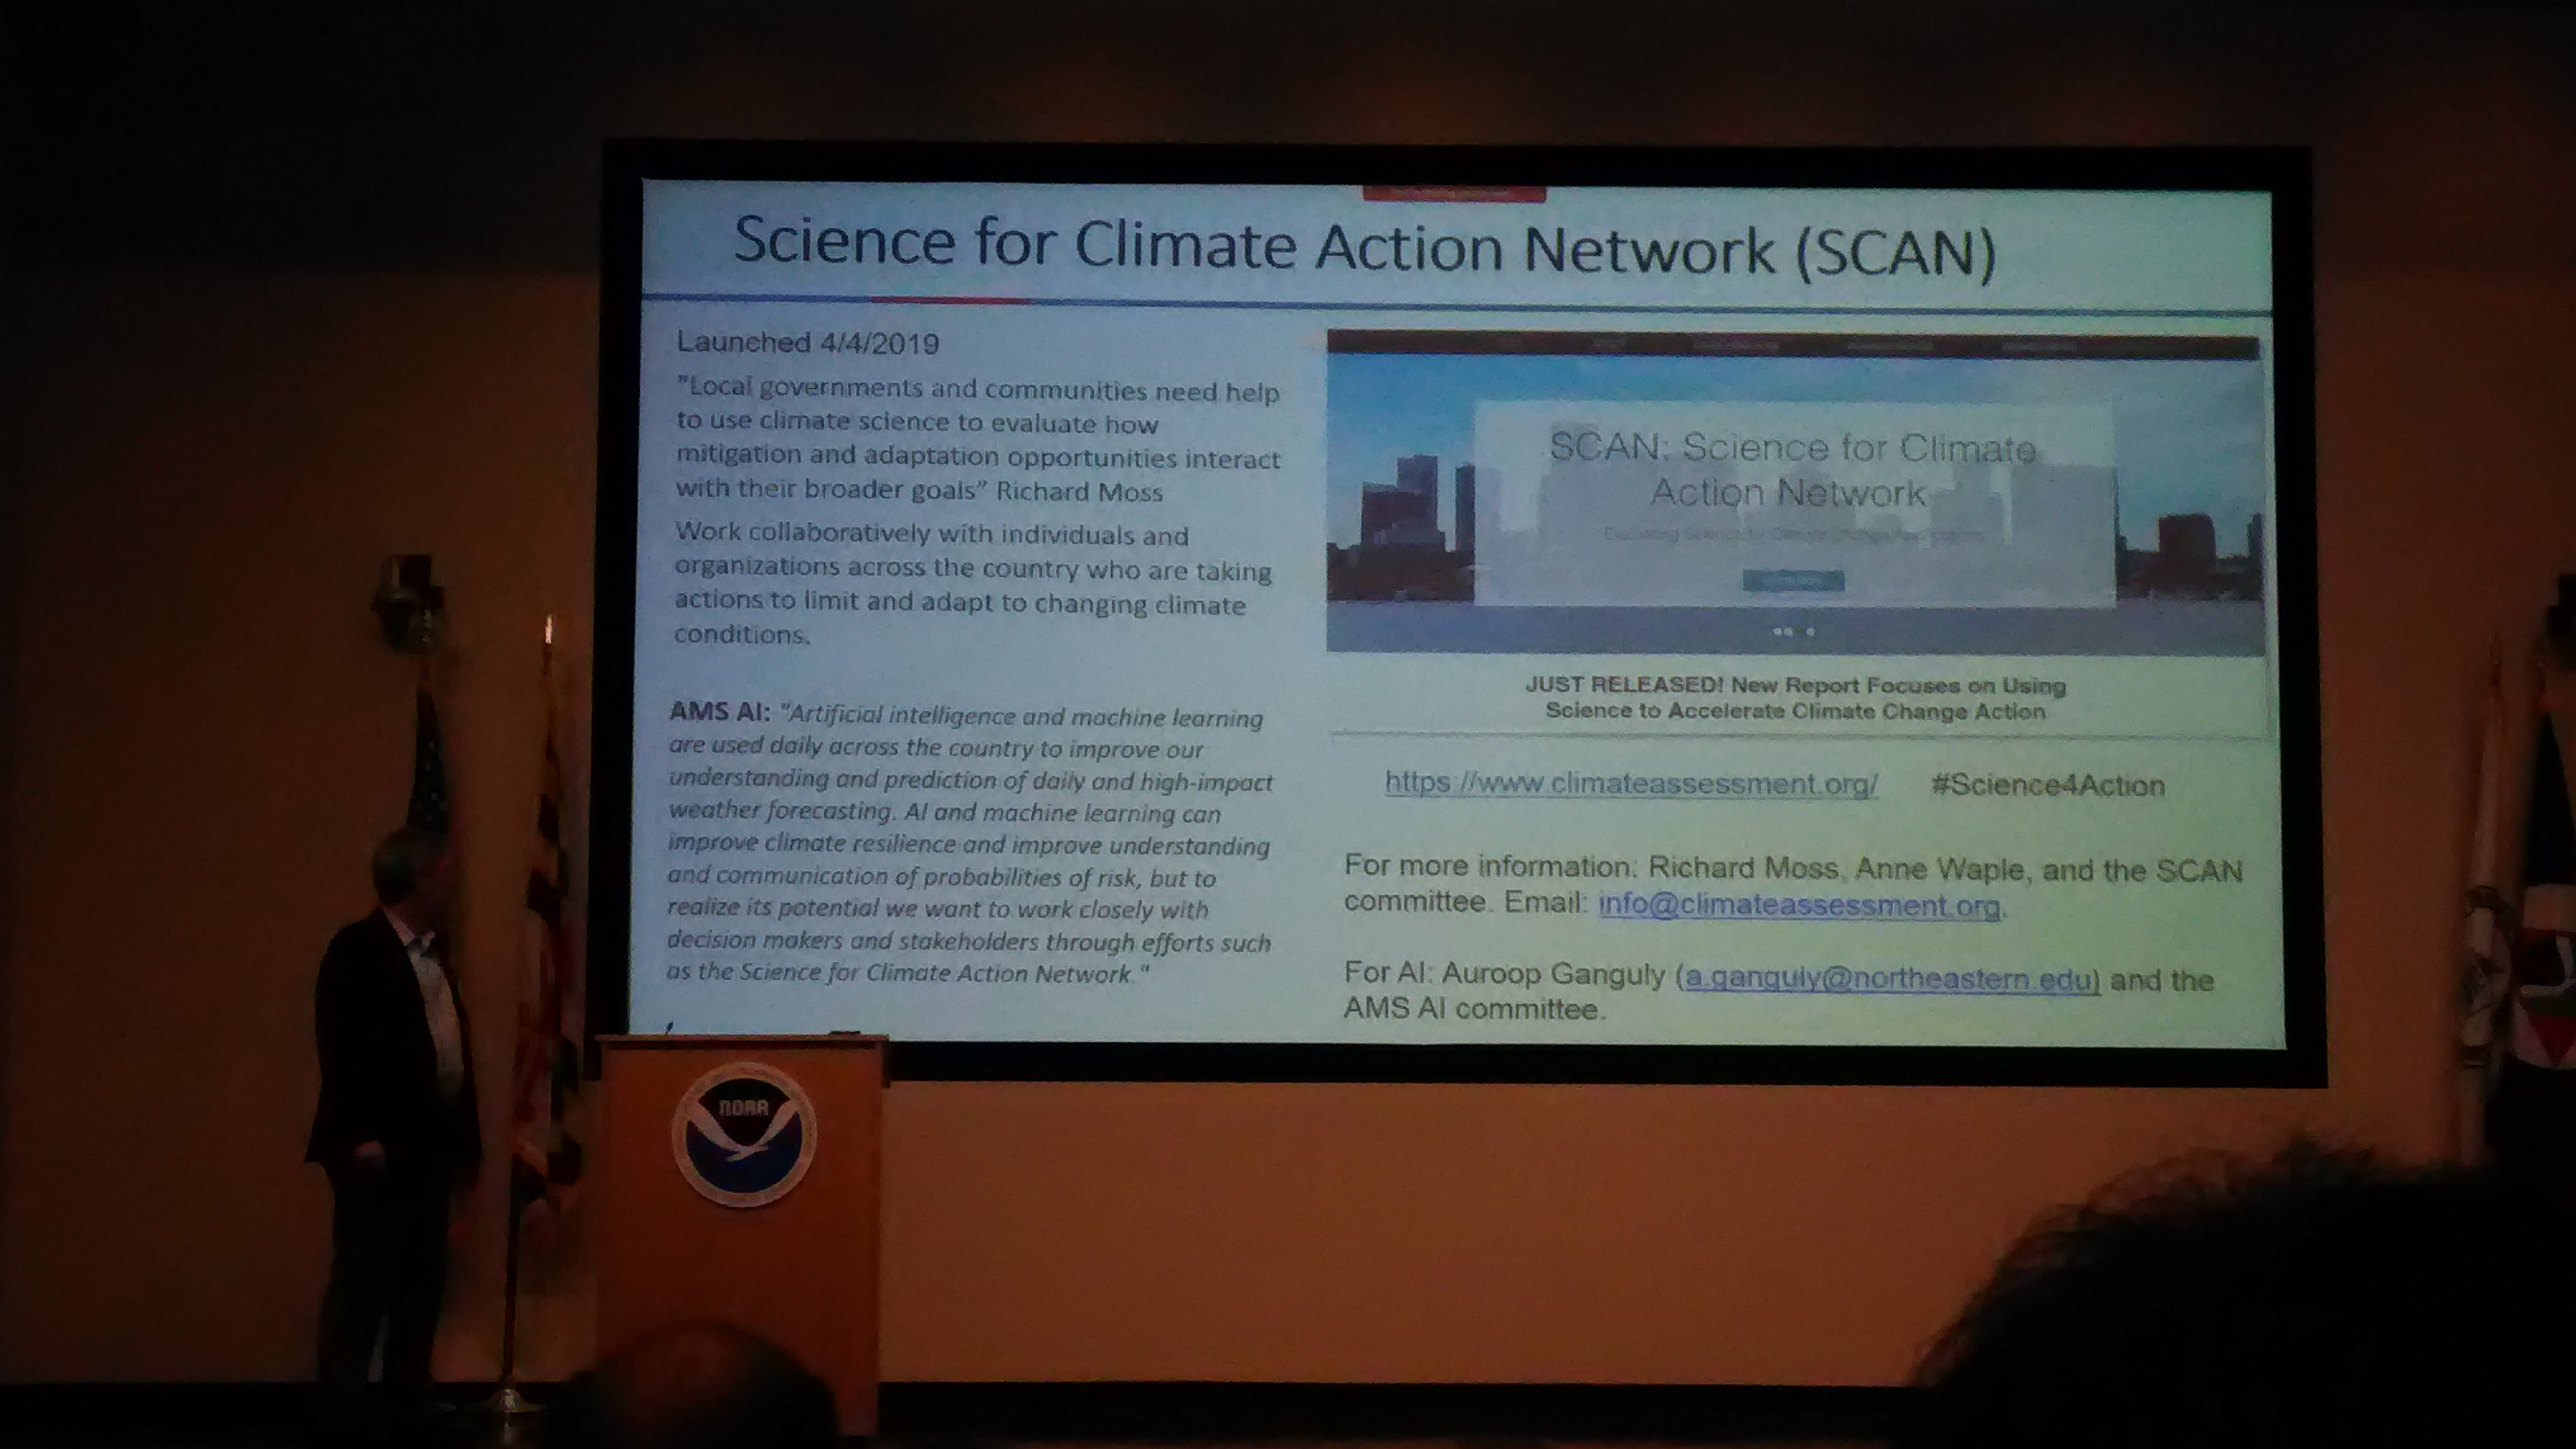
\includegraphics[width=\linewidth]{figs/P_20190423_105212.jpg}
\end{figure}
\end{frame}

\section{Interesting Talks/Posters..}

\begin{frame}
\frametitle{Outline} % Table of contents slide, comment this block out to remove it
\tableofcontents[currentsection] % Throughout your presentation, if you choose to use \section{} and \subsection{} commands, these will automatically be printed on this slide as an overview of your presentation
\end{frame}
%
\subsection{ML methods}
\begin{frame}
\frametitle{Sarat Sreepathi, Oak Ridge National Lab
 \textit{(EarthInsights: parallel clustering of large earth science datasets on summit supercomputer)}}
 \begin{itemize}
\item clustering climate regimes (?), fire intensity/incidence, vegetation
\item assess regional impacts of climate change
\end{itemize}
\begin{figure}
	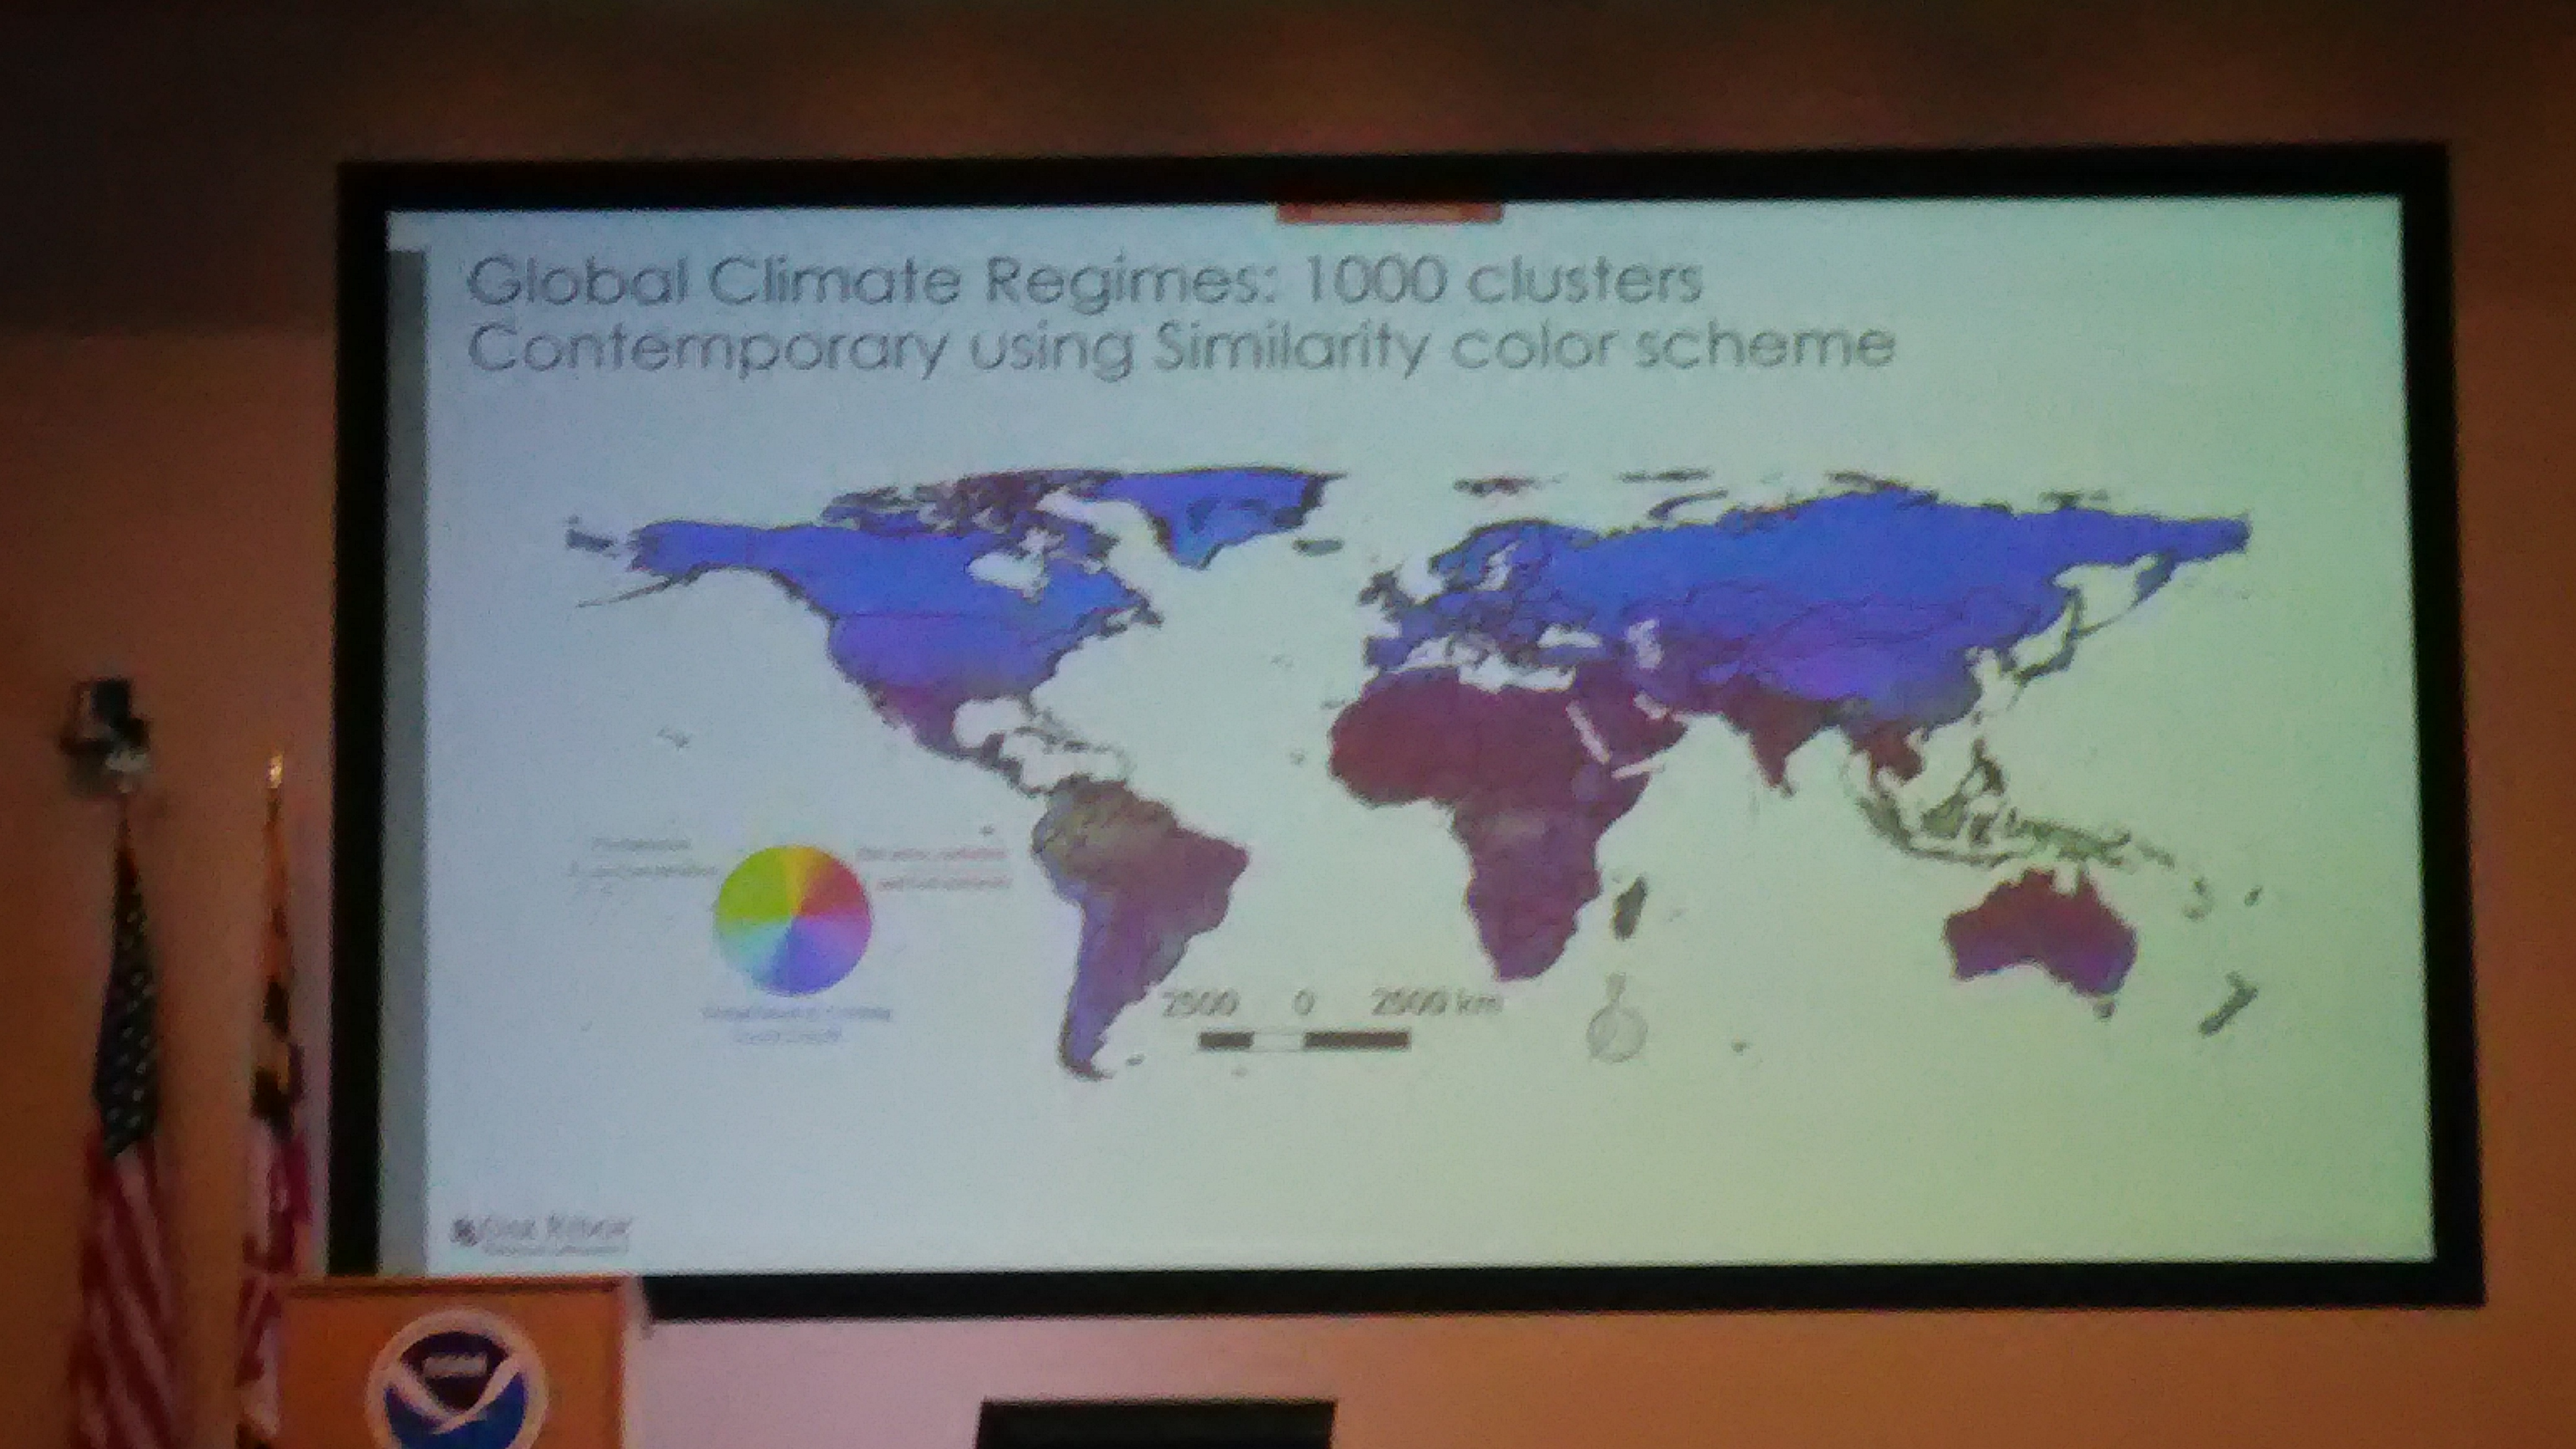
\includegraphics[width=.8\linewidth]{figs/P_20190424_104512.jpg}
\end{figure}
\end{frame}

\begin{frame}
\frametitle{Thomas Vandal, NASA \textit{(Intermediate frame interpolation to improve temporal coverage of GOES-16)}}
Frame interpolation using optical flow
\begin{figure}
	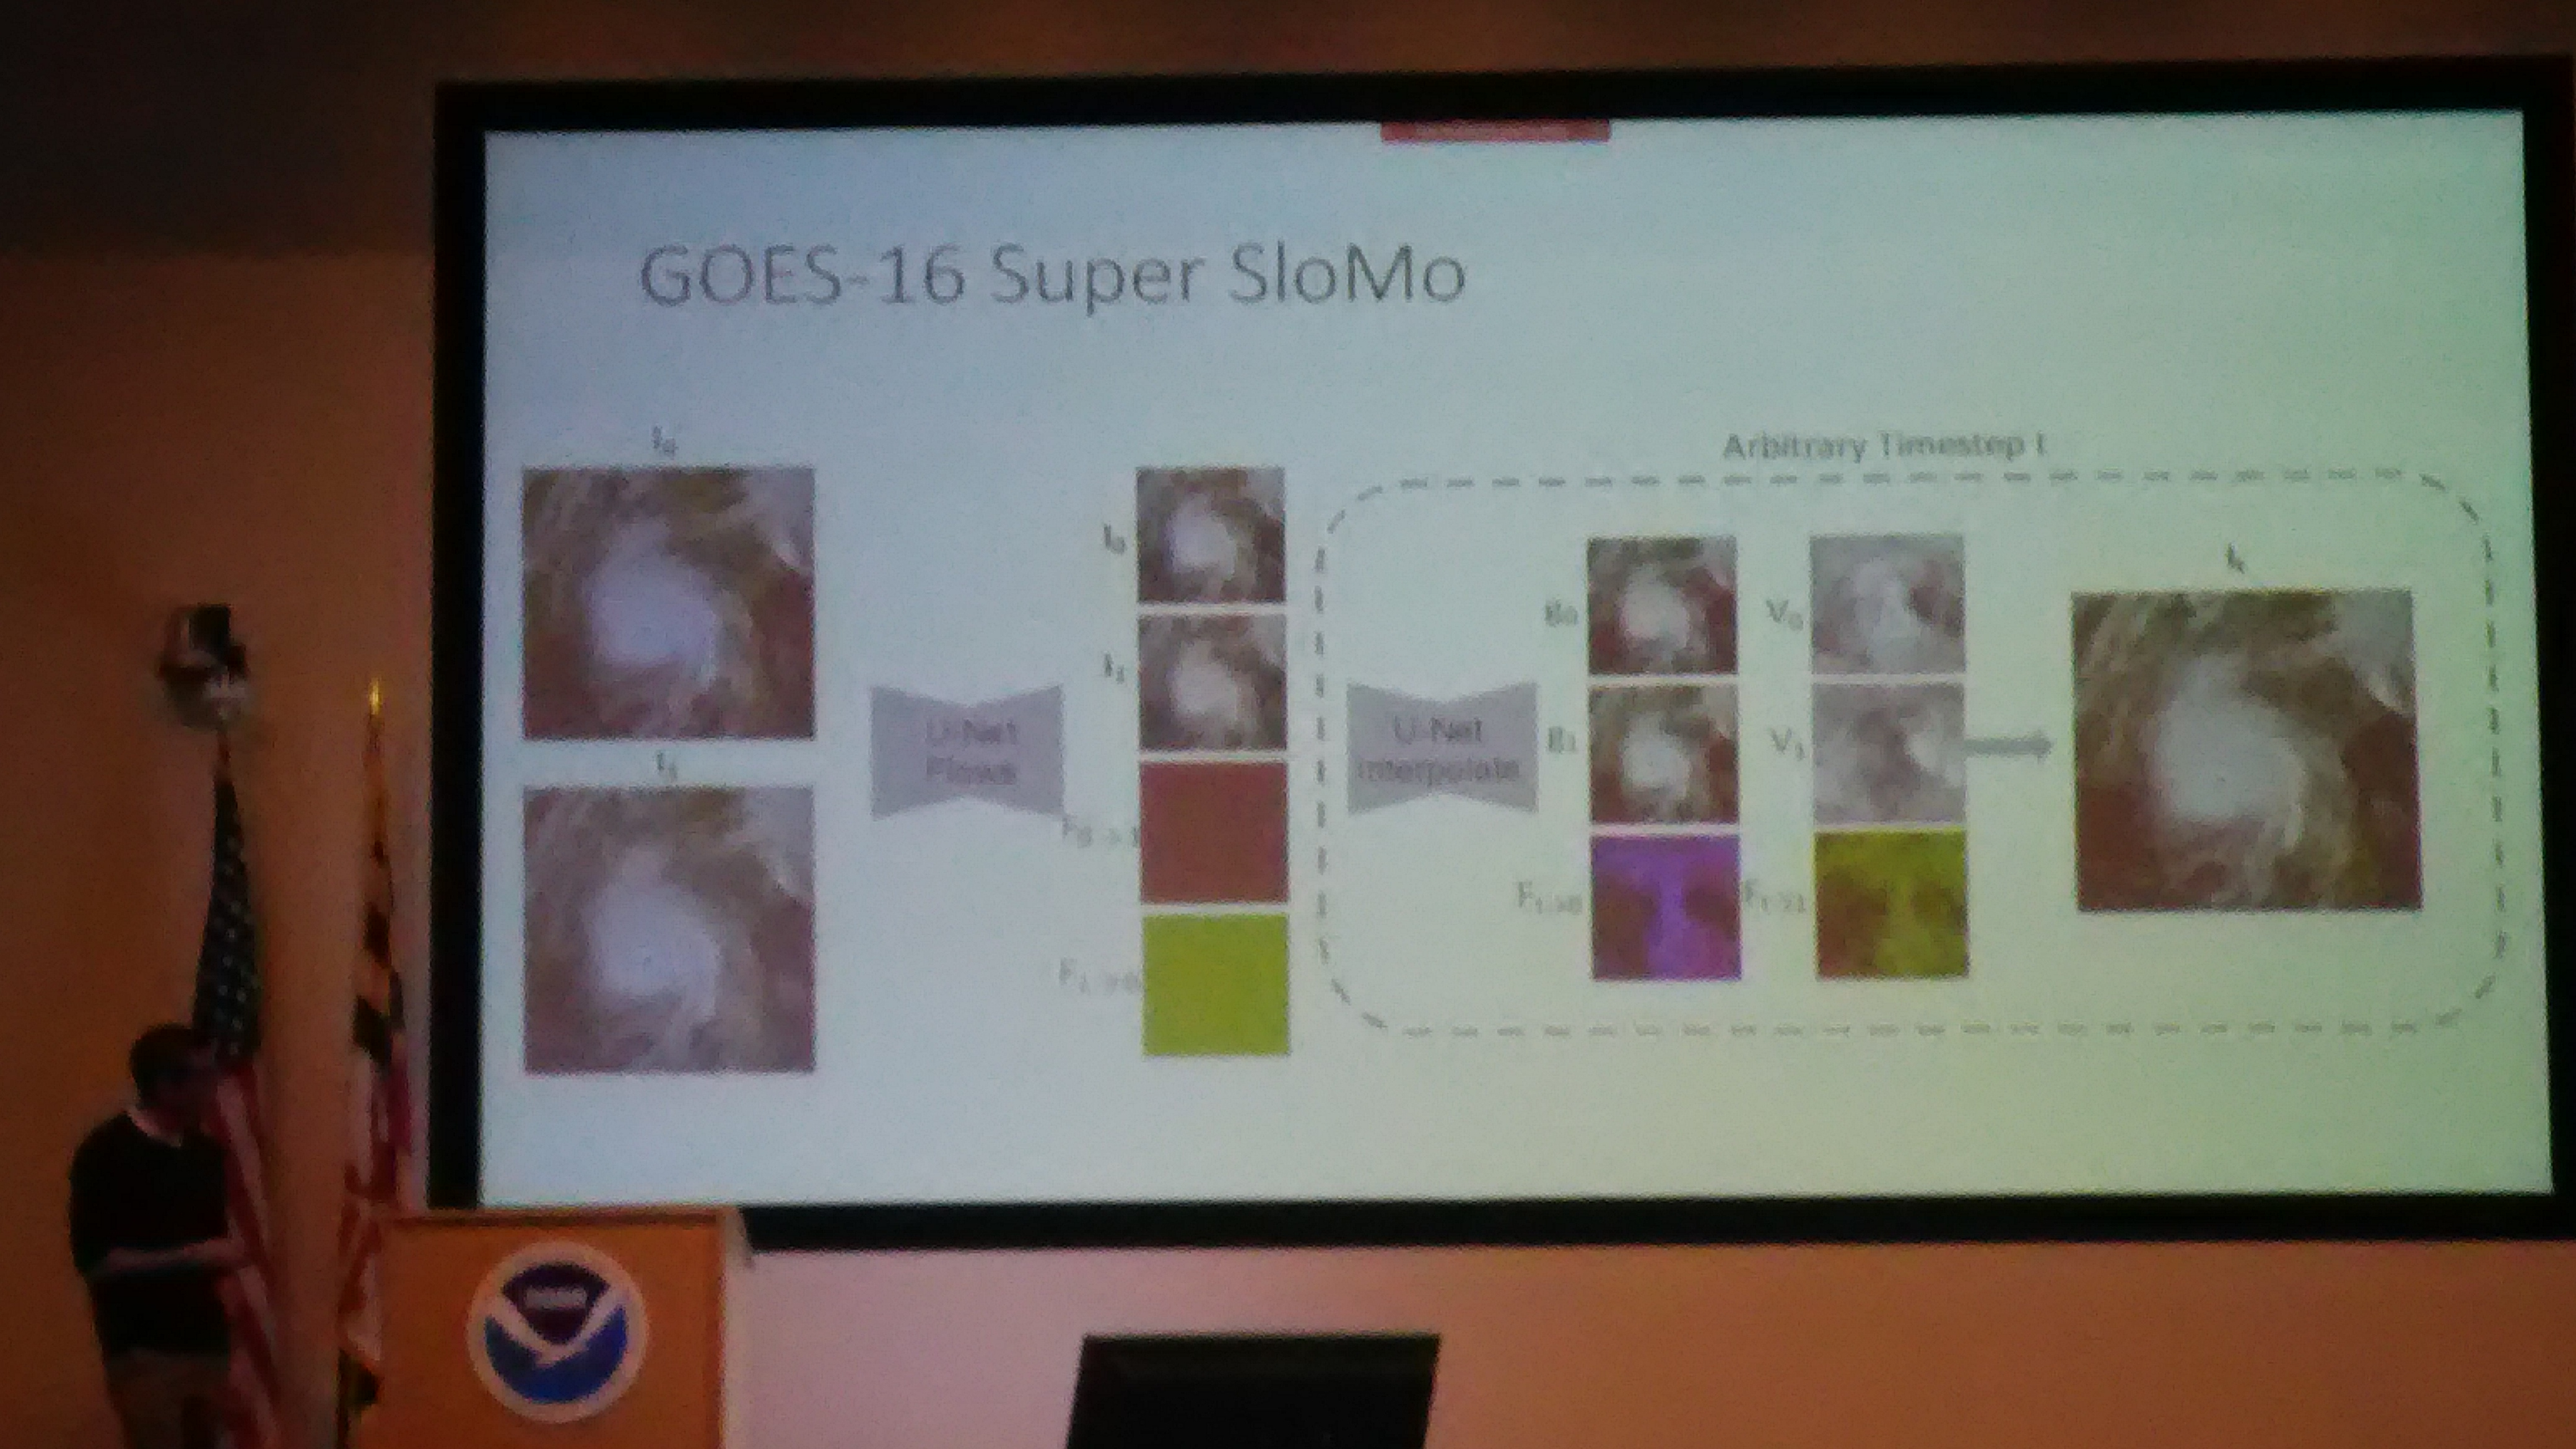
\includegraphics[width=.9\linewidth]{figs/P_20190424_111508.jpg}
\end{figure}
\end{frame}

\begin{frame}
\frametitle{Thomas Vandal, NASA \textit{(Intermediate frame interpolation to improve temporal coverage of GOES-16)}}
"Dropout as a Bayesian Approximation:
Representing Model Uncertainty in Deep Learning", Yarin Gal, Zoubin Ghahramani, University of Cambridge. 2016

\begin{figure}
	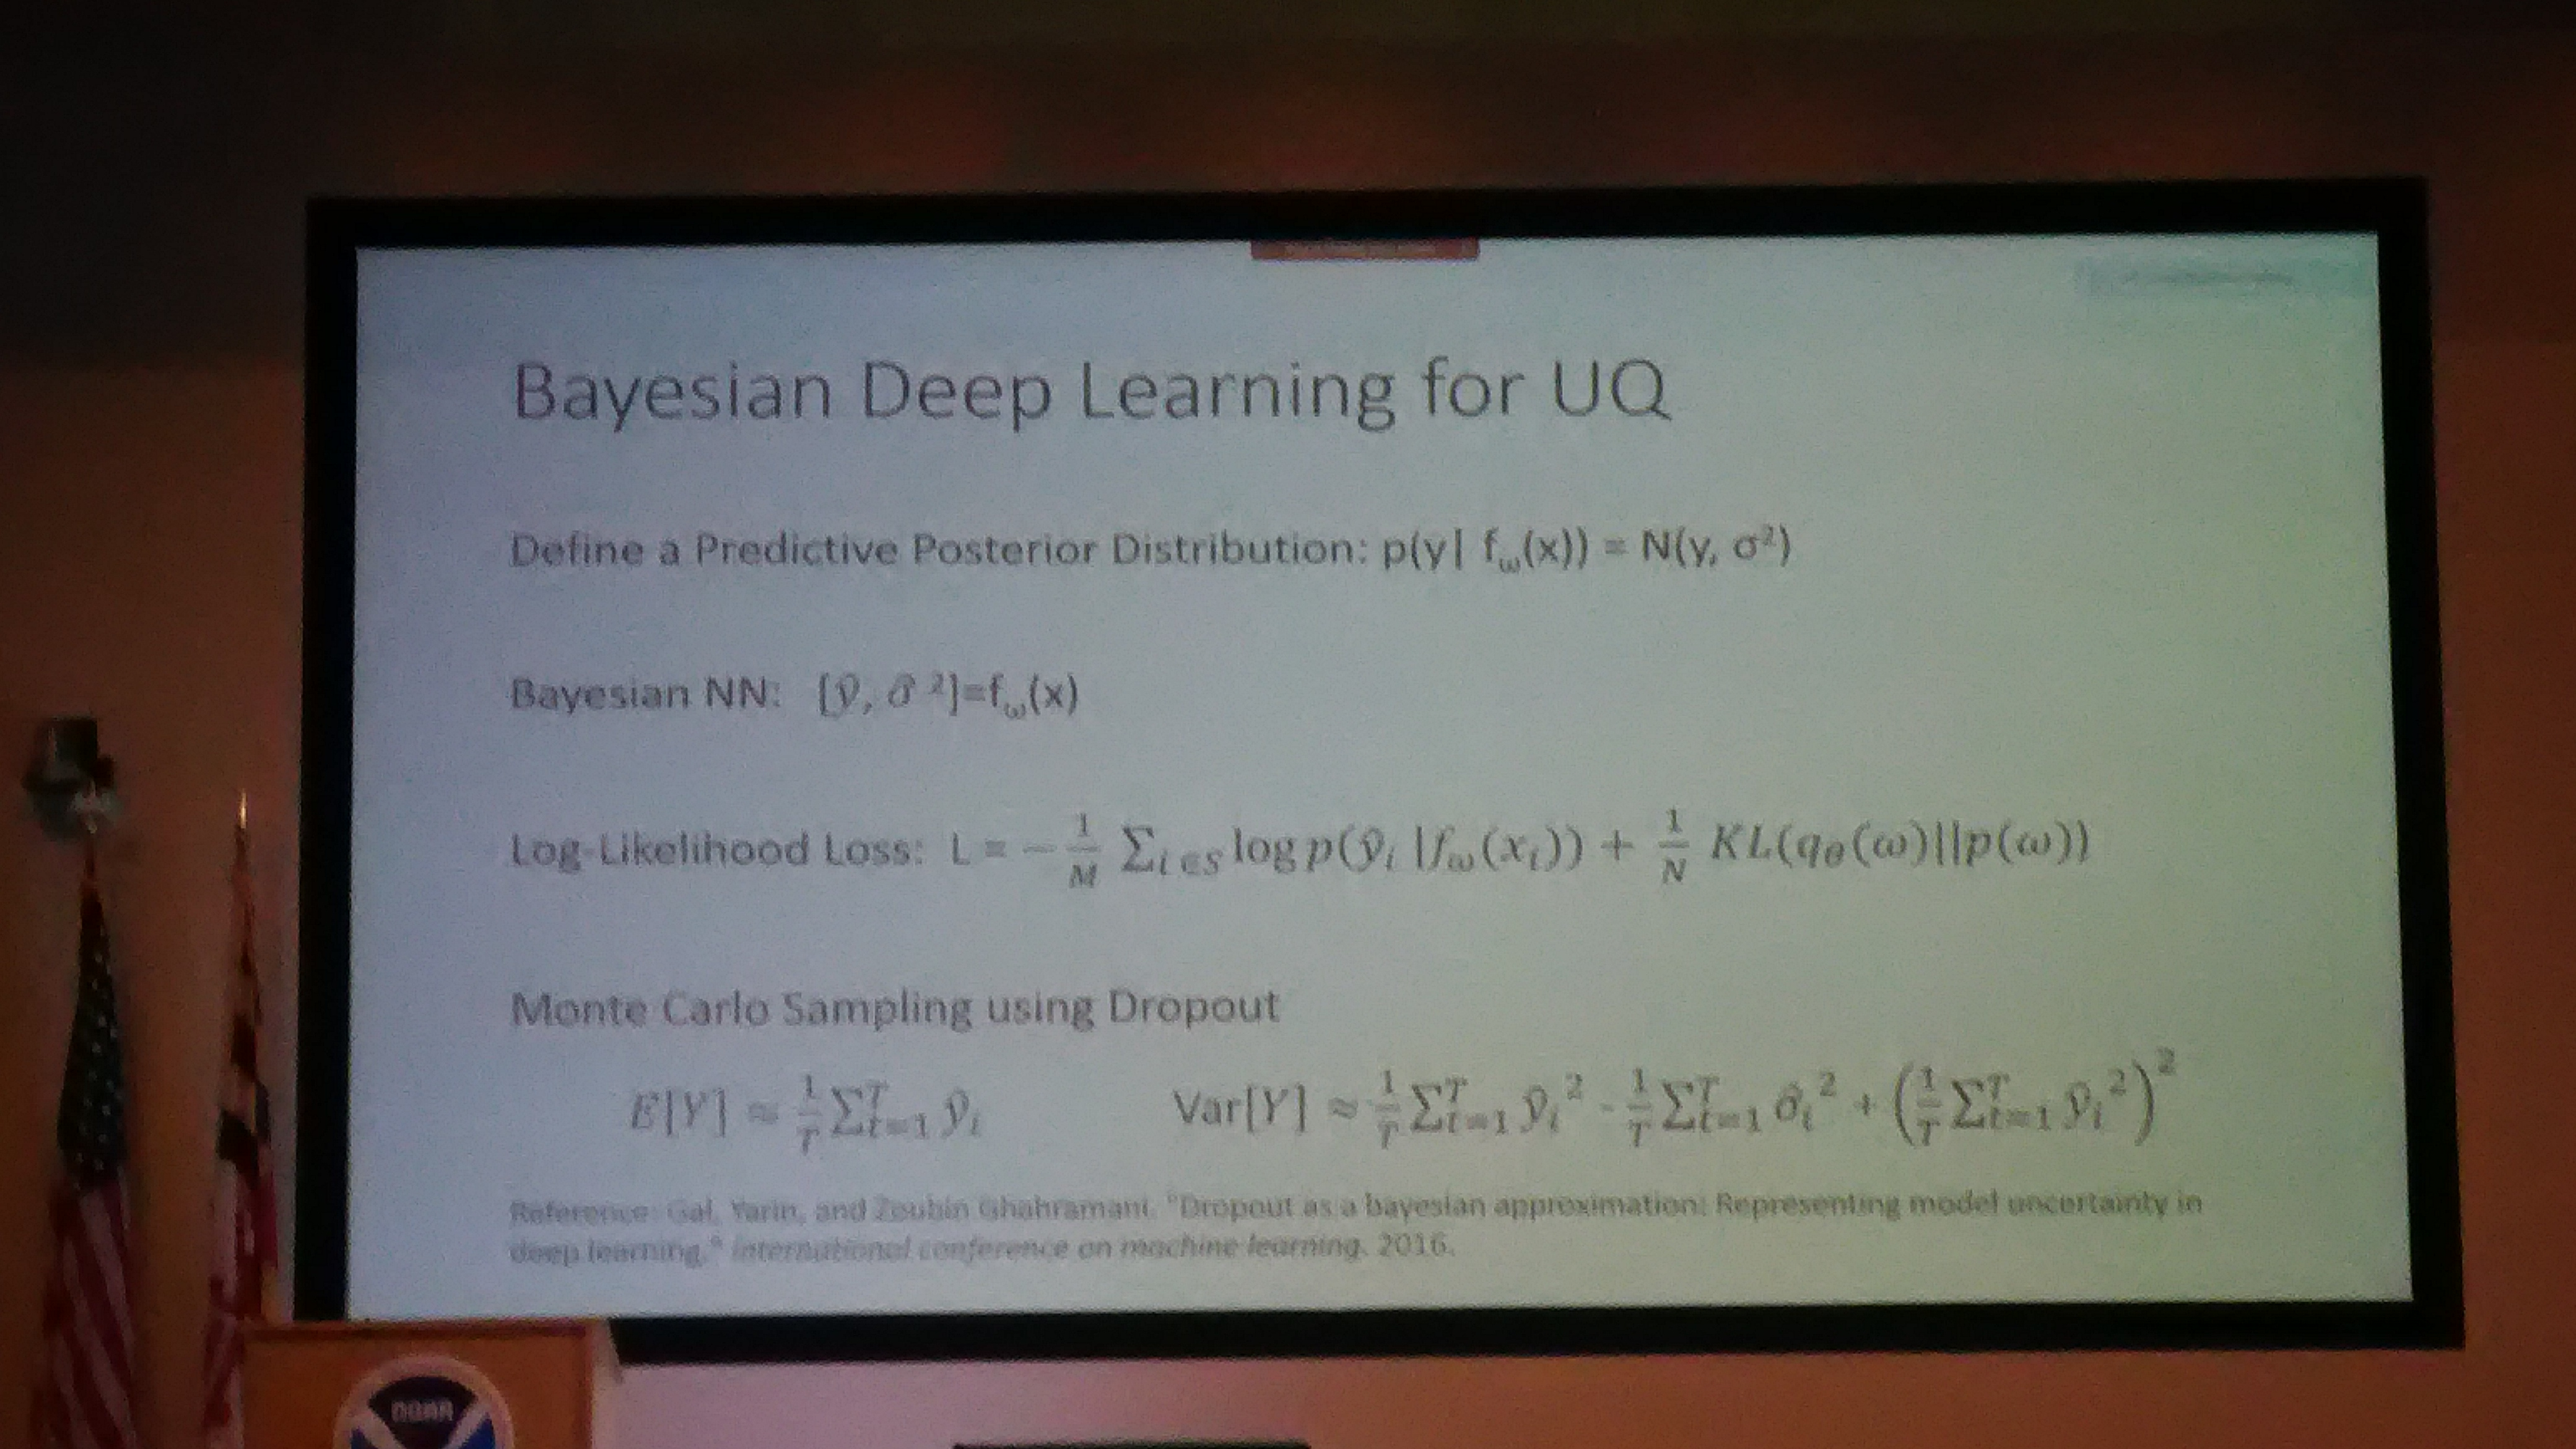
\includegraphics[width=.9\linewidth]{figs/P_20190424_112041.jpg}
\end{figure}
\end{frame}


\subsection{AI and physics}

\begin{frame}
\frametitle{Outline} % Table of contents slide, comment this block out to remove it
\tableofcontents[currentsection] % Throughout your presentation, if you choose to use \section{} and \subsection{} commands, these will automatically be printed on this slide as an overview of your presentation
\end{frame}

\begin{frame}
\frametitle{Chaopeng Shen, Pennsylvania State U.}
\begin{figure}
	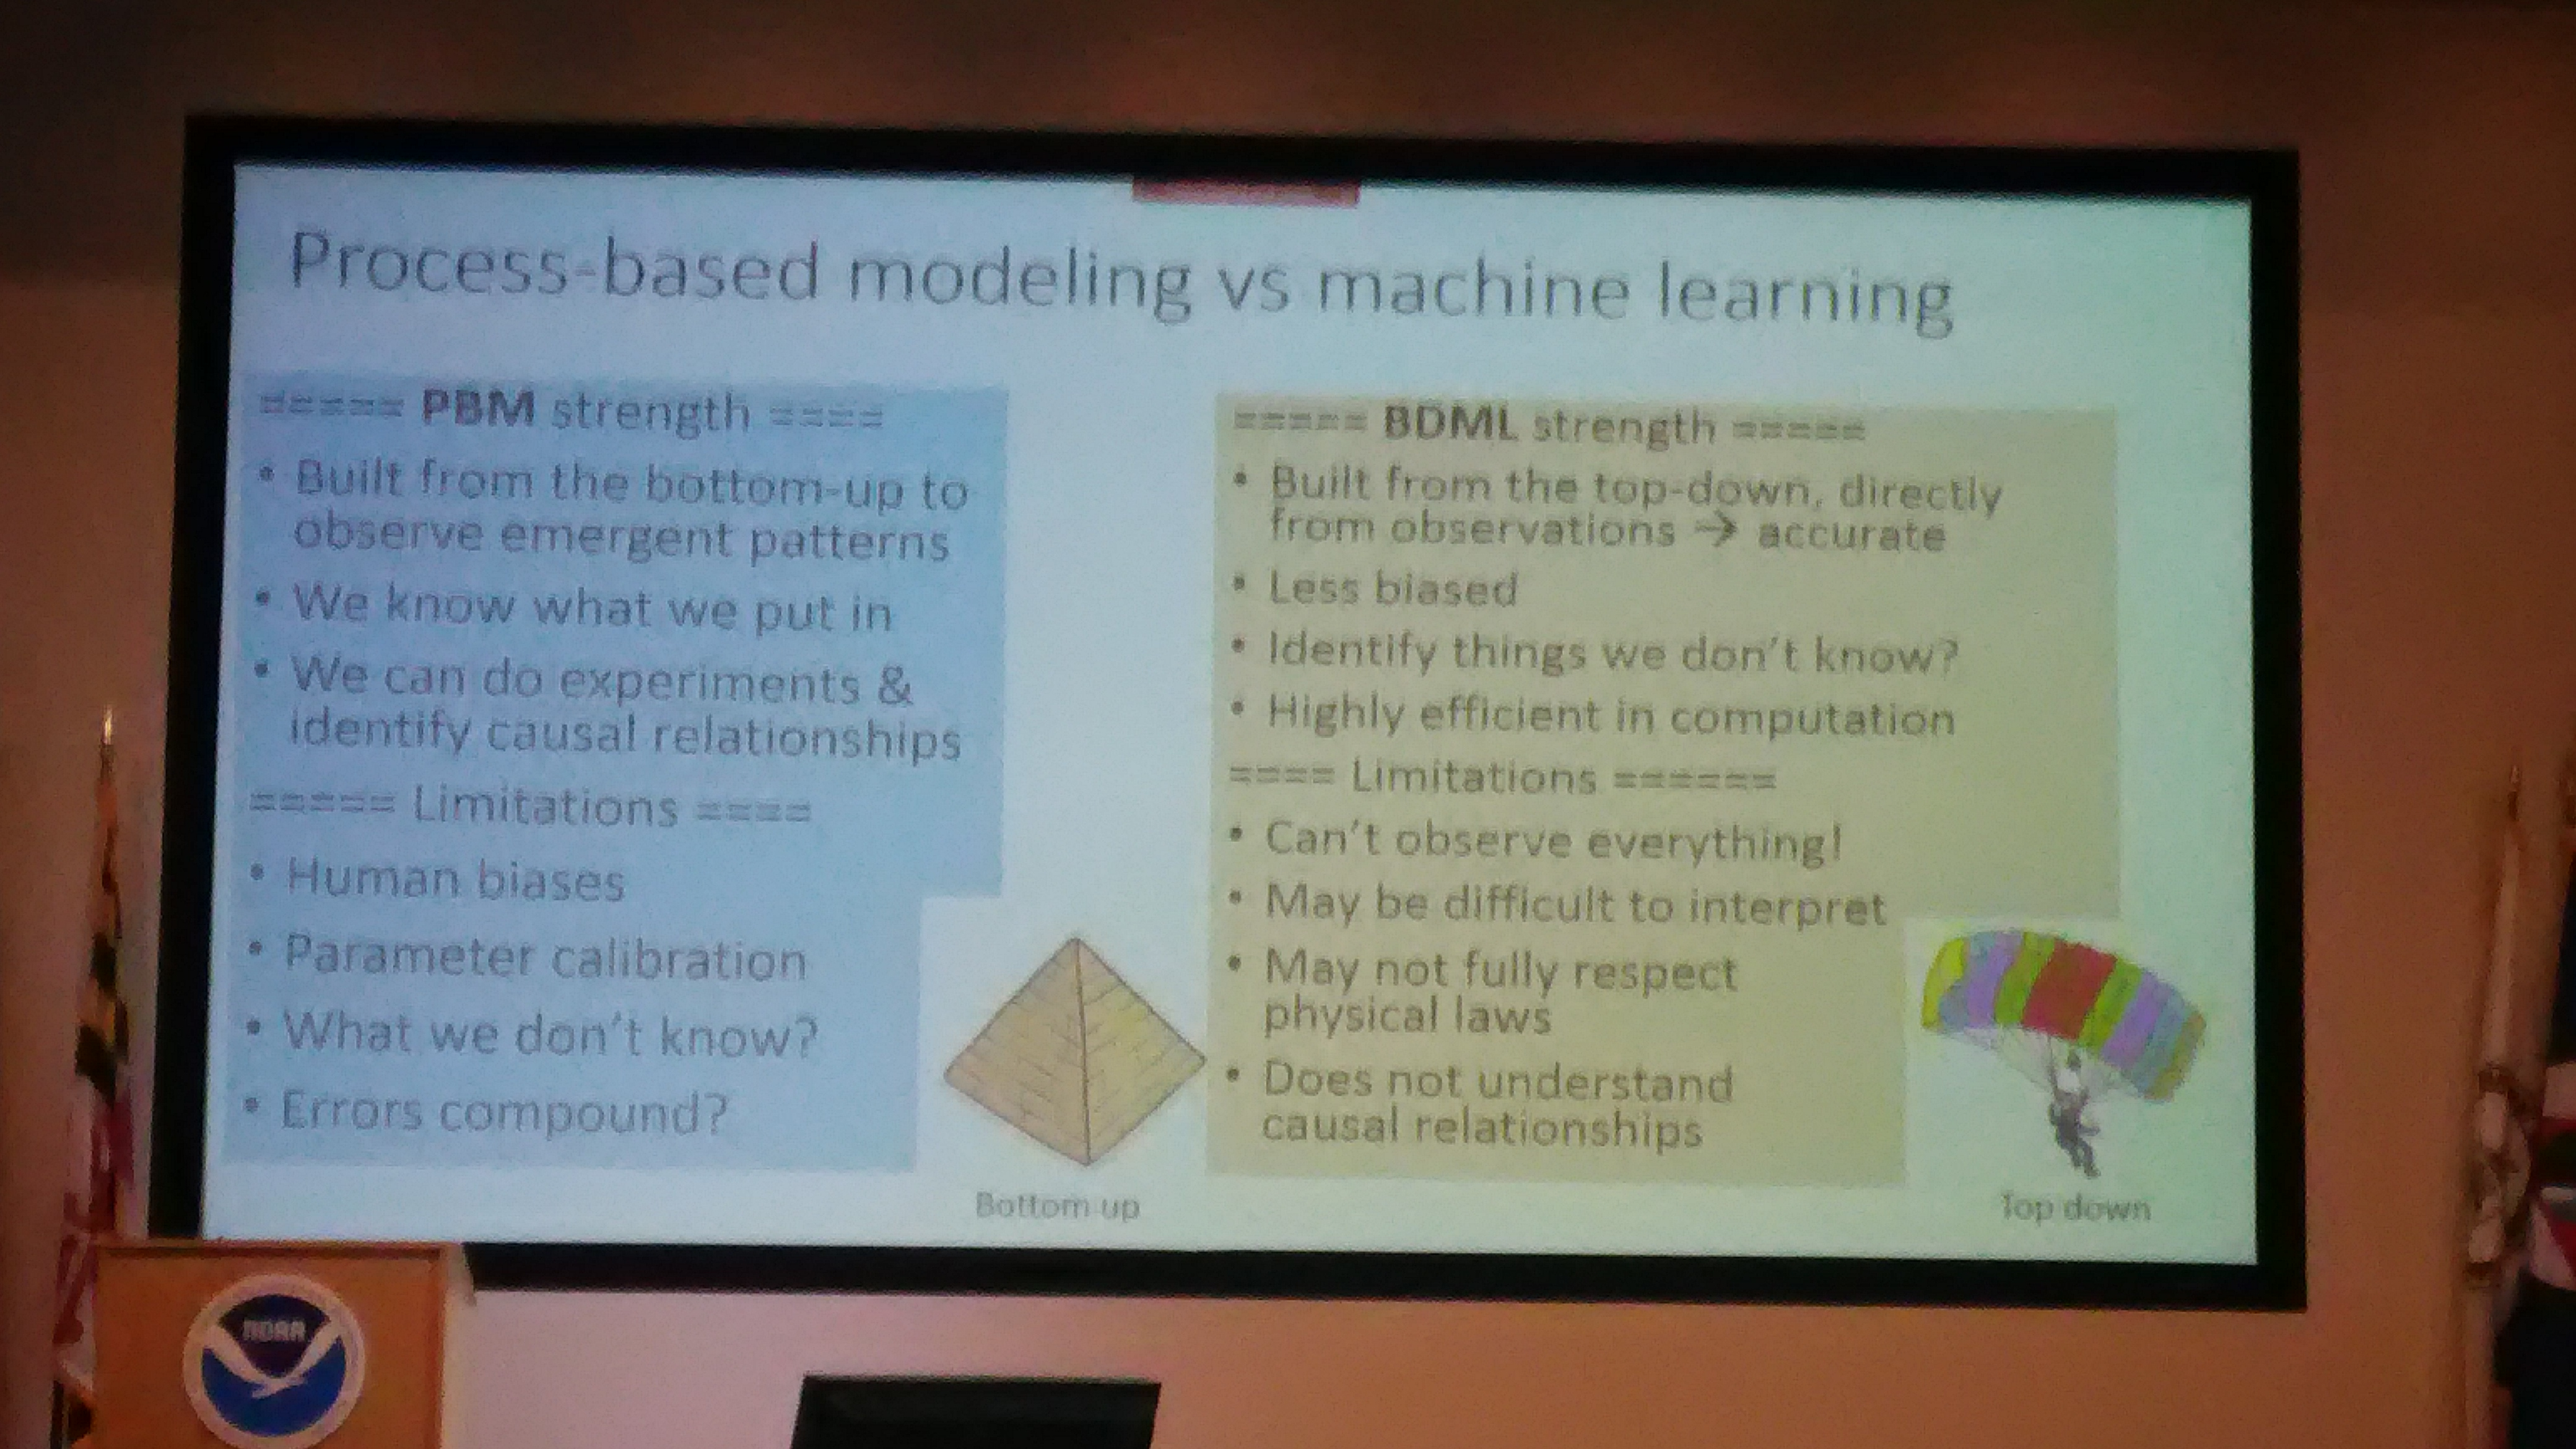
\includegraphics[width=.9\linewidth]{figs/P_20190424_114648.jpg}
\end{figure}
\end{frame}

\begin{frame}
\frametitle{Sid Boukabara, NOAA \textit{(Overview of NOAA AI activities in satellite obs. and NWP)}}
Data fusion + AI and physics
\begin{figure}
	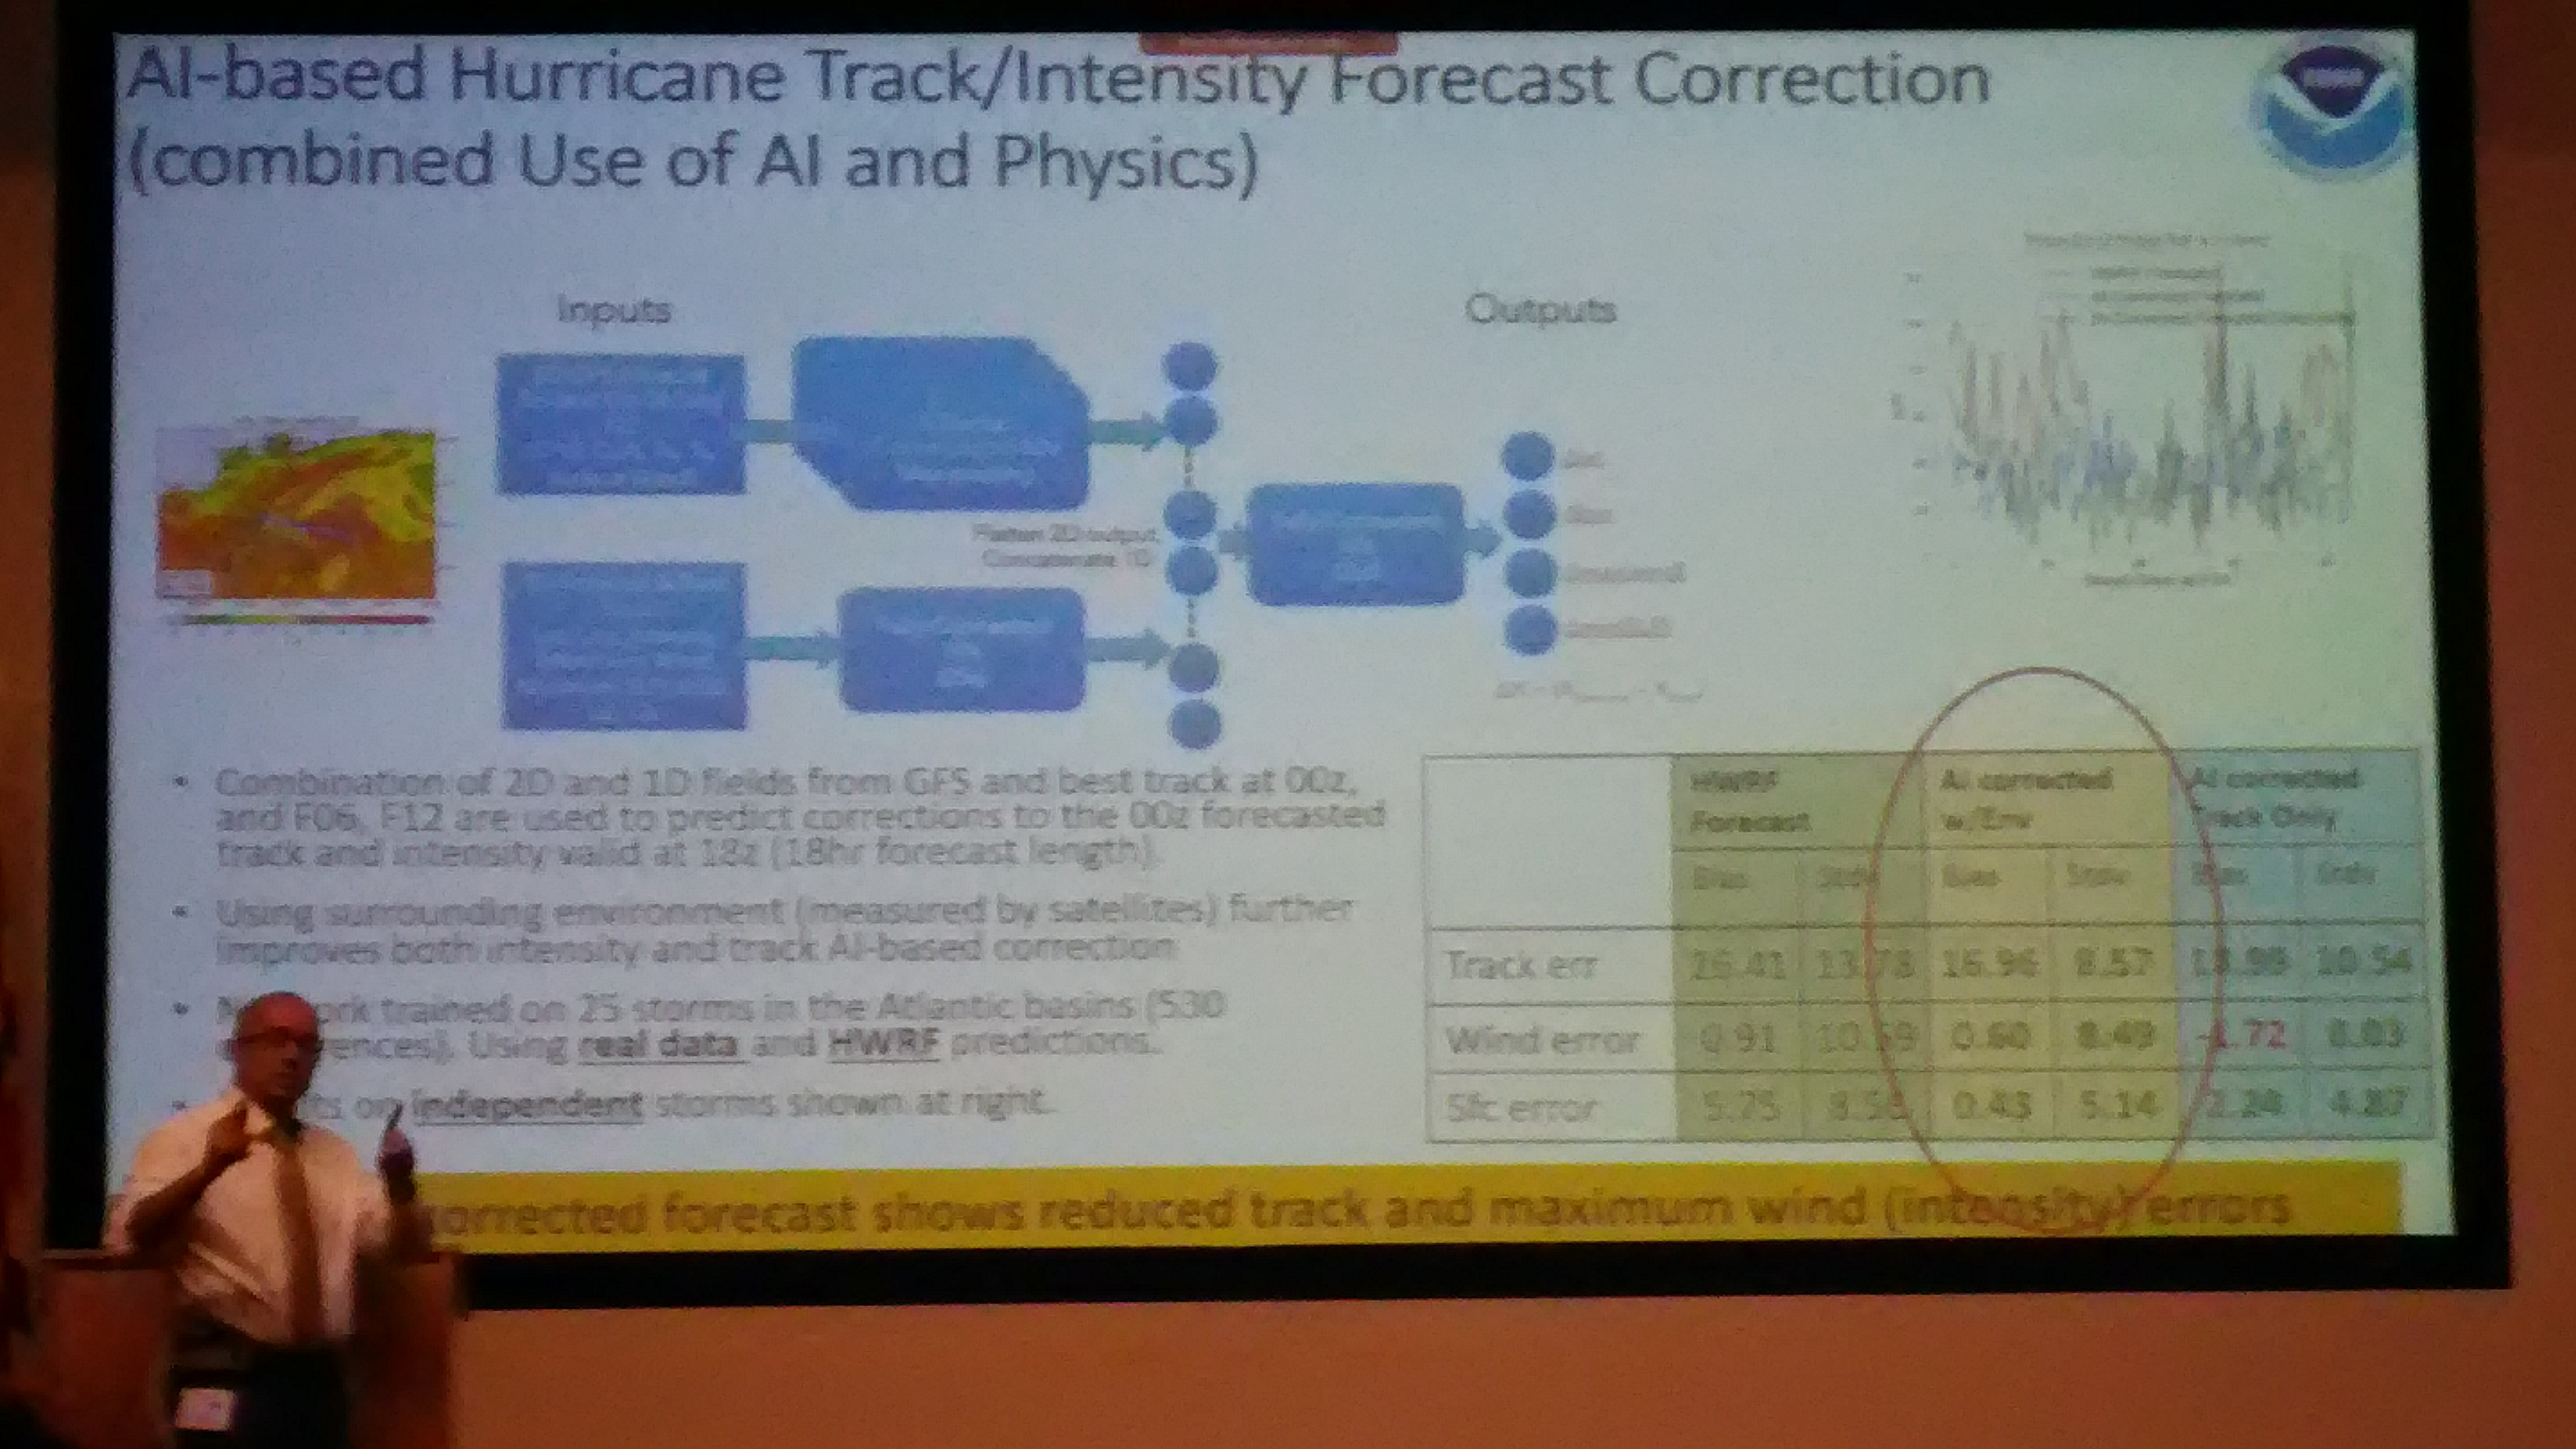
\includegraphics[width=.9\linewidth]{figs/P_20190423_111340.jpg}
\end{figure}
\end{frame}


\begin{frame}
\frametitle{Peter Jan van Leeuwen, Colorado State U. \textit{(Machine learning meets data assimilation)}}
\begin{figure}
	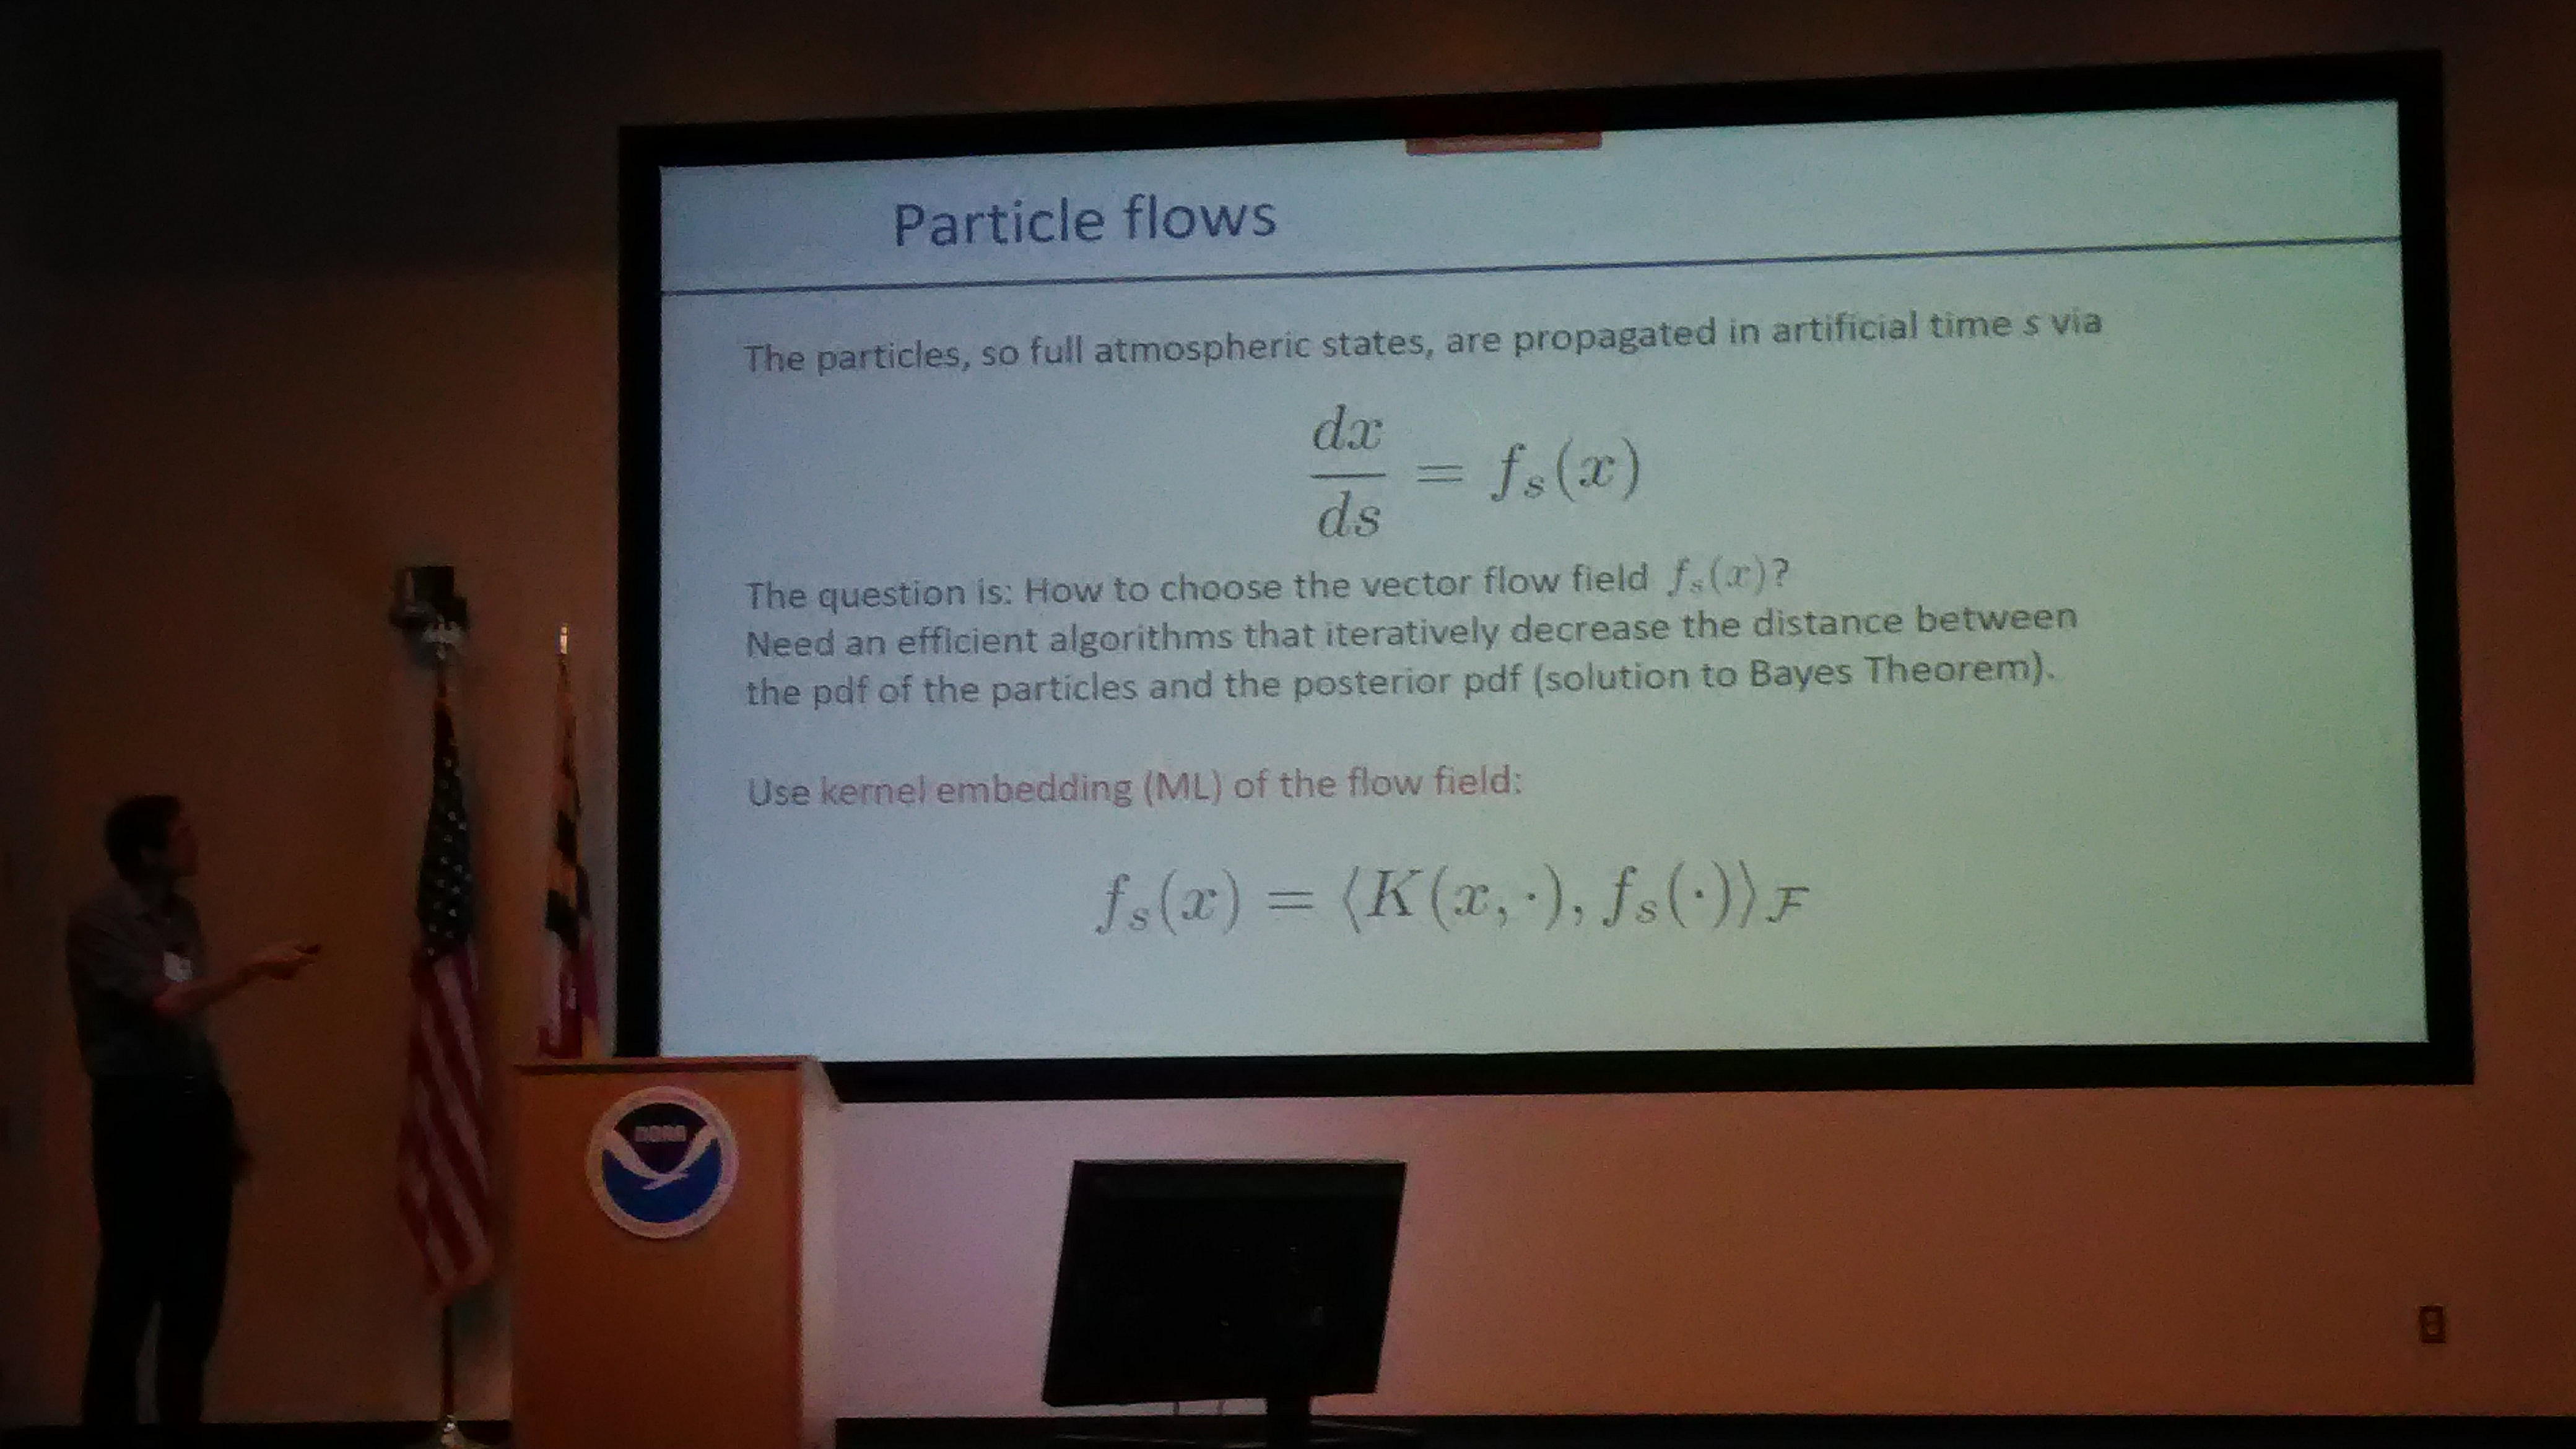
\includegraphics[width=.9\linewidth]{figs/P_20190424_142507.jpg}
\end{figure}
\end{frame}

\begin{frame}
\frametitle{Google, \textit{(Data driven discretization for partial differential equations)}}
github.com/google/pde-superresolution
\begin{figure}
	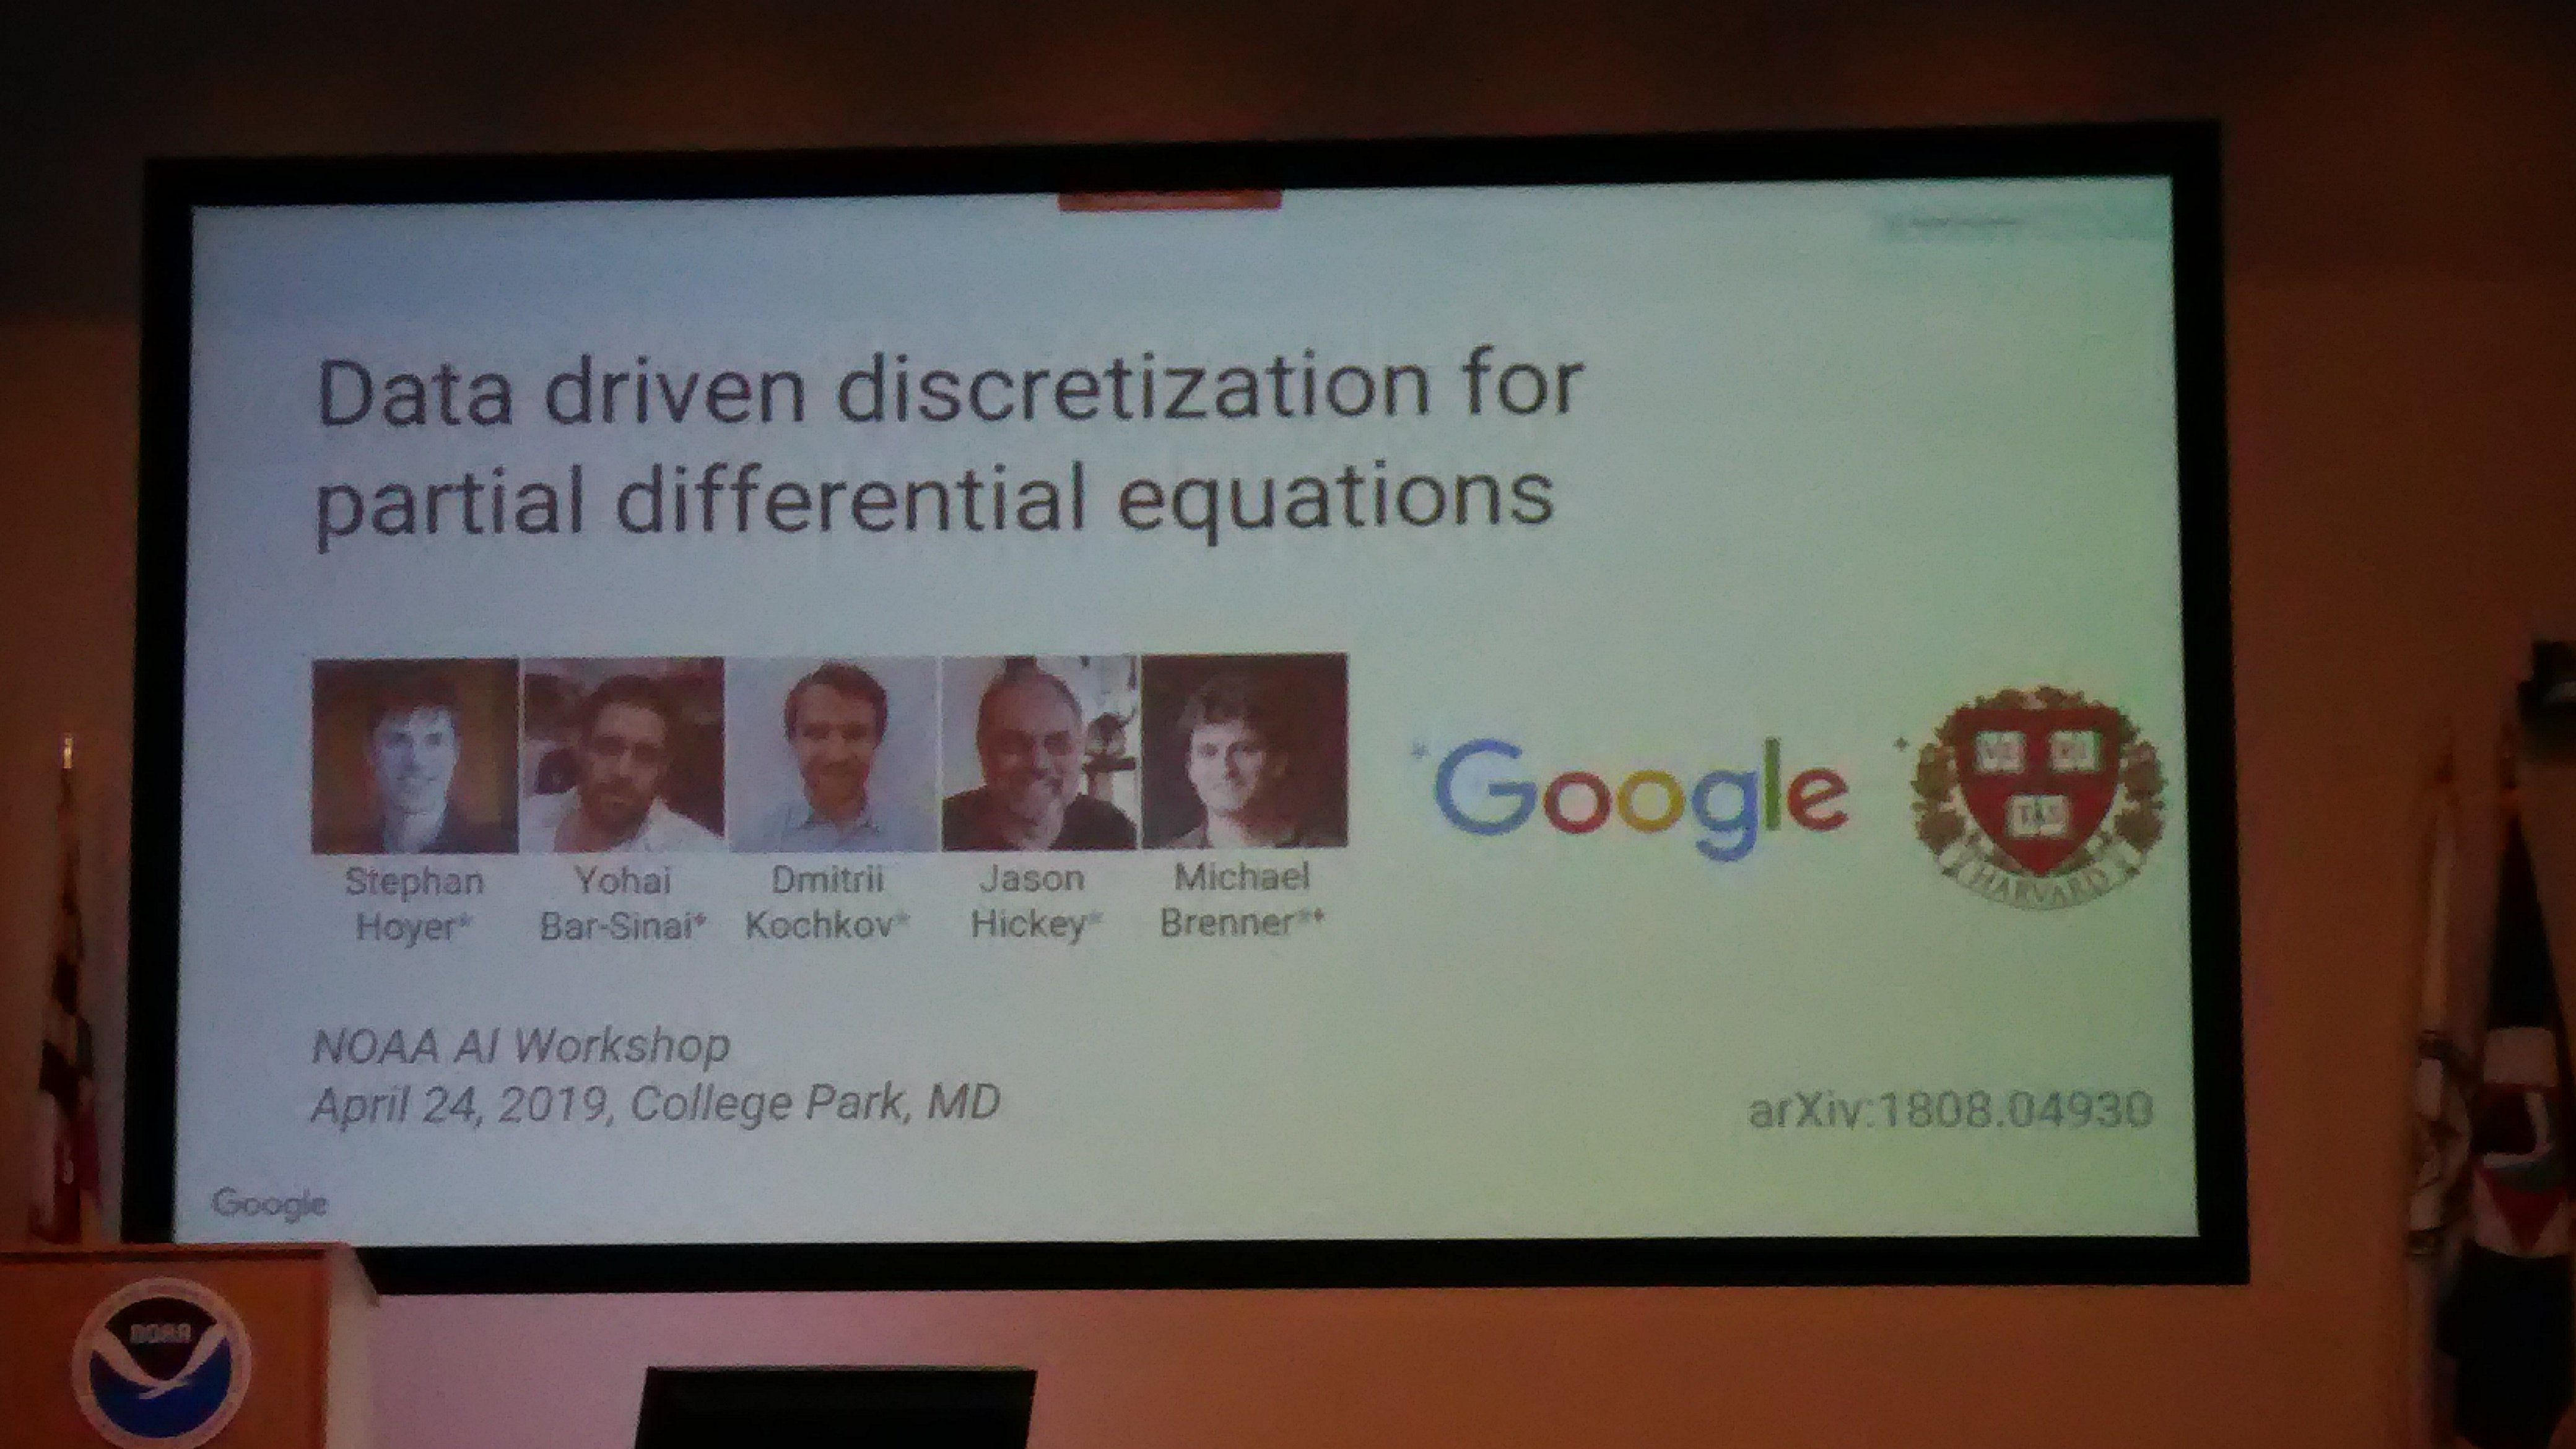
\includegraphics[width=.9\linewidth]{figs/P_20190424_153531.jpg}
\end{figure}
\end{frame}

\begin{frame}
\frametitle{Google, \textit{(Data driven discretization for partial differential equations)}}
github.com/google/pde-superresolution
\begin{figure}
	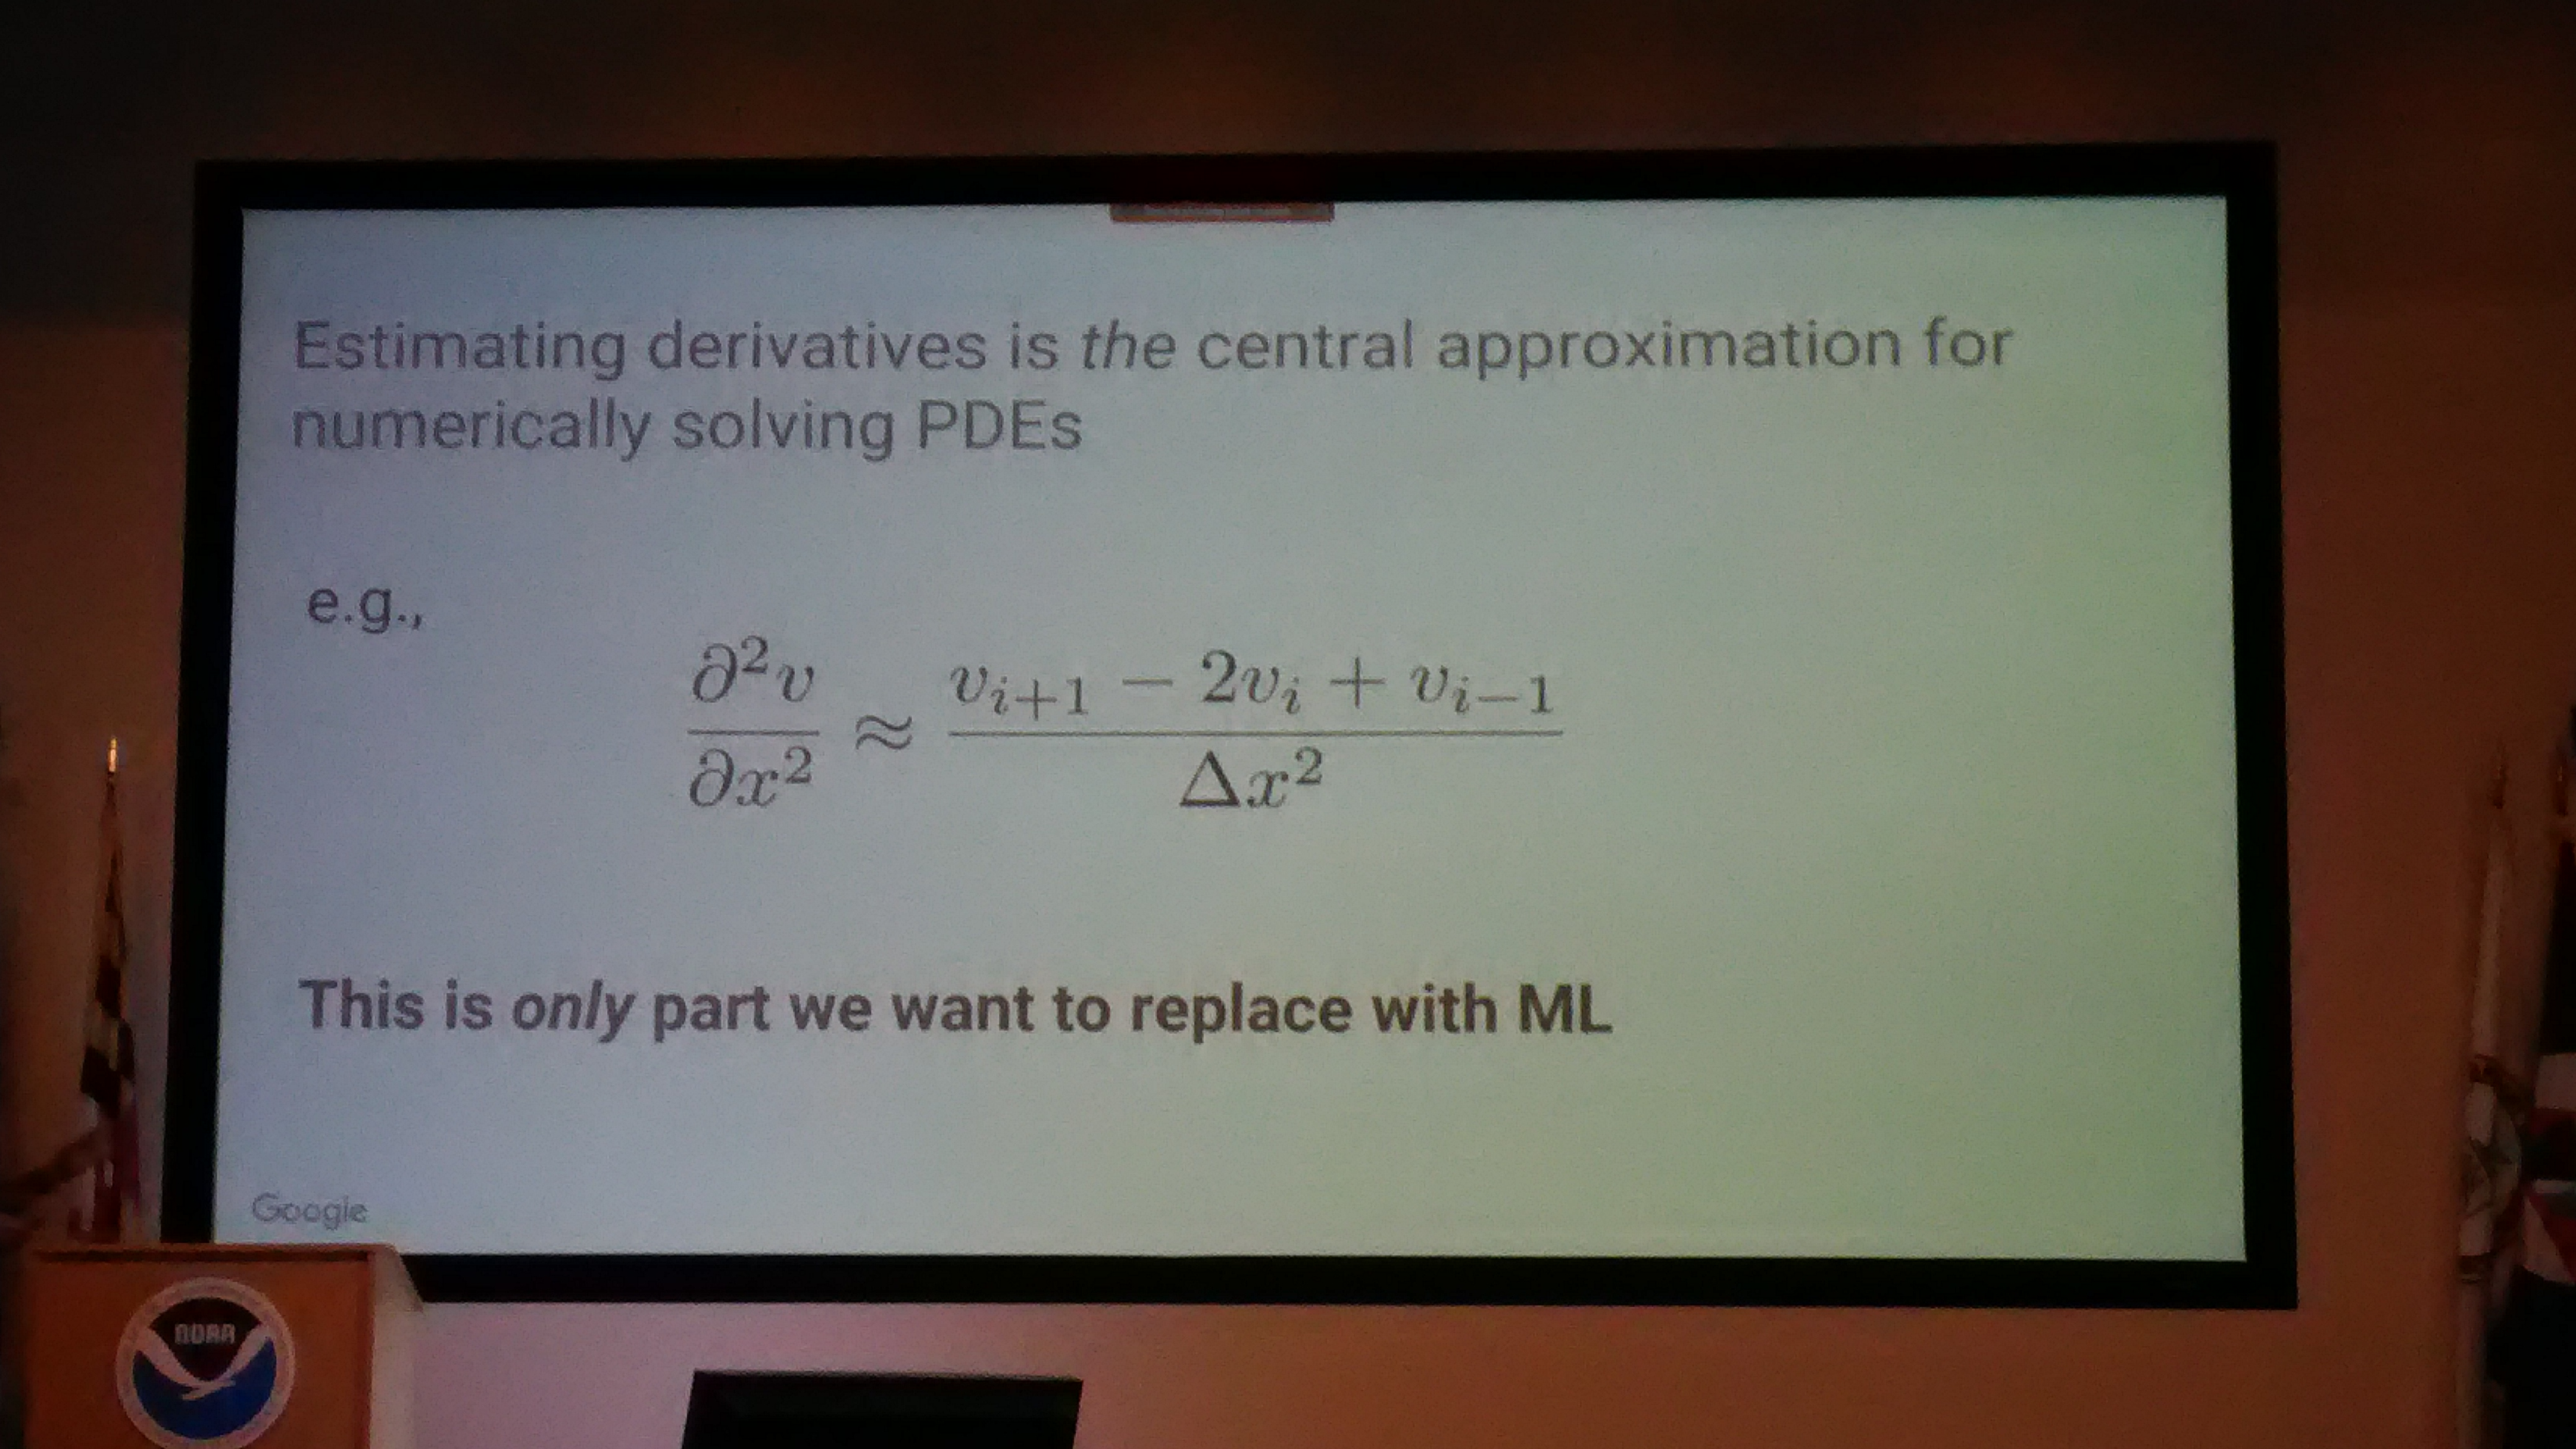
\includegraphics[width=.9\linewidth]{figs/P_20190424_154437.jpg}
\end{figure}
\end{frame}

\begin{frame}
\frametitle{Google, \textit{(Data driven discretization for partial differential equations)}}
github.com/google/pde-superresolution
\begin{figure}
	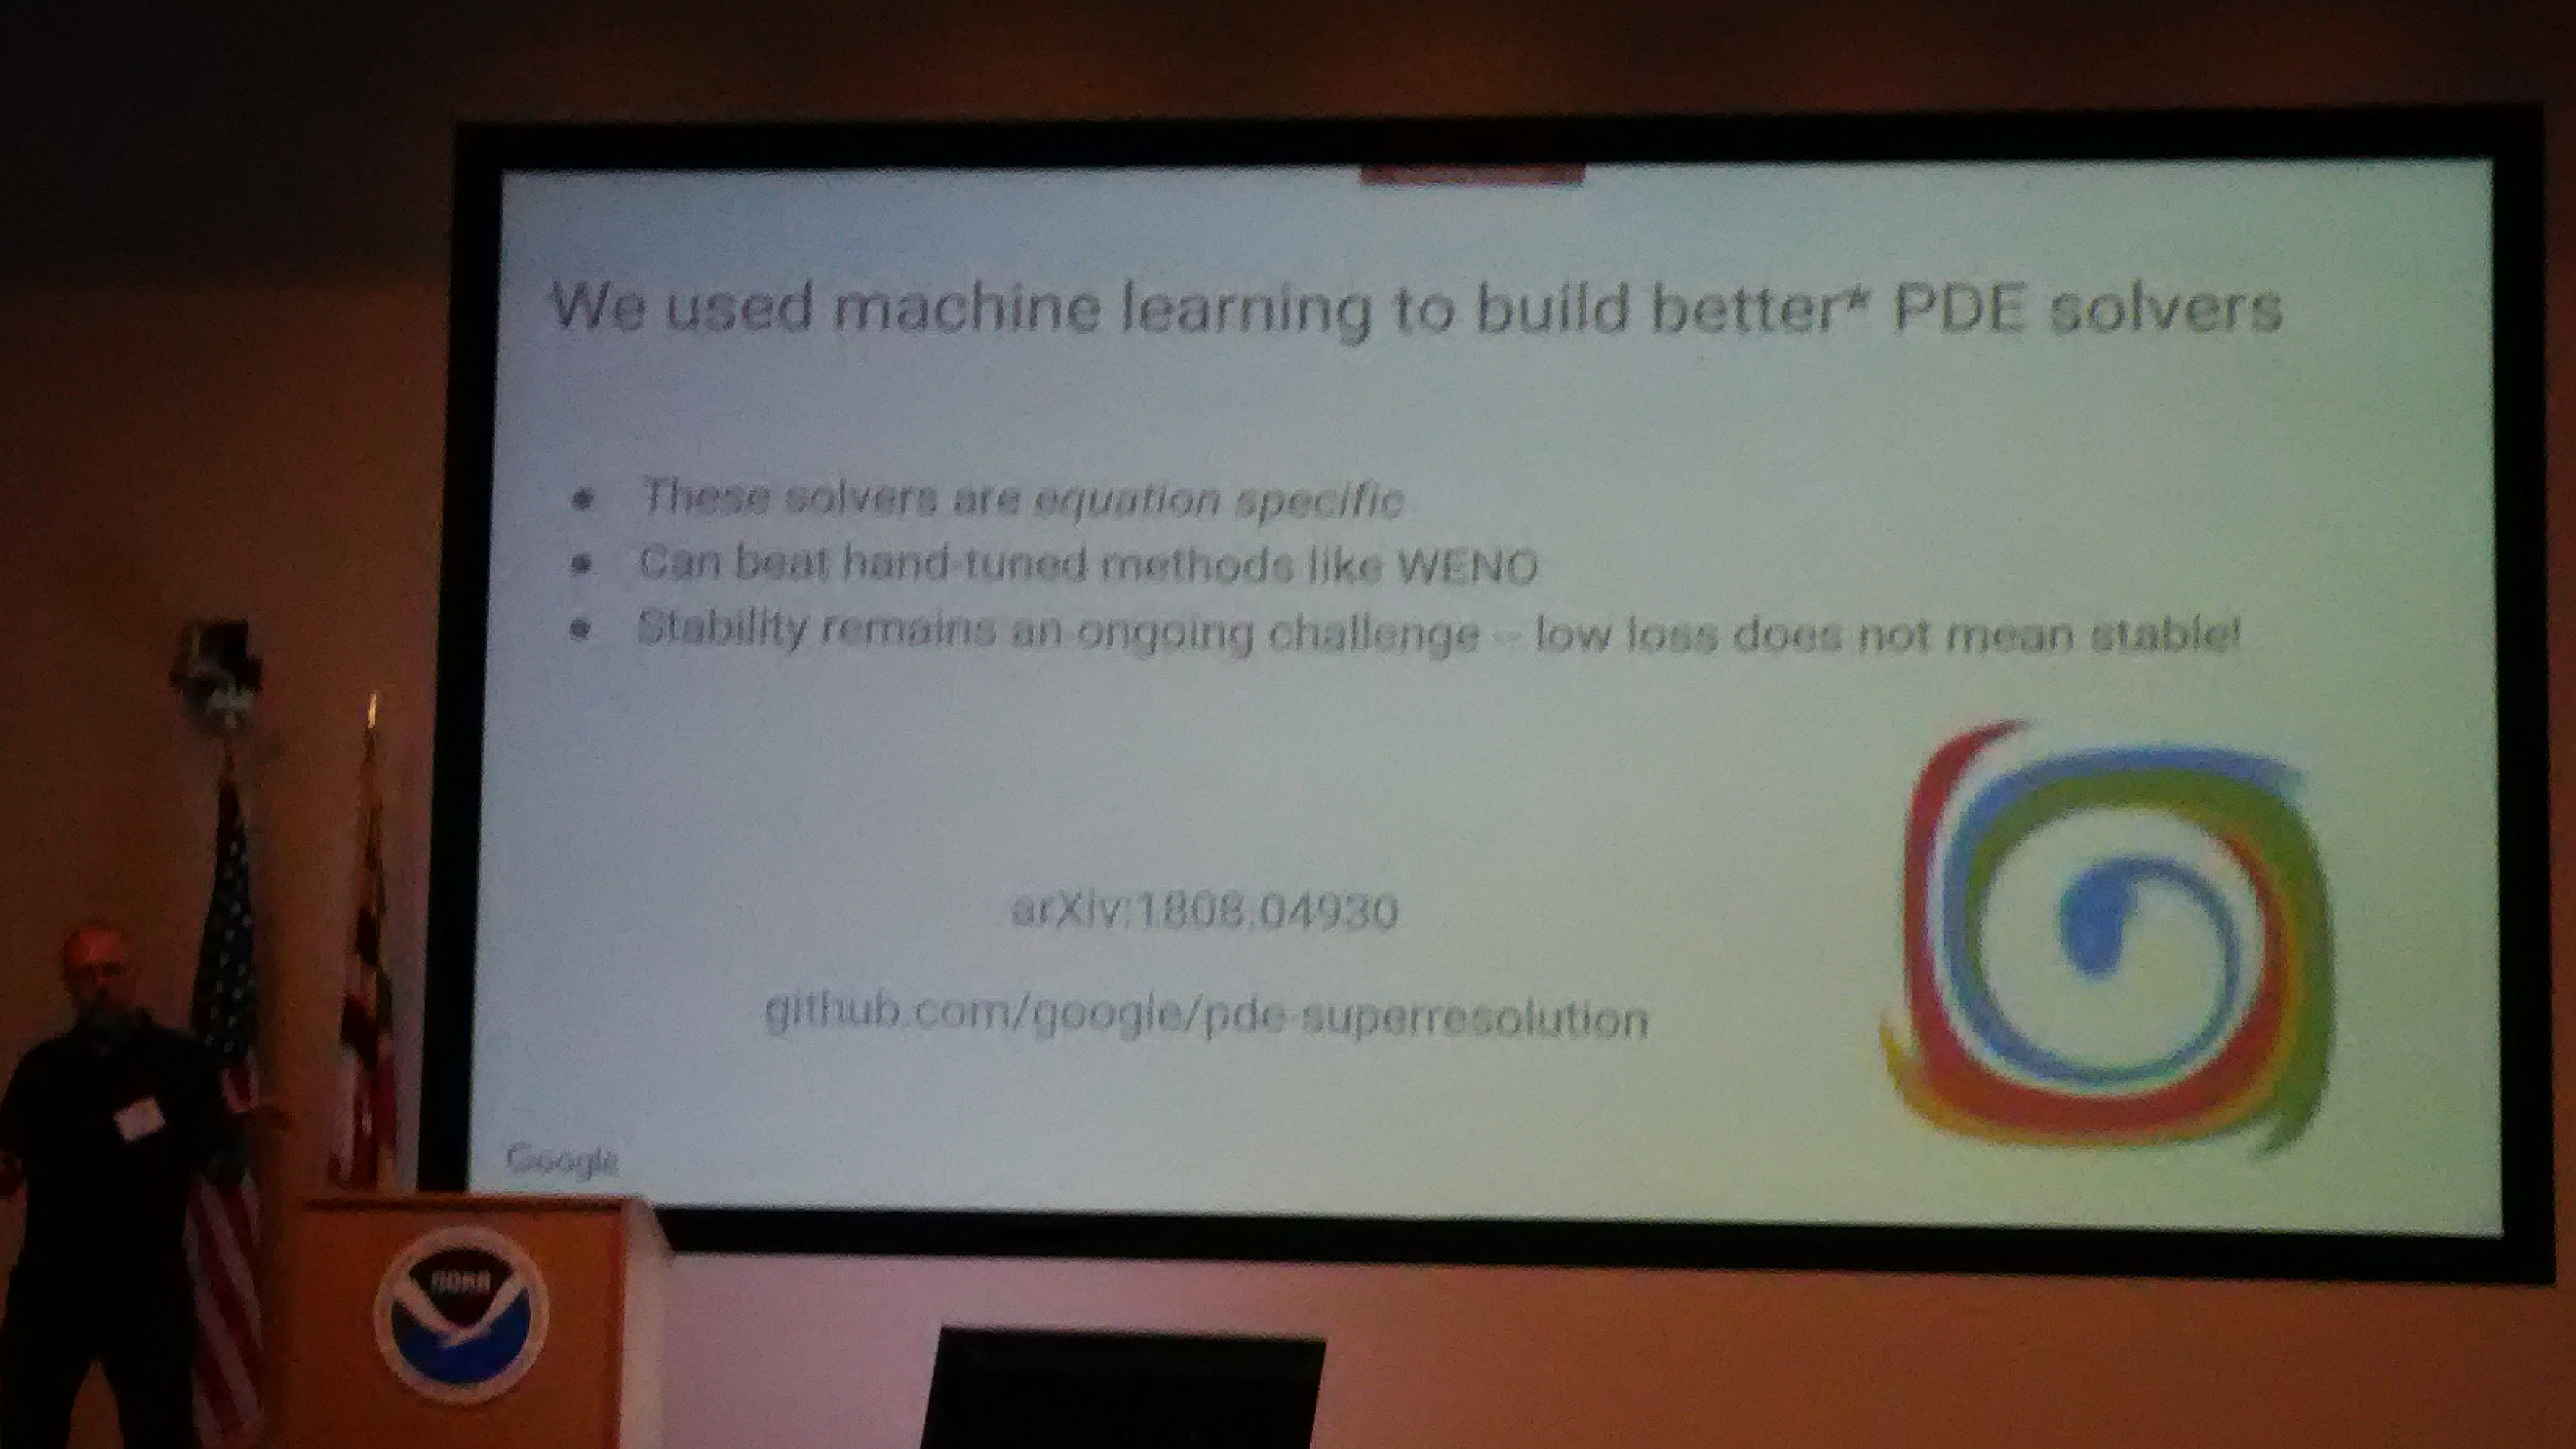
\includegraphics[width=.9\linewidth]{figs/P_20190424_155240.jpg}
\end{figure}
\end{frame}

\begin{frame}
\frametitle{Google, \textit{(Data driven discretization for partial differential equations)}}
github.com/google/pde-superresolution
\begin{figure}
	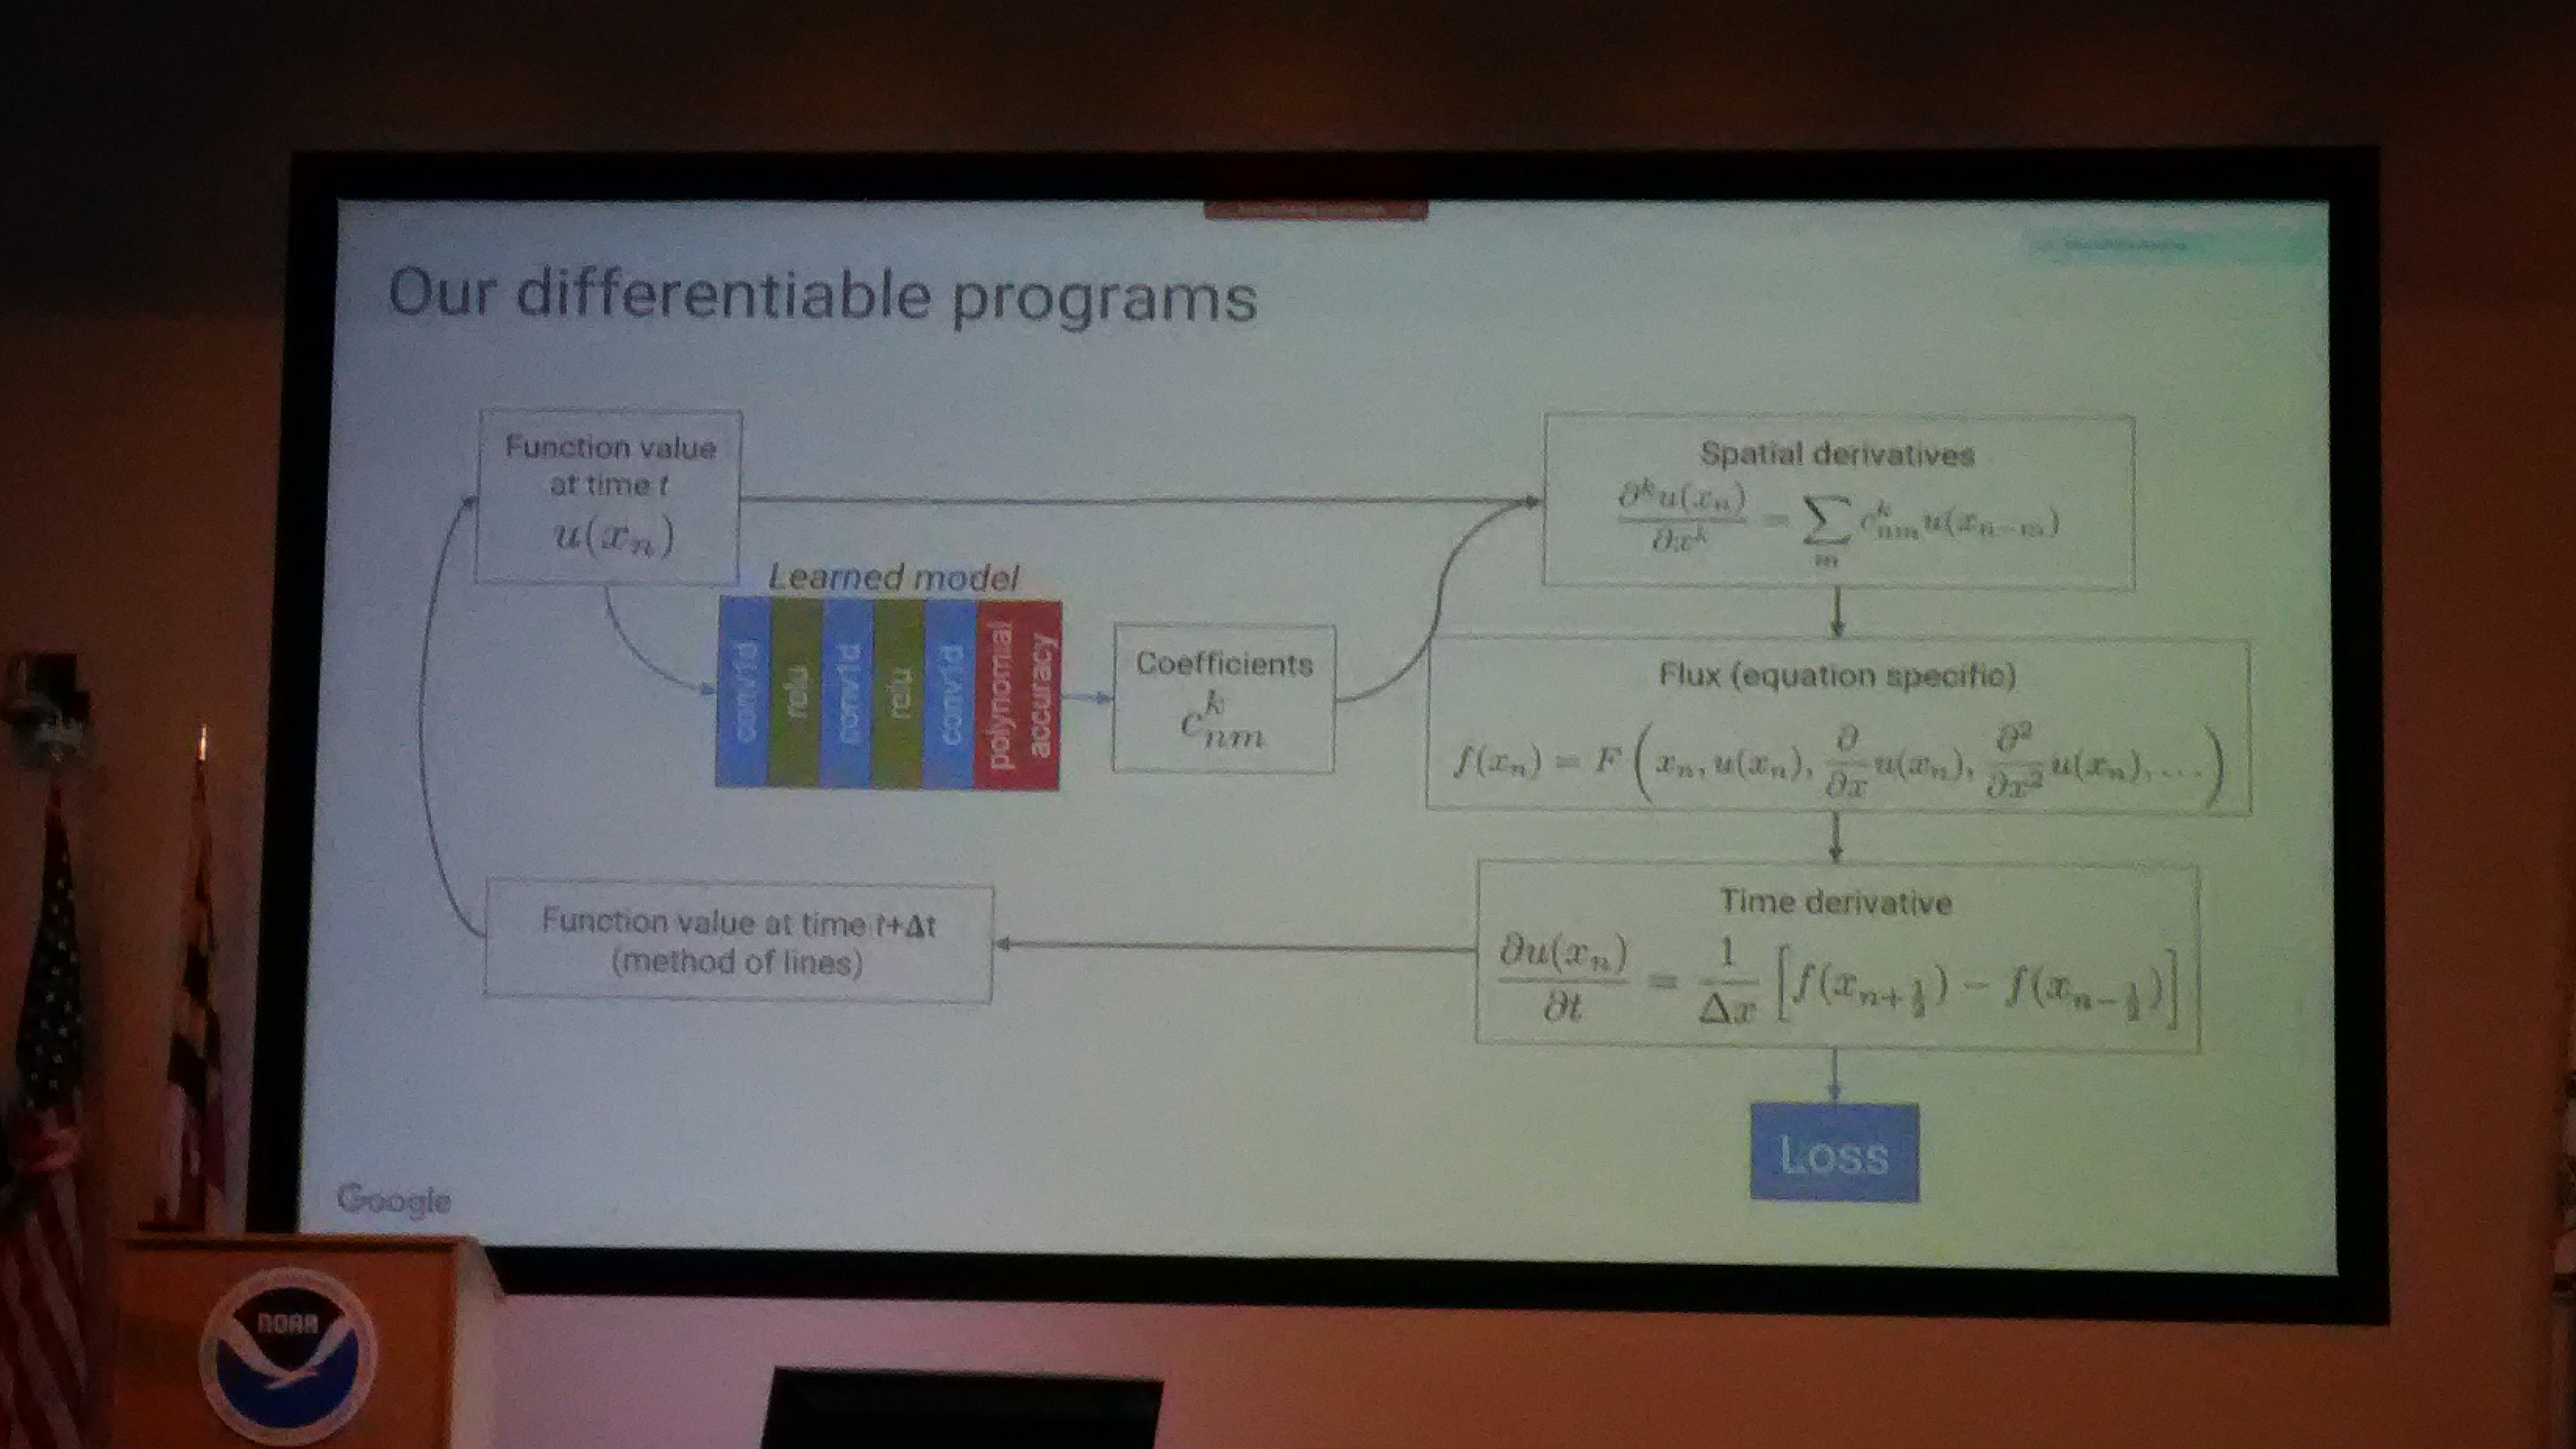
\includegraphics[width=.9\linewidth]{figs/P_20190424_155515.jpg}
\end{figure}
\end{frame}

\subsection{Applications}

\begin{frame}
\frametitle{Outline} % Table of contents slide, comment this block out to remove it
\tableofcontents[currentsection] % Throughout your presentation, if you choose to use \section{} and \subsection{} commands, these will automatically be printed on this slide as an overview of your presentation
\end{frame}

\begin{frame}
\frametitle{Pamela Collins, Conservation International \textit{(AI for water infrastructure mapping in Africa)}}
\begin{figure}
	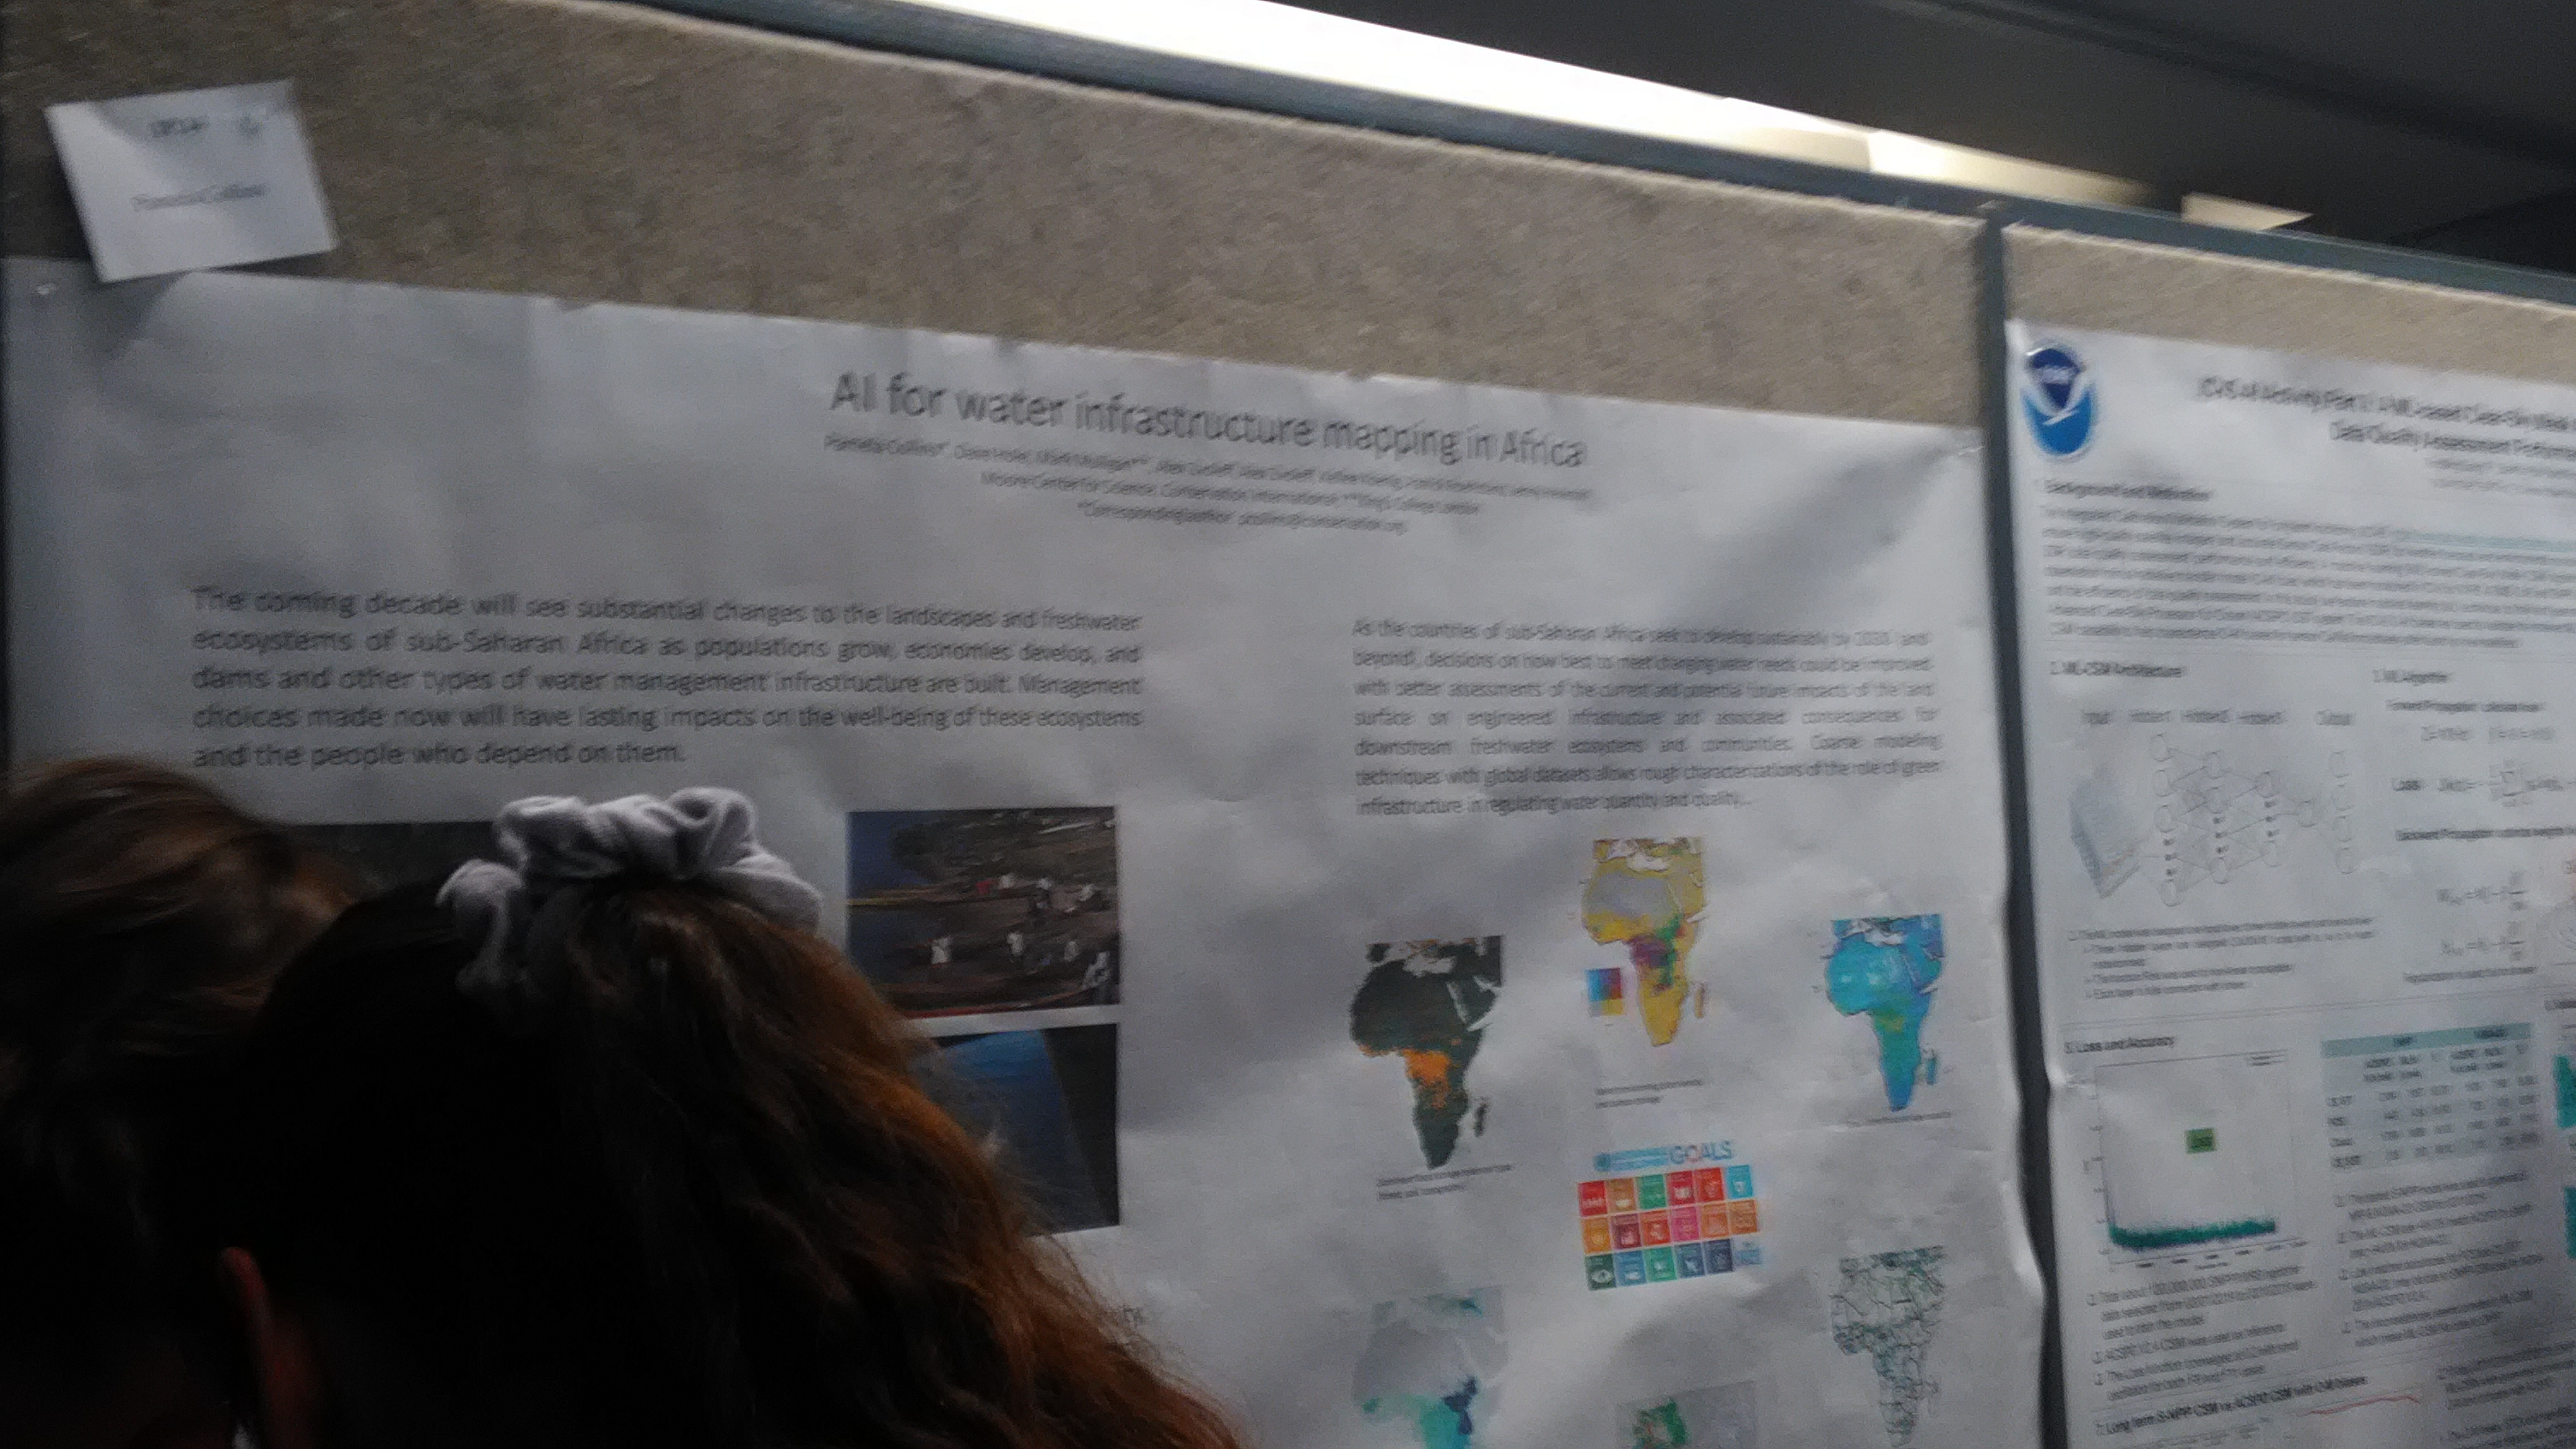
\includegraphics[width=.9\linewidth]{figs/P_20190423_143522.jpg}
\end{figure}
\end{frame}


\begin{frame}
\frametitle{Sean Helfrich, NOAA/NESDIS \textit{(Development of CNN for Ice and Flood Detection from Synthetic Aperture Radar)}}
\begin{figure}
	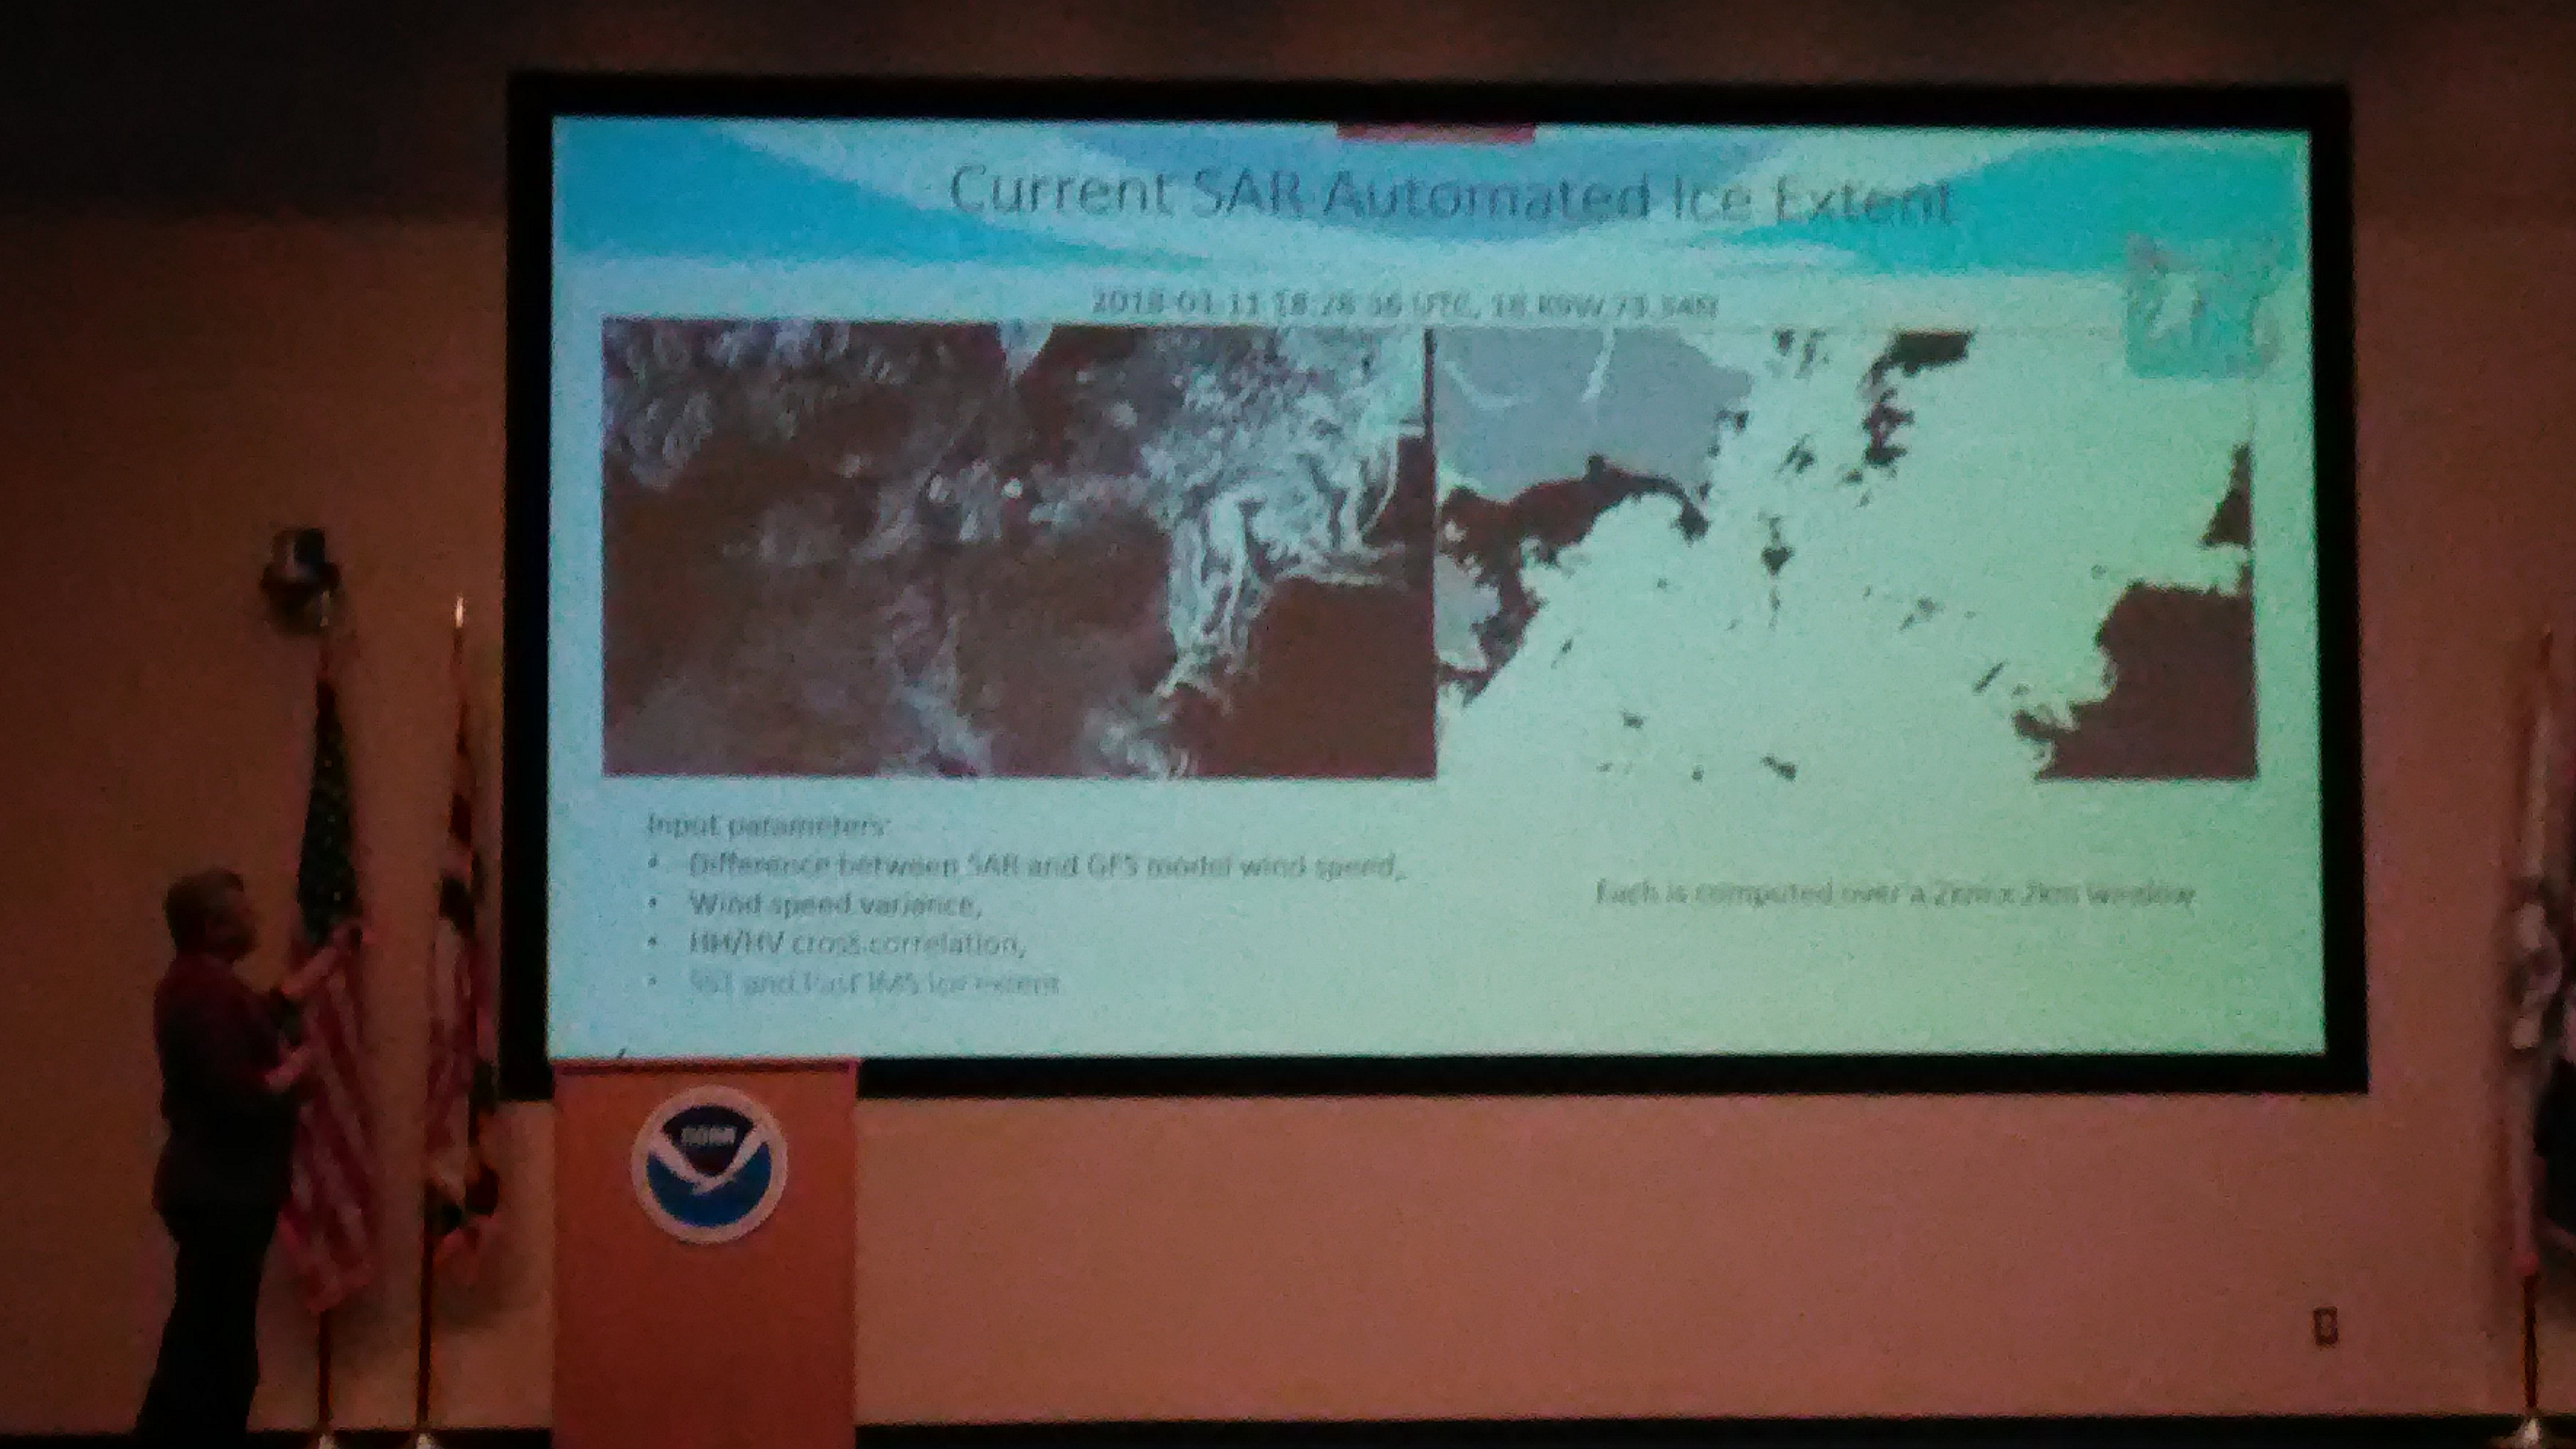
\includegraphics[width=.9\linewidth]{figs/P_20190423_155509.jpg}
\end{figure}
\end{frame}


\begin{frame}
\frametitle{Christina Kumler, NOAA Boulder \textit{(Using DL to extract regions of interest from satellite data)}}
\begin{figure}
	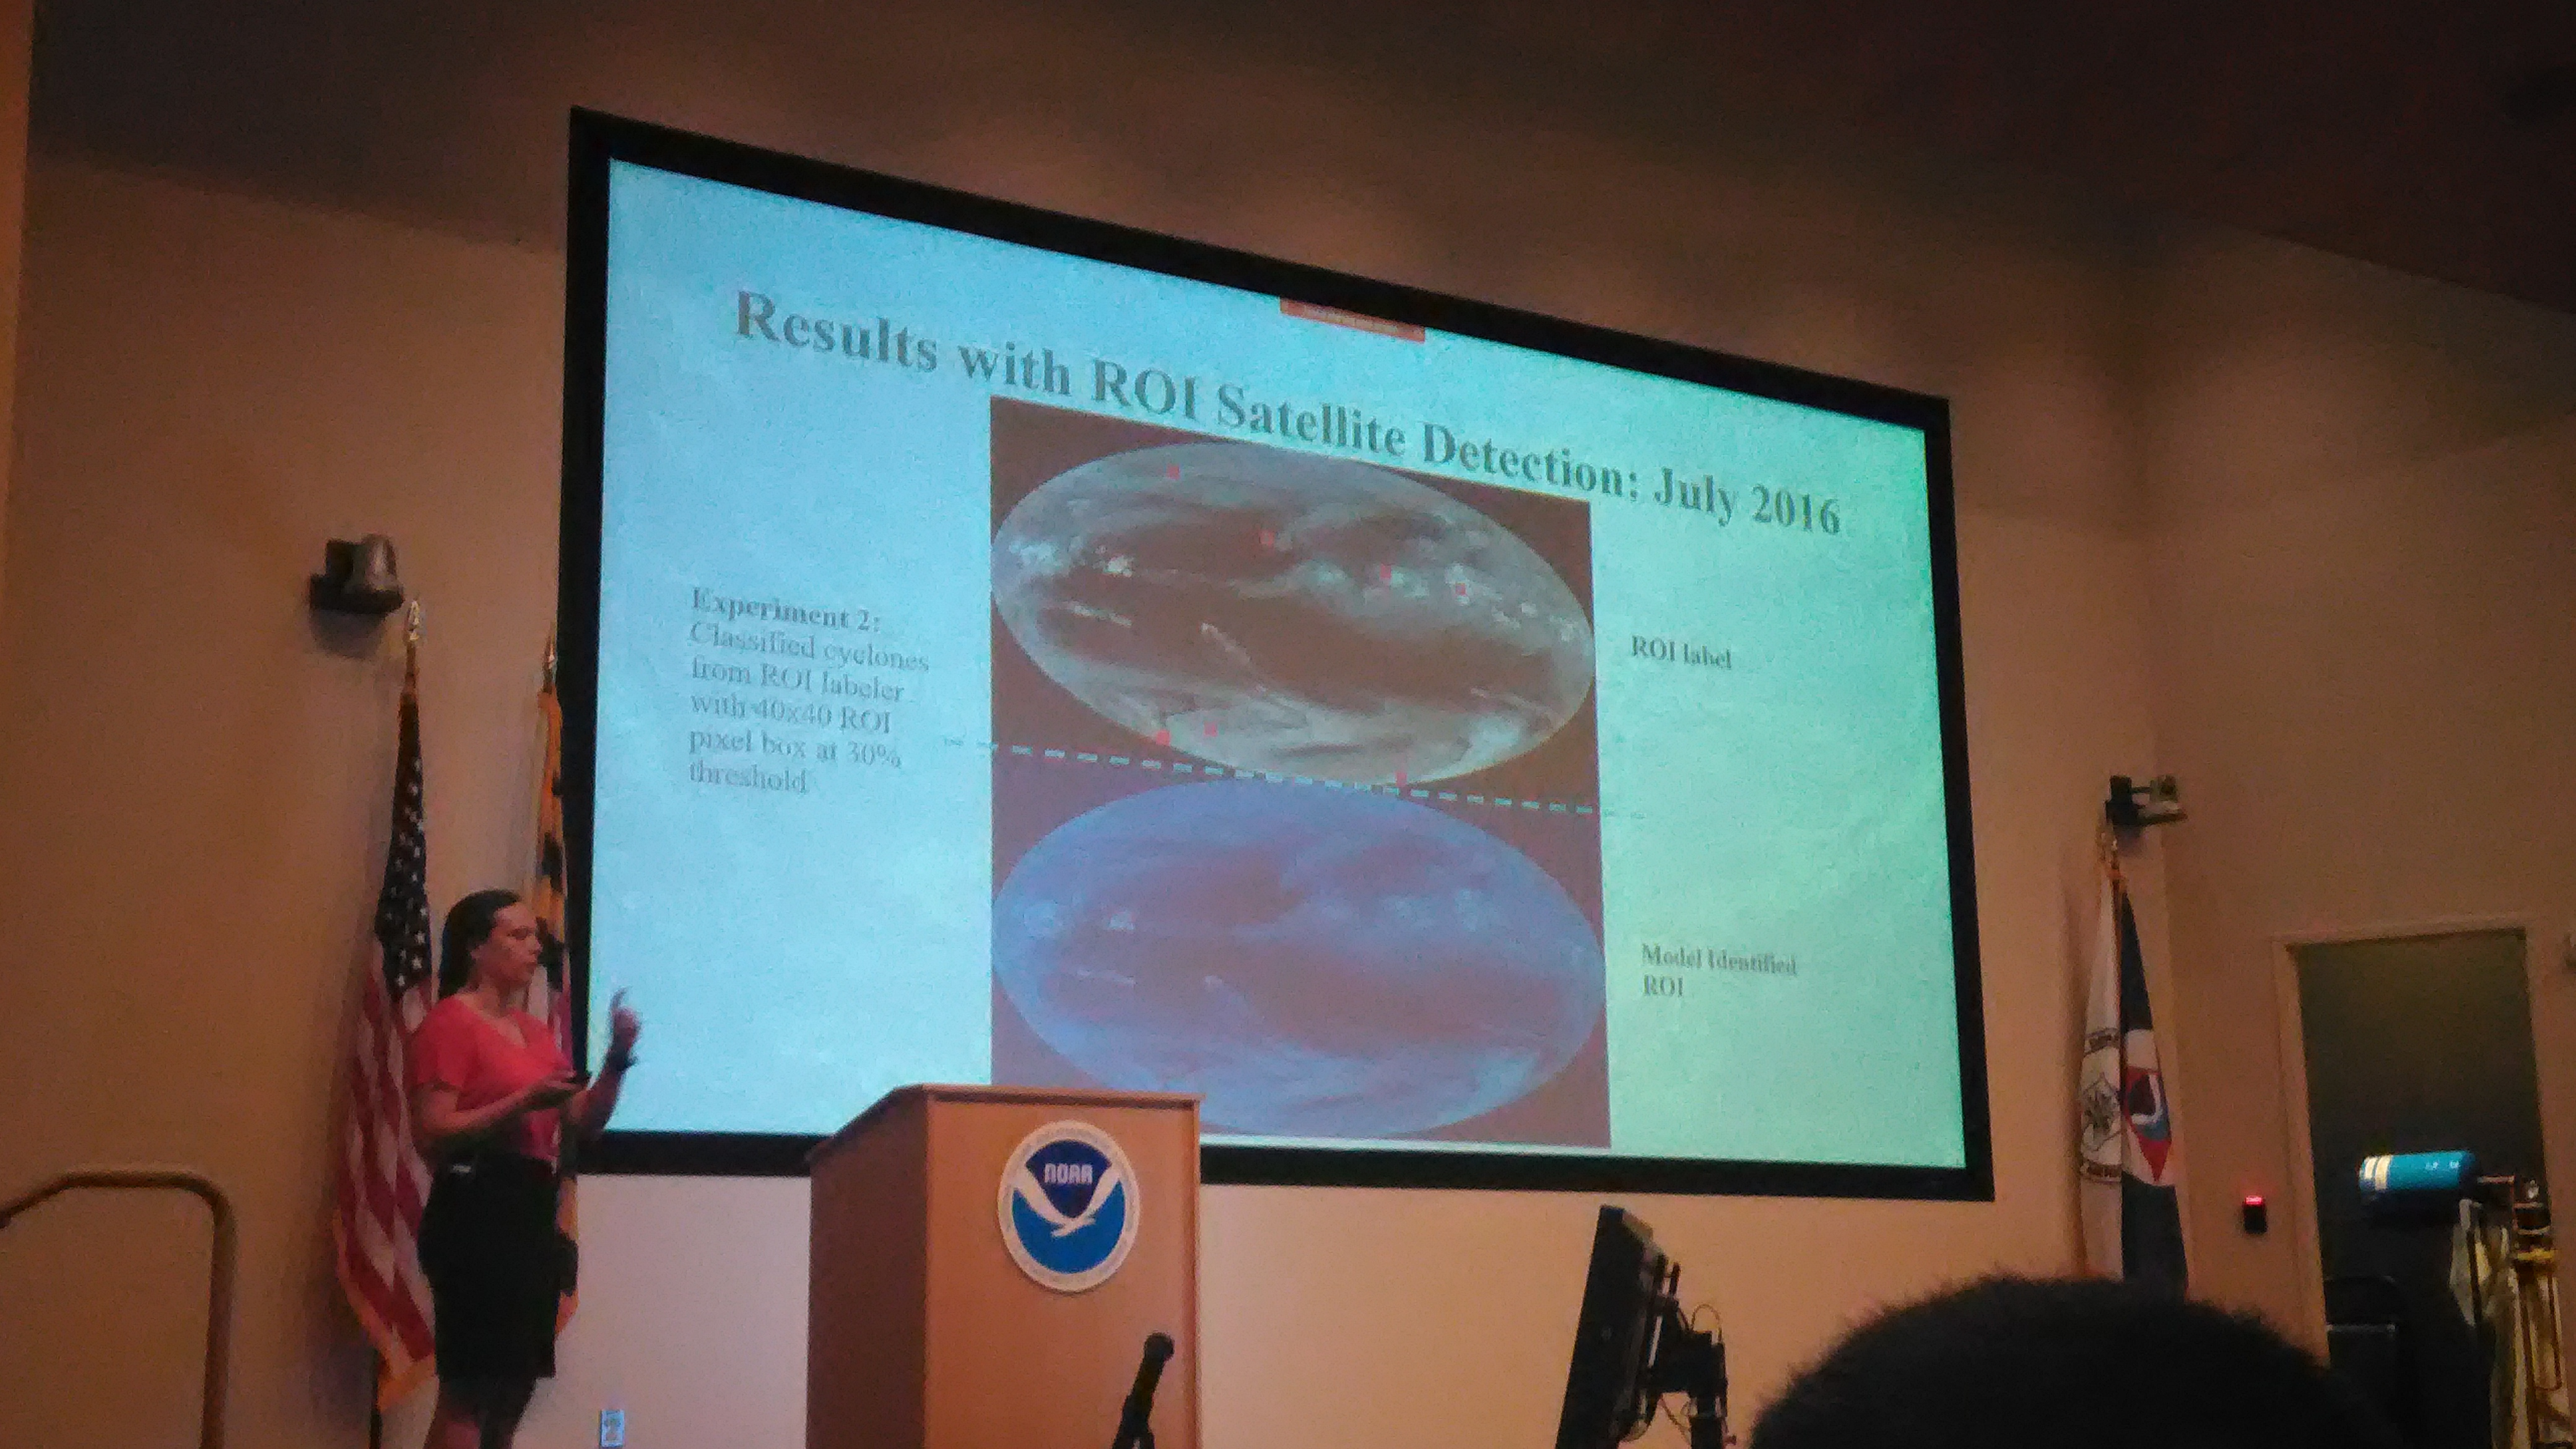
\includegraphics[width=.9\linewidth]{figs/P_20190424_092340.jpg}
\end{figure}
\end{frame}

\begin{frame}
\frametitle{Alexandra Grimes, MSU \textit{(Atlantic basin rapid intensification prediction enhancement through NWP spatial information)}}
\begin{figure}
	\includegraphics[width=.9\linewidth]{figs/P_20190424_102707.jpg}
\end{figure}
\end{frame}

\begin{frame}
\frametitle{Narges Shahroudi, RTi for NOAA/NESDIS \textit{(Improvement to hurricane track and intensity forecast by exploiting satellite dat and ML.)}}
\begin{figure}
	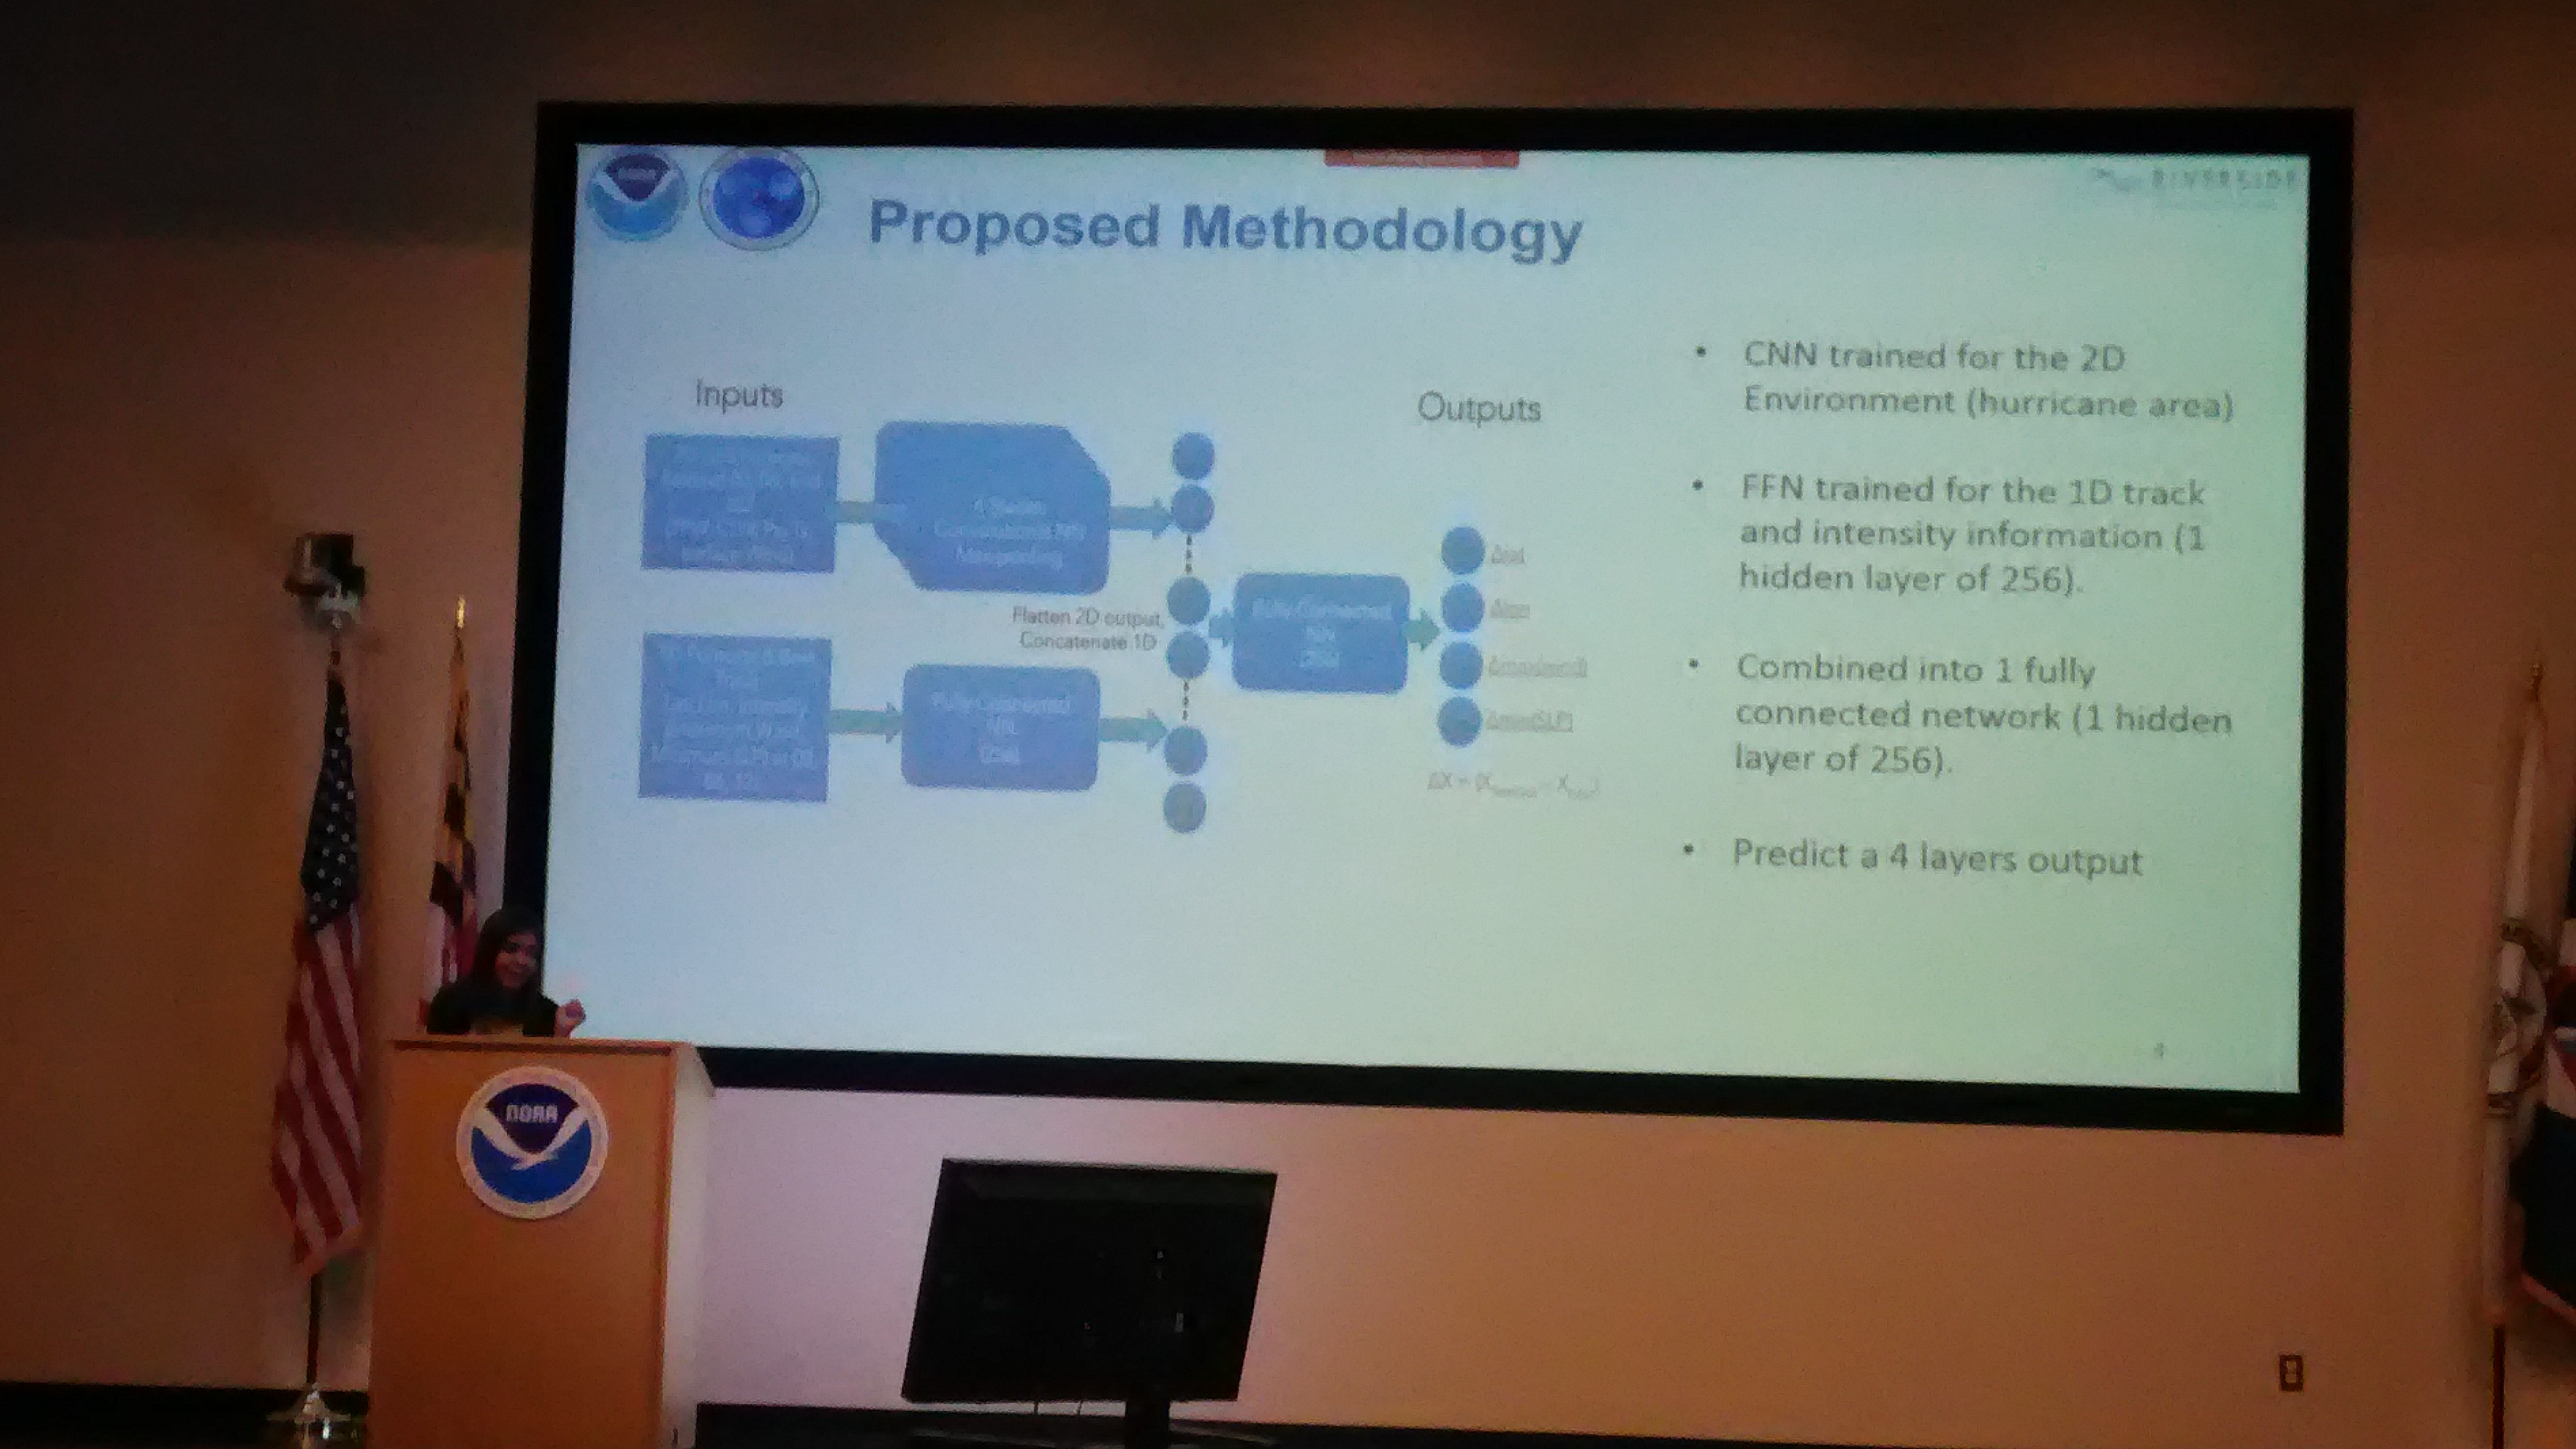
\includegraphics[width=.9\linewidth]{figs/P_20190424_143519.jpg}
\end{figure}
\end{frame}

\begin{frame}
\frametitle{Christoph Keller, NASA/GMAO \textit{(Atmospheric chemistry and air forecasting using machine learning)}}
\begin{figure}
	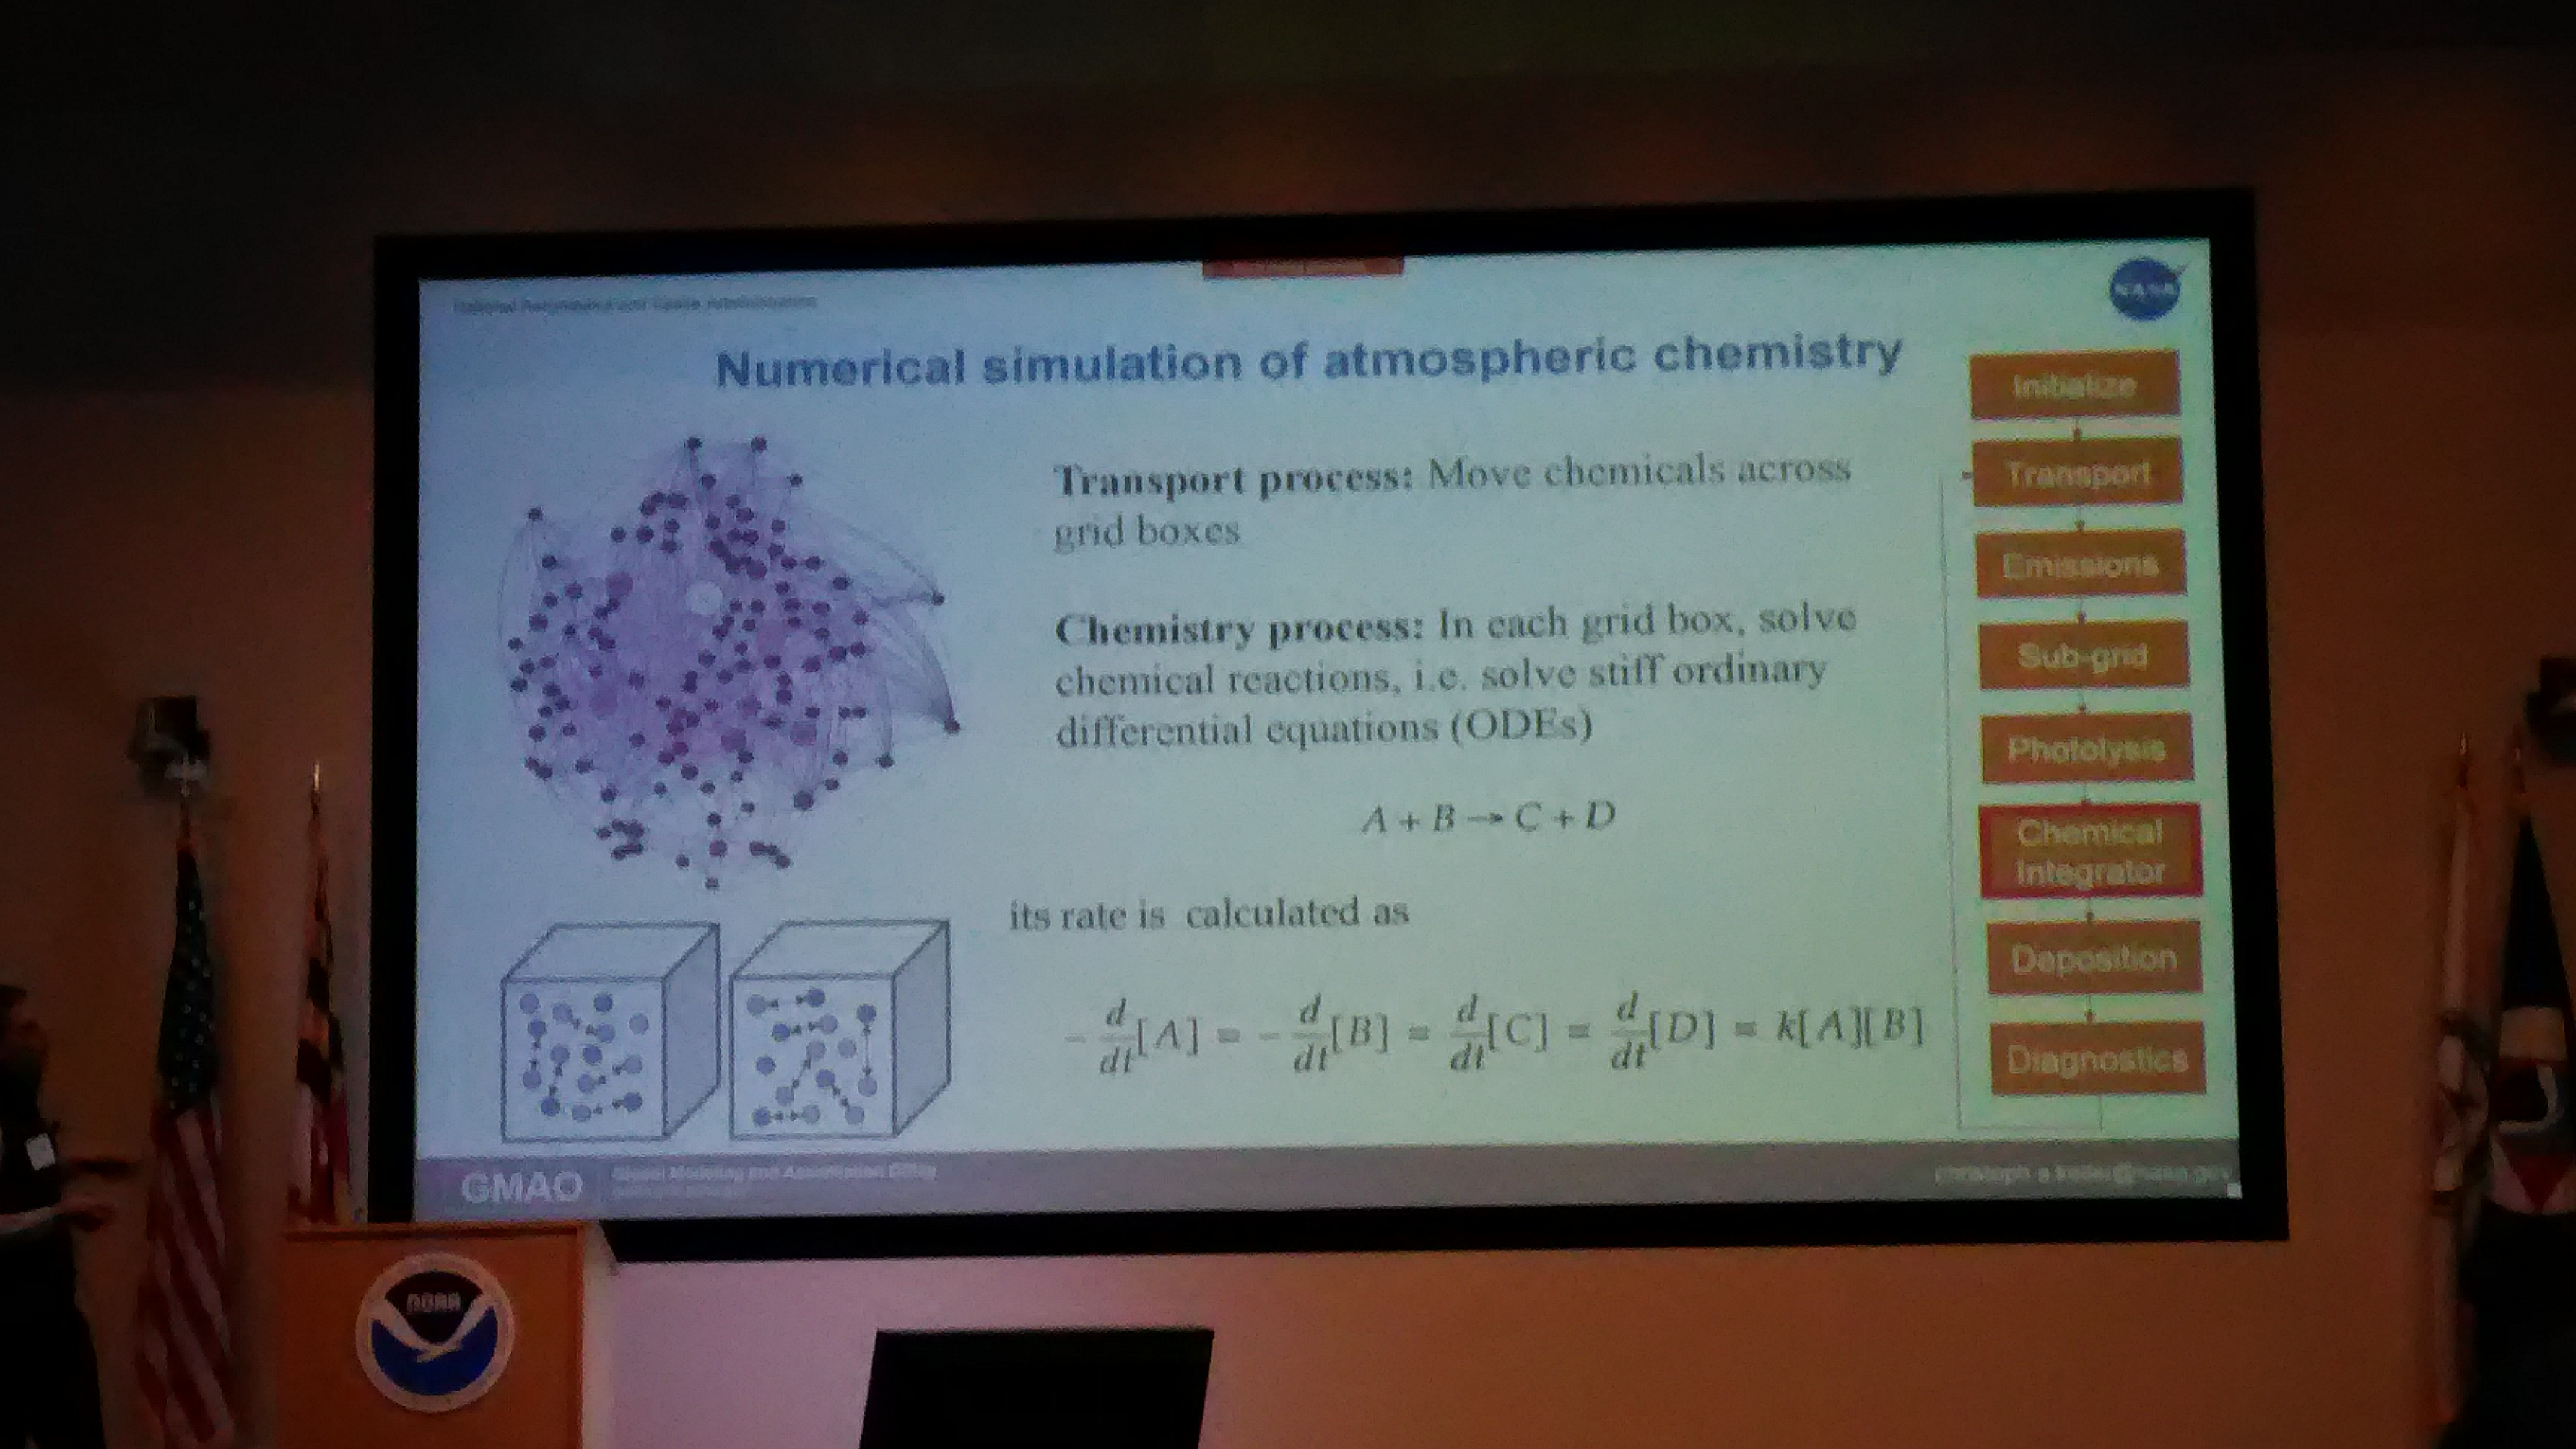
\includegraphics[width=.9\linewidth]{figs/P_20190425_085723.jpg}
\end{figure}
\end{frame}


\begin{frame}
\frametitle{Christoph Keller, NASA/GMAO \textit{(Atmospheric chemistry and air forecasting using machine learning)}}
\begin{figure}
	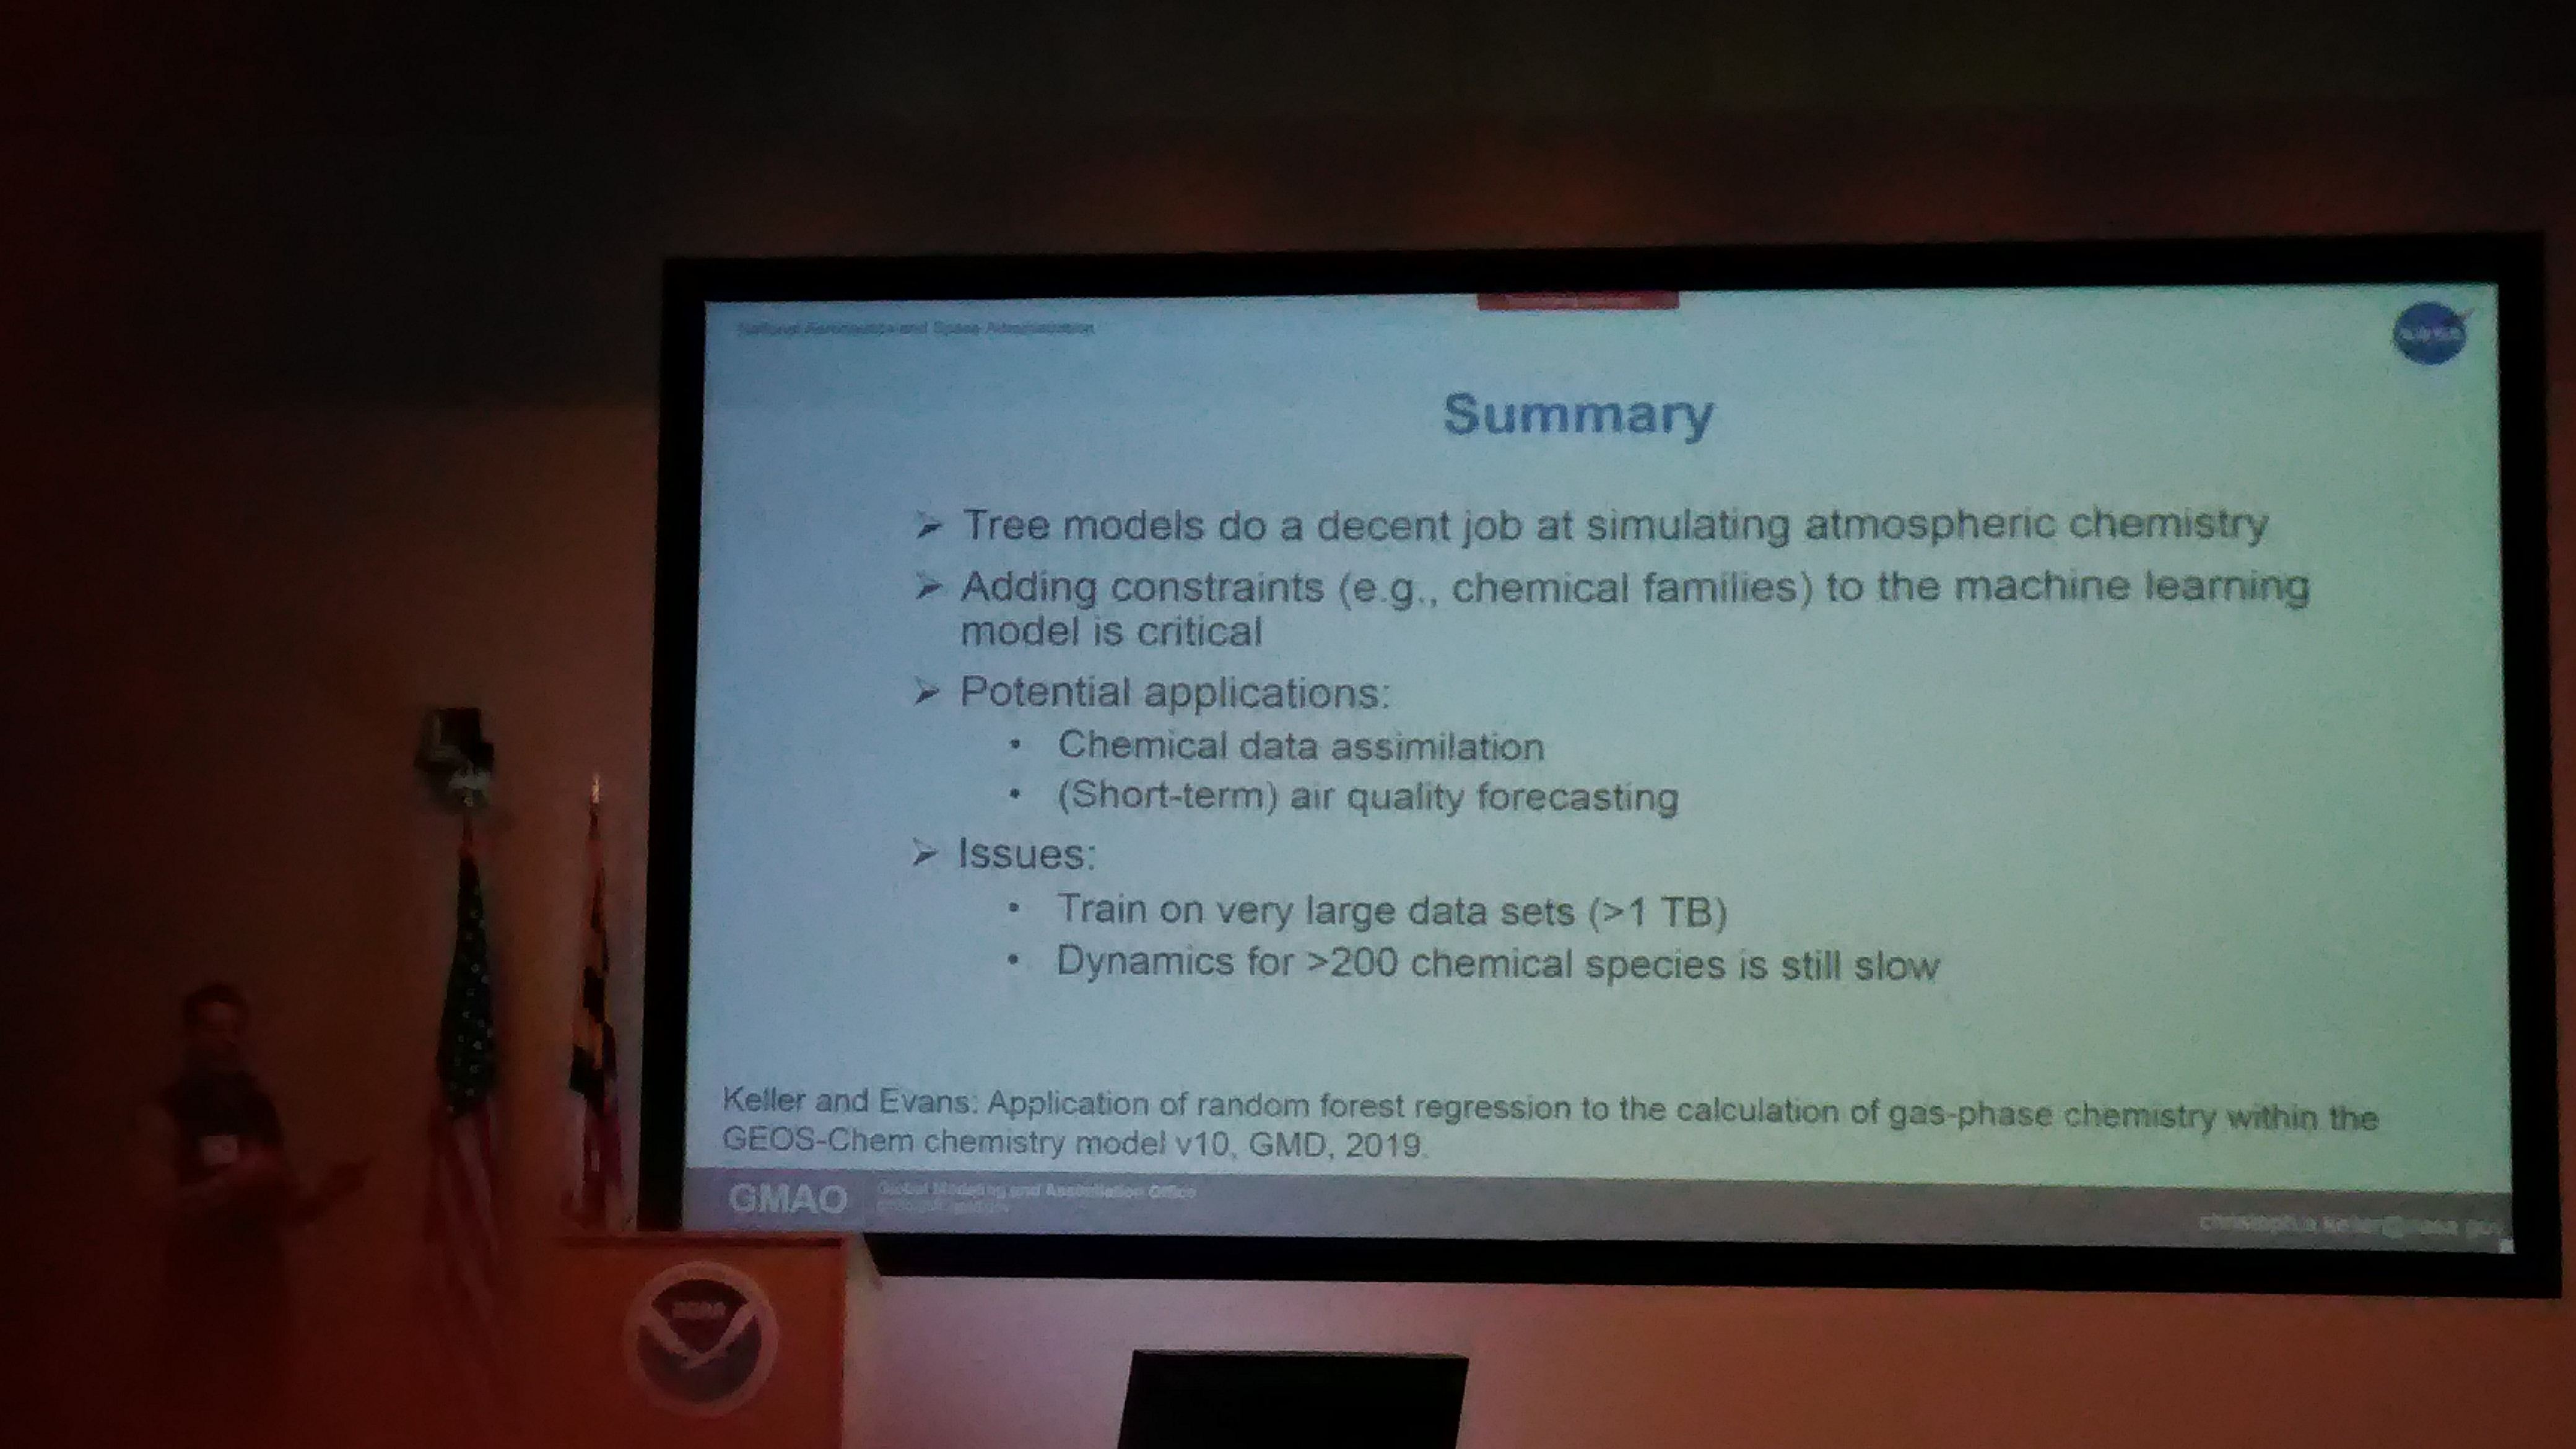
\includegraphics[width=.9\linewidth]{figs/P_20190425_090846.jpg}
\end{figure}
\end{frame}


\begin{frame}
\frametitle{Eric Kihn, NOAA/NESDIS \textit{(Analog Forecast Models for Space Weather Prediction)}}
\begin{figure}
	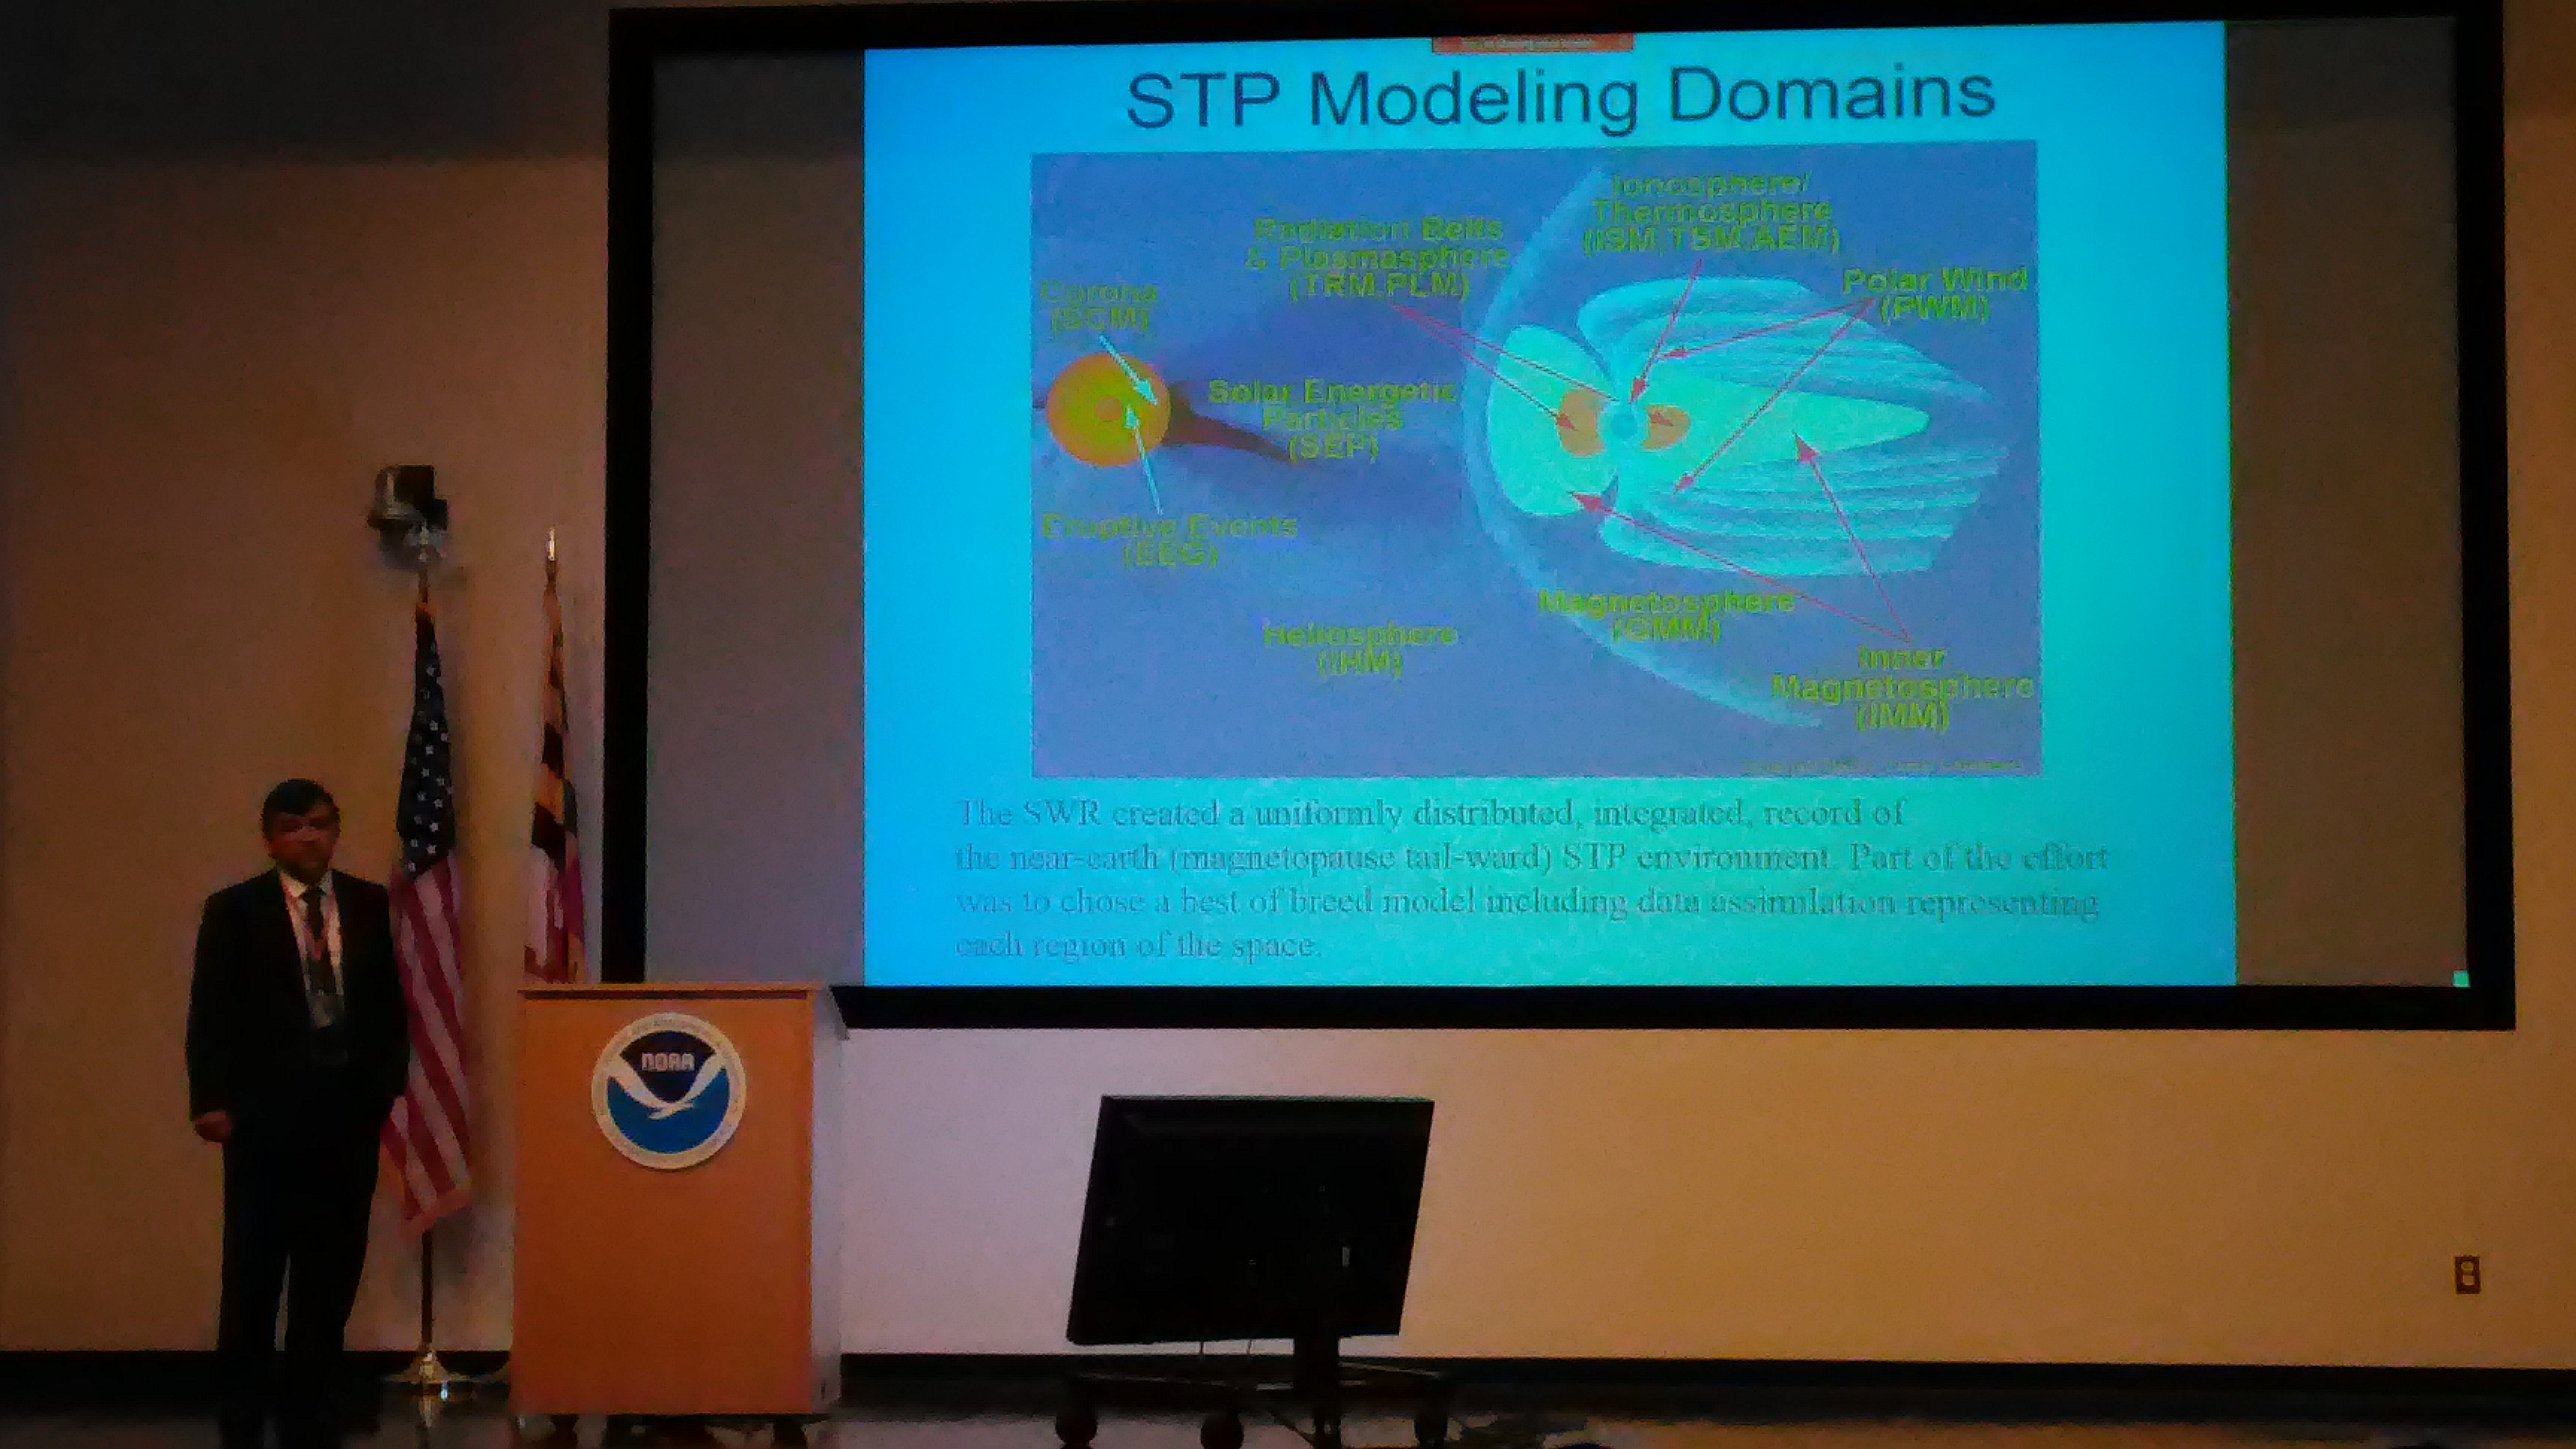
\includegraphics[width=.9\linewidth]{figs/P_20190425_093405.jpg}
\end{figure}
\end{frame}



%
%\begin{frame}
%\frametitle{Outline} % Table of contents slide, comment this block out to remove it
%\tableofcontents[currentsection] % Throughout your presentation, if you choose to use \section{} and \subsection{} commands, these will automatically be printed on this slide as an overview of your presentation
%\end{frame}
%
%\begin{frame}
%\frametitle{Fused Deep Learning for Hurricane Track Forecast} % Table of contents slide, comment this block out to remove it
%\textit{Joint work with Mo Yang, Claire Monteleoni and Guillaume Charpiat}\\
%\begin{figure}
%	\includegraphics[width=0.7\linewidth]{figs/hurricane-florence-2018-monday-radar.jpg}
%	\caption{Hurricane Florence, Monday radar.}
%\end{figure}
%\end{frame}


%\begin{frame}
%\frametitle{Hurricanes}
%
%\begin{figure}
%	\includegraphics[width=0.6\linewidth, height=0.6\textheight]{figs/Katrina.png}
%	\includegraphics[width=0.3\linewidth, height=0.4\textheight]{figs/saffir-simpson.png}
%\end{figure}
%\begin{itemize}
%\item Hurricane Katrina, 2005. (1 dot every 6 hours).\\
%\item \textbf{Tracks} and \textbf{Intensity} : Two main goals of the forecast
%\end{itemize}
%\end{frame}
%
%\subsection{Problem Setting}
%\begin{frame}
%\frametitle{Problem Setting}
%\begin{itemize}
%	\item Goal: estimating the 24h-forecast trajectory of all tropical storms.  \\
%\end{itemize}
%\begin{figure}
%	\includegraphics[width=0.8\linewidth]{figs/storm_shema.png}
%\end{figure}
%\end{frame}
%
%\subsection{Data Description}
%
%\begin{frame}
%\frametitle{Data sources}
%	\begin{figure}
%		\includegraphics[width=0.7\linewidth]{figs/all_storms.png}
%		\label{fig: storm_tracks}
%		\caption{Database: 3000 tropical/extra-tropical storm tracks since 1979. (NOAA database IBTrACS, every 6h)}
%	\end{figure}
%
%\end{frame}
%
%\begin{frame}
%\frametitle{Data sources}
%\begin{itemize}
%	\item \textbf{Reanalysis data:} 
%	\begin{itemize}
%		\item Global atmospheric grids : wind fields, pressure, temperature, humidity... 
%		\item Whole planet (resolution: 80km), 60 vertical levels, every 6h
%	\end{itemize}
%	\begin{figure}
%	\centering
%		\includegraphics[width=0.33\linewidth]{figs/reanalysis_grid.jpg}
%		\hfill
%		\includegraphics[width=0.46\linewidth]{figs/hurricane_schema.pdf}
%	\end{figure}
%\end{itemize}
%\end{frame}
%
%\subsection{Fused CNN}
%\begin{frame}
%\frametitle{Learn 24h-track forecast from conv. neural network}
%\begin{itemize}
%	\item  Three-stream fusion network \\
%\end{itemize}
%\begin{figure}
%	\includegraphics[width=1.0\linewidth]{figs/fusion_network.pdf}
%\end{figure}
%\end{frame}
%
%\begin{frame}
%\frametitle{Training a Fusion Network}
%\begin{itemize}
%	\item  Stage \Rmnum{1}: Train separate networks \\
%	\item  Stage \Rmnum{2}: Train the fusion network \\
%	\begin{itemize}
%		\item  Zoom in fusion layers:
%		\begin{figure}
%			\flushleft
%			\includegraphics[width=0.65\linewidth]{figs/fusion_details.pdf} \\
%		\end{figure}
%		\item Add connections between different streams in fusion layers
%		\item Re-train the whole network
%		%item two-phase optimization:
%		%	\begin{itemize}
%		%		\item first phase: optimize weights only in fusion layers
%		%		\item second phase: optimize weights in all layers
%		%	\end{itemize}
%	\end{itemize}
%\end{itemize}
%\end{frame}
%
%\subsection{Results}
%\begin{frame}
%\frametitle{Experiments}
%\framesubtitle{Selecting Fusion Network Configuration}
%\begin{figure}
%	\caption{24h-forecast results: distance between predicted and real location.}
%	\includegraphics[width=0.6\linewidth]{figs/MAE.PNG} \\
%\end{figure}
%
%\centering{
%\small{Btw, naive fusion's forecasting error =\textbf{142.63 km}...\\}
%\small{worse than best single stream alone! }
%}
%\end{frame}
%
%\begin{frame}
%\frametitle{Experiments}
%\framesubtitle{Comparison with the Existing Forecasting Models}
%Qualitative: 
%
%\begin{figure}
%	\includegraphics[width=1.0\linewidth]{figs/one_stom_result.png}\\
%	\caption{The forecast errors of the three models (left: the OCFL, middle: the BCD5, right: our fusion network) on the Hurricane Ian in 2016}
%\end{figure}
%\end{frame}
%
%
%
%%------------------------------------------------
%\section{Create Your Hackathon / Challenge} % Sections can be created in order to organize your presentation into discrete blocks, all sections and subsections are automatically printed in the table of contents as an overview of the talk
%%------------------------------------------------
%\subsection{Climate Informatics Hackathon}
%
%\begin{frame}
%\frametitle{Outline} % Table of contents slide, comment this block out to remove it
%\tableofcontents[currentsection] % Throughout your presentation, if you choose to use \section{} and \subsection{} commands, these will automatically be printed on this slide as an overview of your presentation
%\end{frame}
%
%
%\begin{frame}
%
%\frametitle{Climate Informatics Hackathon}
%
%\begin{itemize}
%	\item CI workshop
%	\begin{figure}
%	\includegraphics[width=0.65\linewidth]{figs/CI_2018.jpg} \\
%\end{figure}
%	\item One-day hackathon (CS + climatologists)
%	\item Machine learning problem on climate
%	\item This year : hurricane \textbf{intensity} forecasting
%	\item Using the Ramp Studio framework
%
%\end{itemize}
%
%\end{frame}
%
%\begin{frame}
%\frametitle{Hurricanes (remember...)}
%
%\begin{figure}
%	\includegraphics[width=0.6\linewidth, height=0.6\textheight]{figs/Katrina.png}
%	\includegraphics[width=0.3\linewidth, height=0.4\textheight]{figs/saffir-simpson.png}
%\end{figure}
%\begin{itemize}
%\item Hurricane Katrina, 2005. (1 dot every 6 hours).\\
%\item \textbf{Tracks} and \textbf{Intensity} : Two main goals of the forecast
%\end{itemize}
%\end{frame}
%
%
%\subsection{Ramp Studio}
%
%\begin{frame}
%\frametitle{RAMP?}
%\begin{itemize}
%\item What? Collaborative platform for data science challenges 
%\item Where? Paris Saclay
%\item Why?
%	\begin{itemize}
%		\item Kaggle-like contests...
%		\item but submit (python) code! Models are trained on a back-end.
%		\item And then, open phase: all participants have access to all code
%	\end{itemize}
%	
%\item For who?
%	\begin{itemize}
%		\item Anybody can make a ramp (hackathon/challenge)
%		\item Code is open (Git)
%		\item Good for learning (and teaching)
%		\item Good for research too..
%	\end{itemize}
%\end{itemize}
%
%\href{https://youtu.be/vQoH68hb85Q}{\beamergotobutton{Link to video}}
%\href{https://www.ramp.studio}{\beamergotobutton{Link to RAMP}}
%\href{https://github.com/ramp-kits/storm_forecast}{\beamergotobutton{Link to Git}}
%
%\end{frame}





\begin{frame}

\frametitle{Thank you!}
Any questions?
%\begin{figure}
%	\includegraphics[width=0.65\linewidth]{figs/pipeline.png} \\
%\end{figure}

\end{frame}




\end{document}
